\documentclass[journal]{new-aiaa}
% \documentclass[conf]{new-aiaa} %for conference papers
\usepackage[utf8]{inputenc}

\usepackage{graphicx}
\usepackage{amsmath}
\usepackage[version=4]{mhchem}
\usepackage{siunitx}
\usepackage{longtable,tabularx}
\setlength\LTleft{0pt}

% \usepackage{amsmath}          % for formula writing (i.e. 'split', etc)
\usepackage{rotate}           %rotate/mirror images
\usepackage{cancel}           %draw lines through math to show "goes to zero"
\usepackage{xfrac}            %allows slated and side fractions
\usepackage{subcaption}       %allows captioning individual subfigures
\usepackage[mode=buildnew]{standalone}% requires -shell-escape
  % compile with `pdflatex -shell-escape main` or `xelatex  -shell-escape main`

\usepackage{float} %Force figures to exact location in doc (use '[H]' option)

\usepackage{tikz}             %for creating vector graphics diagrams
\usetikzlibrary{backgrounds}  %put backgrounds behind tikz figures
\usetikzlibrary{calc}         %perform calculations within $$
\usetikzlibrary{positioning}  %position tikz elements using "right of, etc"
\usetikzlibrary{angles}       %label angles between lines with arcs
\usetikzlibrary{quotes}       %Put angle label in quotes
\usetikzlibrary{patterns}     %Patterns to fill shapes with




\title{Review of Analysis and Modeling Techniques for Incompressible, Turbulent Bluff-Body Wakes}

\author{Logan D. Halstrom\footnote{Graduate Student, Mechanical And Aerospace Engineering Department, One Shields Avenue} and Federico Zabaleta\footnote{Graduate Student, Civil and Environmental Engineering Department, One Shields Avenue}}
\affil{University of California, Davis, California, 95616}



%%%%%%%%%%%%%%%%%%%%%%%%%%%%%%%%%%%%%%%%%%%%%%%%%%%%%%%%%%%%%%%%%%%%%%%%
\begin{document}

\maketitle

%%%%%%%%%%%%%%%%%%%%%%%%%%%%%%%%%%%%%%%%%%%%%%%%%%%%%%%%%%%%%%%%%%%%%%%%
\begin{abstract} %%%%%%%%%%%%%%%%%%%%%%%%%%%%%%%%%%%%%%%%%%%%%%%%%%%%%%%
%%%%%%%%%%%%%%%%%%%%%%%%%%%%%%%%%%%%%%%%%%%%%%%%%%%%%%%%%%%%%%%%%%%%%%%%

\textcolor{red}{abstract here}
\textcolor{red}{\emph{LH\&FZ}}

\end{abstract}



%%%%%%%%%%%%%%%%%%%%%%%%%%%%%%%%%%%%%%%%%%%%%%%%%%%%%%%%%%%%%%%%%%%%%%%%
\section*{Nomenclature} %%%%%%%%%%%%%%%%%%%%%%%%%%%%%%%%%%%%%%%%%%%%%%%%
%%%%%%%%%%%%%%%%%%%%%%%%%%%%%%%%%%%%%%%%%%%%%%%%%%%%%%%%%%%%%%%%%%%%%%%%

\textcolor{red}{\emph{LH\&FZ}}

{\renewcommand\arraystretch{1.0}
\noindent\begin{longtable*}{@{}l @{\quad=\quad} l@{}}
$\rho$ & density, $kg/m^3$\\
\multicolumn{2}{@{}l}{Subscripts}\\
$()_{\infty}$ & freestream quantity\\
\multicolumn{2}{@{}l}{Acronyms}\\
CFD & Computational Fluid Dynamics\\
\end{longtable*}}



%%%%%%%%%%%%%%%%%%%%%%%%%%%%%%%%%%%%%%%%%%%%%%%%%%%%%%%%%%%%%%%%%%%%%%%%
\section{Introduction} \label{sec:intro}
%%%%%%%%%%%%%%%%%%%%%%%%%%%%%%%%%%%%%%%%%%%%%%%%%%%%%%%%%%%%%%%%%%%%%%%%




\lettrine{B}{odies} When a body moves in a fluid, it experience different forces, such as lift and drag. Drag can occur due to a difference in velocity in the surface of the body and the mean flow, in which case we call it friction drag. This friction is associated with the development of boundary layers and is it scales with the Reynolds number. If the drag is due to a difference in pressure trough the surface of the body, then we call it pressure drag or viscous induced drag. This drag is usually associated with separation of the flow and the formation of a wake downstream the body. In real flows, drag is composed by the combination of both. The effect of frictional drag is usually more relevant for attached flows while the pressure drag prevails in separated flows.

We can analyze the effect of friction and pressure drag by analyzing the flow around a flat plate. If the flat plate is oriented in the direction of the flow, then the friction drag will be important while the pressure drag will be almost negligible. On the other side, if the orient the flat plate perpendicular to the flow, then the difference of pressure between both sides of the plate will be much more important than the effect of the friction, and so the pressure drag will be dominant.

When the drag of a body is dominated by viscous drag, we define the body as a streamlined body. Flat plates (oriented in the direction of the flow) or  airfoils with a small angle of attack are examples of those. When the flow is dominated by pressure drag, we define the body as a bluff or blunt body. Examples or these are squares, cylinders, spheres or airfoil at large angle of attack. Whether a body is considered bluff or streamlined is only a function of its shape and its orientation with respect to the flow.

\begin{center}
\textcolor{red}{INSERT FIGURE}
\end{center}



\section{Flow around a bluff body and transition}

\begin{figure}[H]
\begin{center}
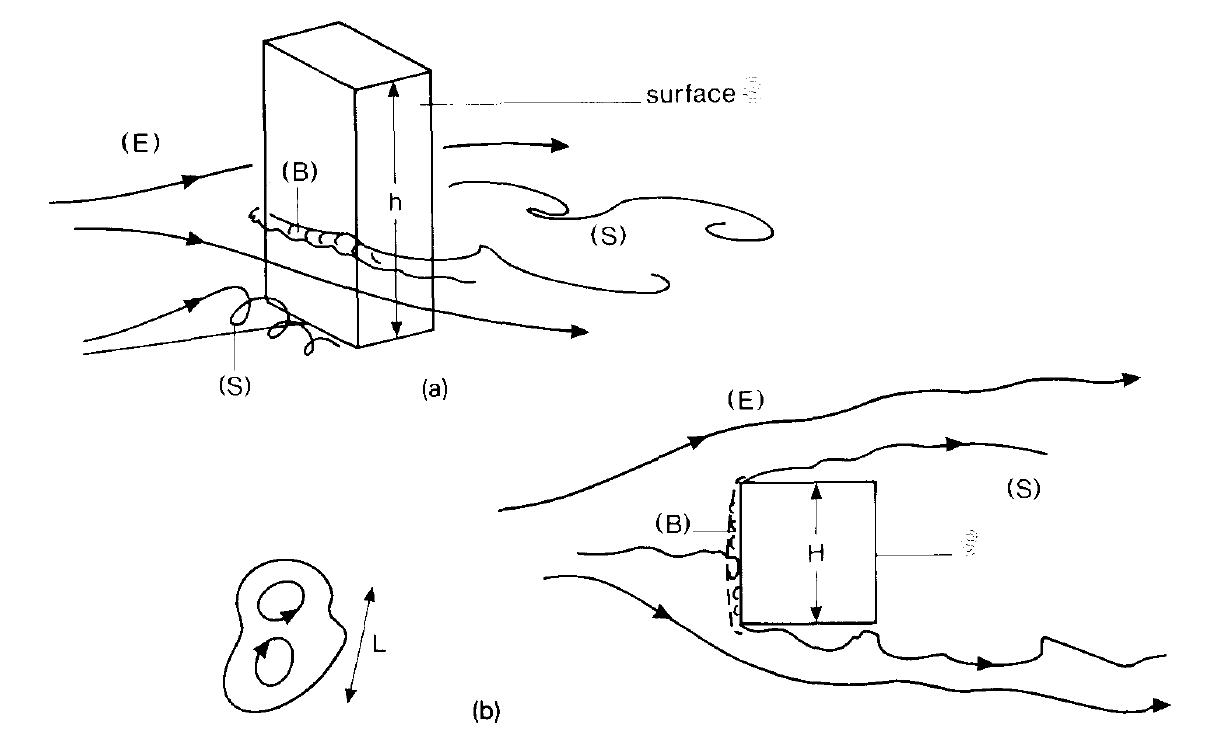
\includegraphics[width=0.7\textwidth]{Images/federico/Figure01}
\caption{ Regions of disturbed flow. Extracted from \cite{hunt1990} }
\label{fig:RegionsFlow}
\end{center}
\end{figure}

\subsection{Steady laminar wake}

\subsection{Periodic Laminar Regime}


\begin{figure}[H]
\begin{center}
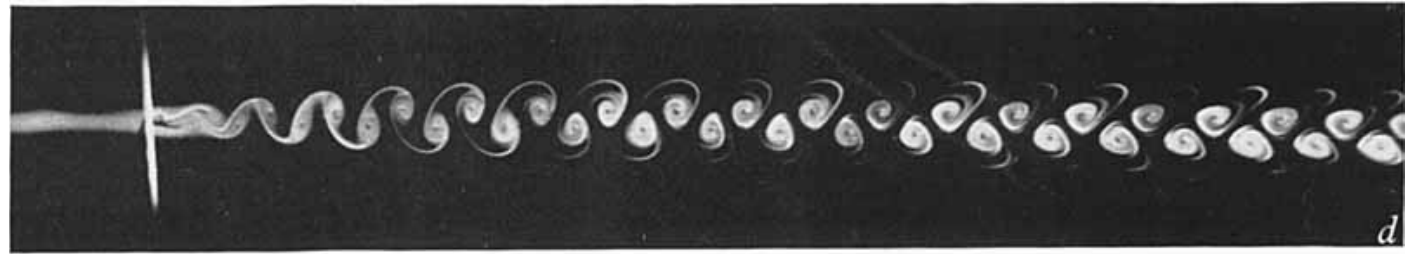
\includegraphics[width=1\textwidth]{Images/federico/Figure02}
\caption{Kárman-Bénard eddy street at \textbf{\textit{Re = 100}}. Extracted from \cite{Zdravkovich1968} }
\label{fig:Laminar}
\end{center}
\end{figure}

\subsection{Transition in wake state}

\begin{figure}[H]
\begin{center}
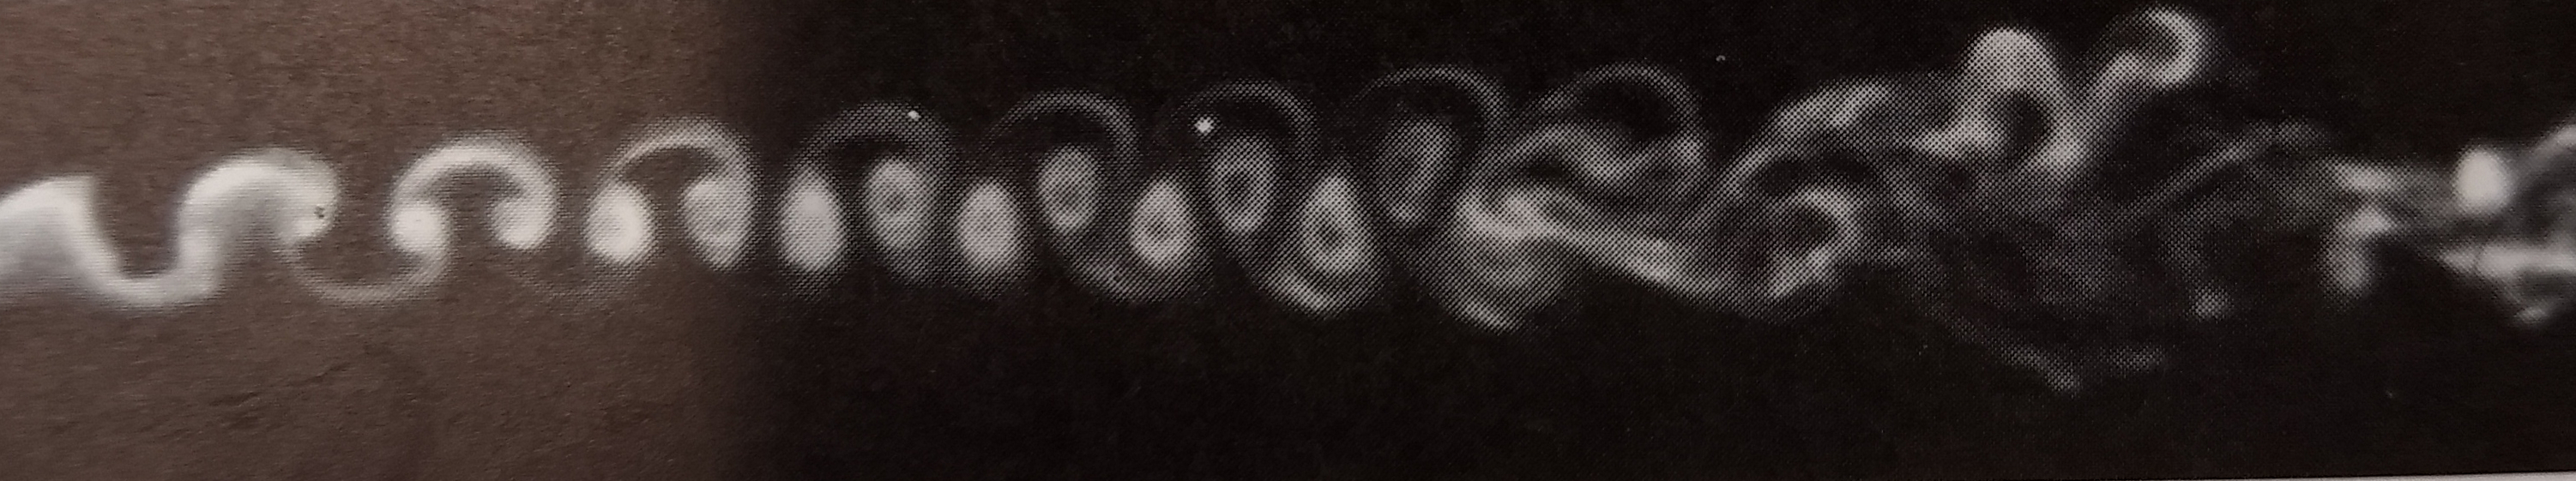
\includegraphics[width=1\textwidth]{Images/federico/Figure03}
\caption{Transition in wake at \textbf{\textit{Re = 190}}. Extracted from \cite{Zdravkovich1968} }
\label{fig:TrW1}
\end{center}
\end{figure}

\begin{figure}[H]
\begin{center}
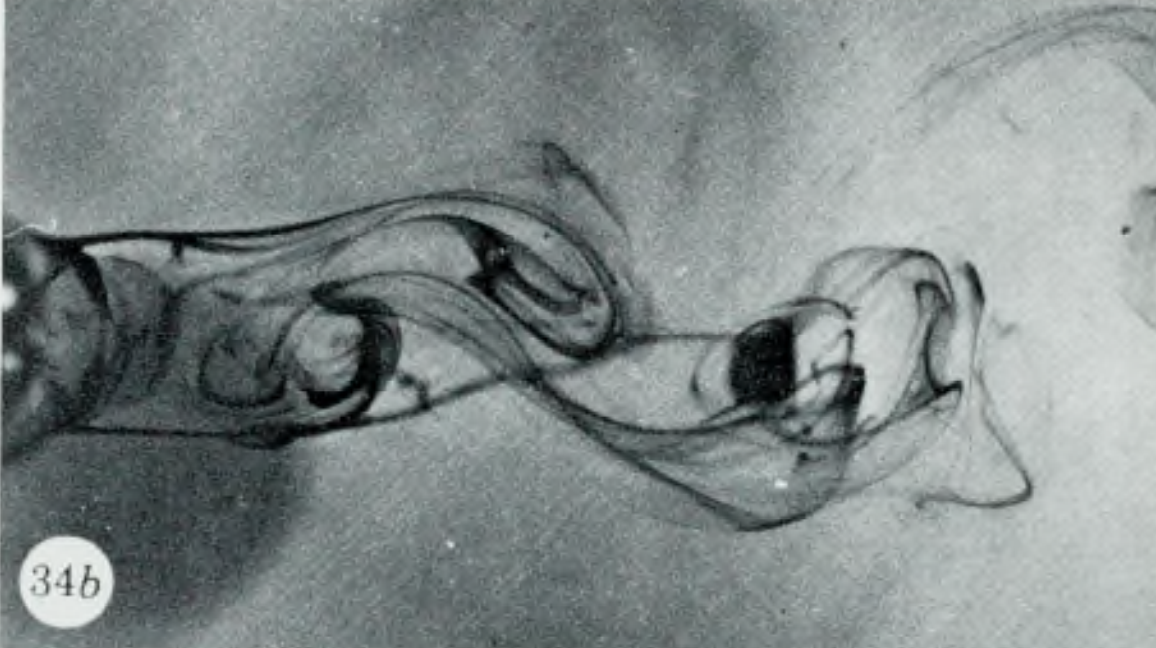
\includegraphics[width=0.5\textwidth]{Images/federico/Figure04}
\caption{Transition in wake at \textbf{\textit{Re = 344}}. Extracted from \cite{Gerrard1978} }
\label{fig:TrW2}
\end{center}
\end{figure}

\subsection{Transition in shear layers state}

\begin{figure}[H]
\begin{center}
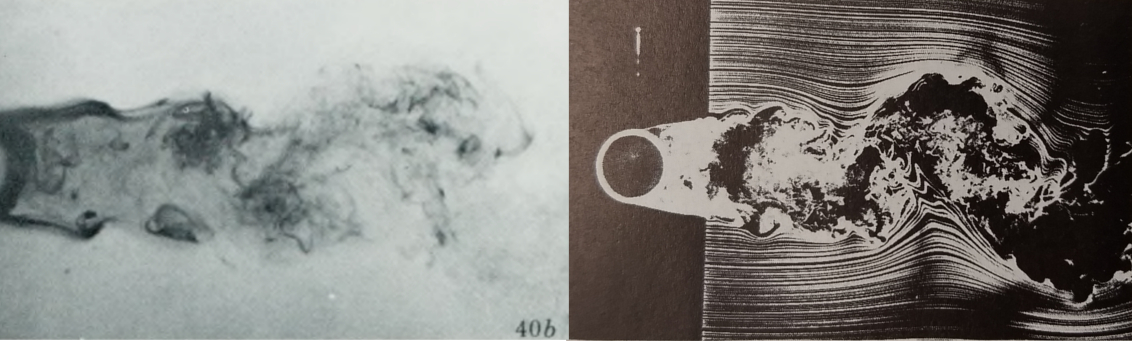
\includegraphics[width=1\textwidth]{Images/federico/Figure05}
\caption{Transition in free shear layer. Left: \textbf{\textit{Re = 1083}}. Extracted from \cite{Gerrard1978}. Right: \textbf{\textit{Re = 8000}}. Extracted from \cite{Zdravkovich1997}}
\label{fig:TrSL}
\end{center}
\end{figure}

\subsection{Transition in boundary layer}

\subsection{Fully turbulent state}


\section{Free stream turbulence and non-uniform free stream}

\begin{itemize}
    \item Driving Physical Phenomena \textcolor{red}{\emph{FZ}}

    \begin{itemize}
        \item differences from potential flow
        \item blunt/bluff body definition, differences from streamlined body flow
        \item massively separated flow
        \item base pressure
        \item wake
    \end{itemize}
    \item Real World Applications \textcolor{red}{\emph{LH}}
    \begin{itemize}
        \item parachute
        \item reentry capsule
        \item vehicles
        \item buildings
        \item show similarity between cylinder/sphere wake and more complex bluff body
    \end{itemize}
\end{itemize}






\emph{Big whorls have little whorls, which feed on their velocity, and little whorls have lesser whorls, and so on to viscosity (in the molecular sense).}
Richardson (1922) \cite{richardson1922weather}




%%%%%%%%%%%%%%%%%%%%%%%%%%%%%%%%%%%%%%%%%%%%%%%%%%%%%%%%%%%%

%%% BLUFF BODY FLAME HOLDER
%%\vspace{-2em}
% \begin{figure}[htb]
\begin{figure}[H]
\begin{center}
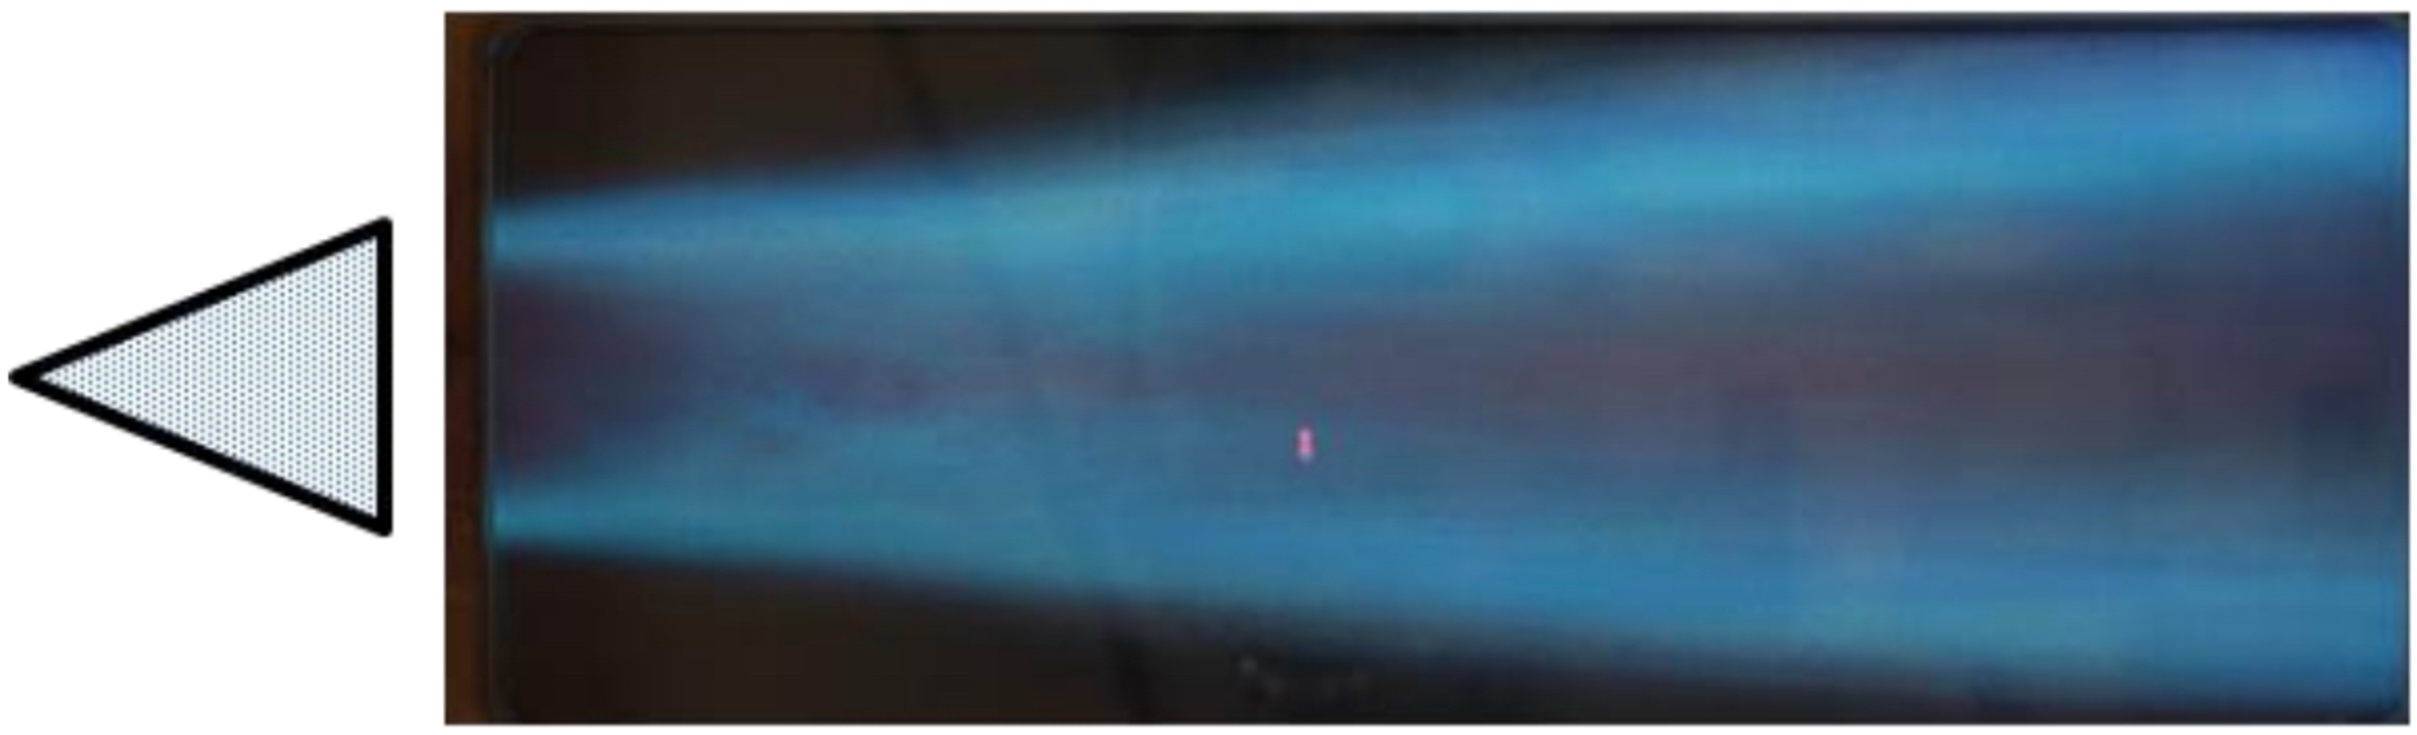
\includegraphics[width=0.5\textwidth]{Images/logan/tanaka2013bluff_FlameHolder.pdf}
\caption{ Bluff-body flame holder \cite{tanaka2013bluff} }
\label{fig:flameholder}
\end{center}
\end{figure}
%%\vspace{-2em}


Bluff body stabilized flame is widely used in various industrial systems in which the flow speed is much higher than the flame speed. Without a continuous ignition source the flame would be blown out. Hence the gutter/bluff body is usually placed with its axis perpendicular to the flow direction. The gutter traps the hot gas downstream of the recirculation zone. The trapped hot gas acts as a continuous ignition source to hold and stabilize the flame. The gutter is usually called as a flame holder or a flame stabilizer \cite{li2011large}.





%%% ORION WAKE
%%\vspace{-2em}
% \begin{figure}[htb]
\begin{figure}[H]
\begin{center}
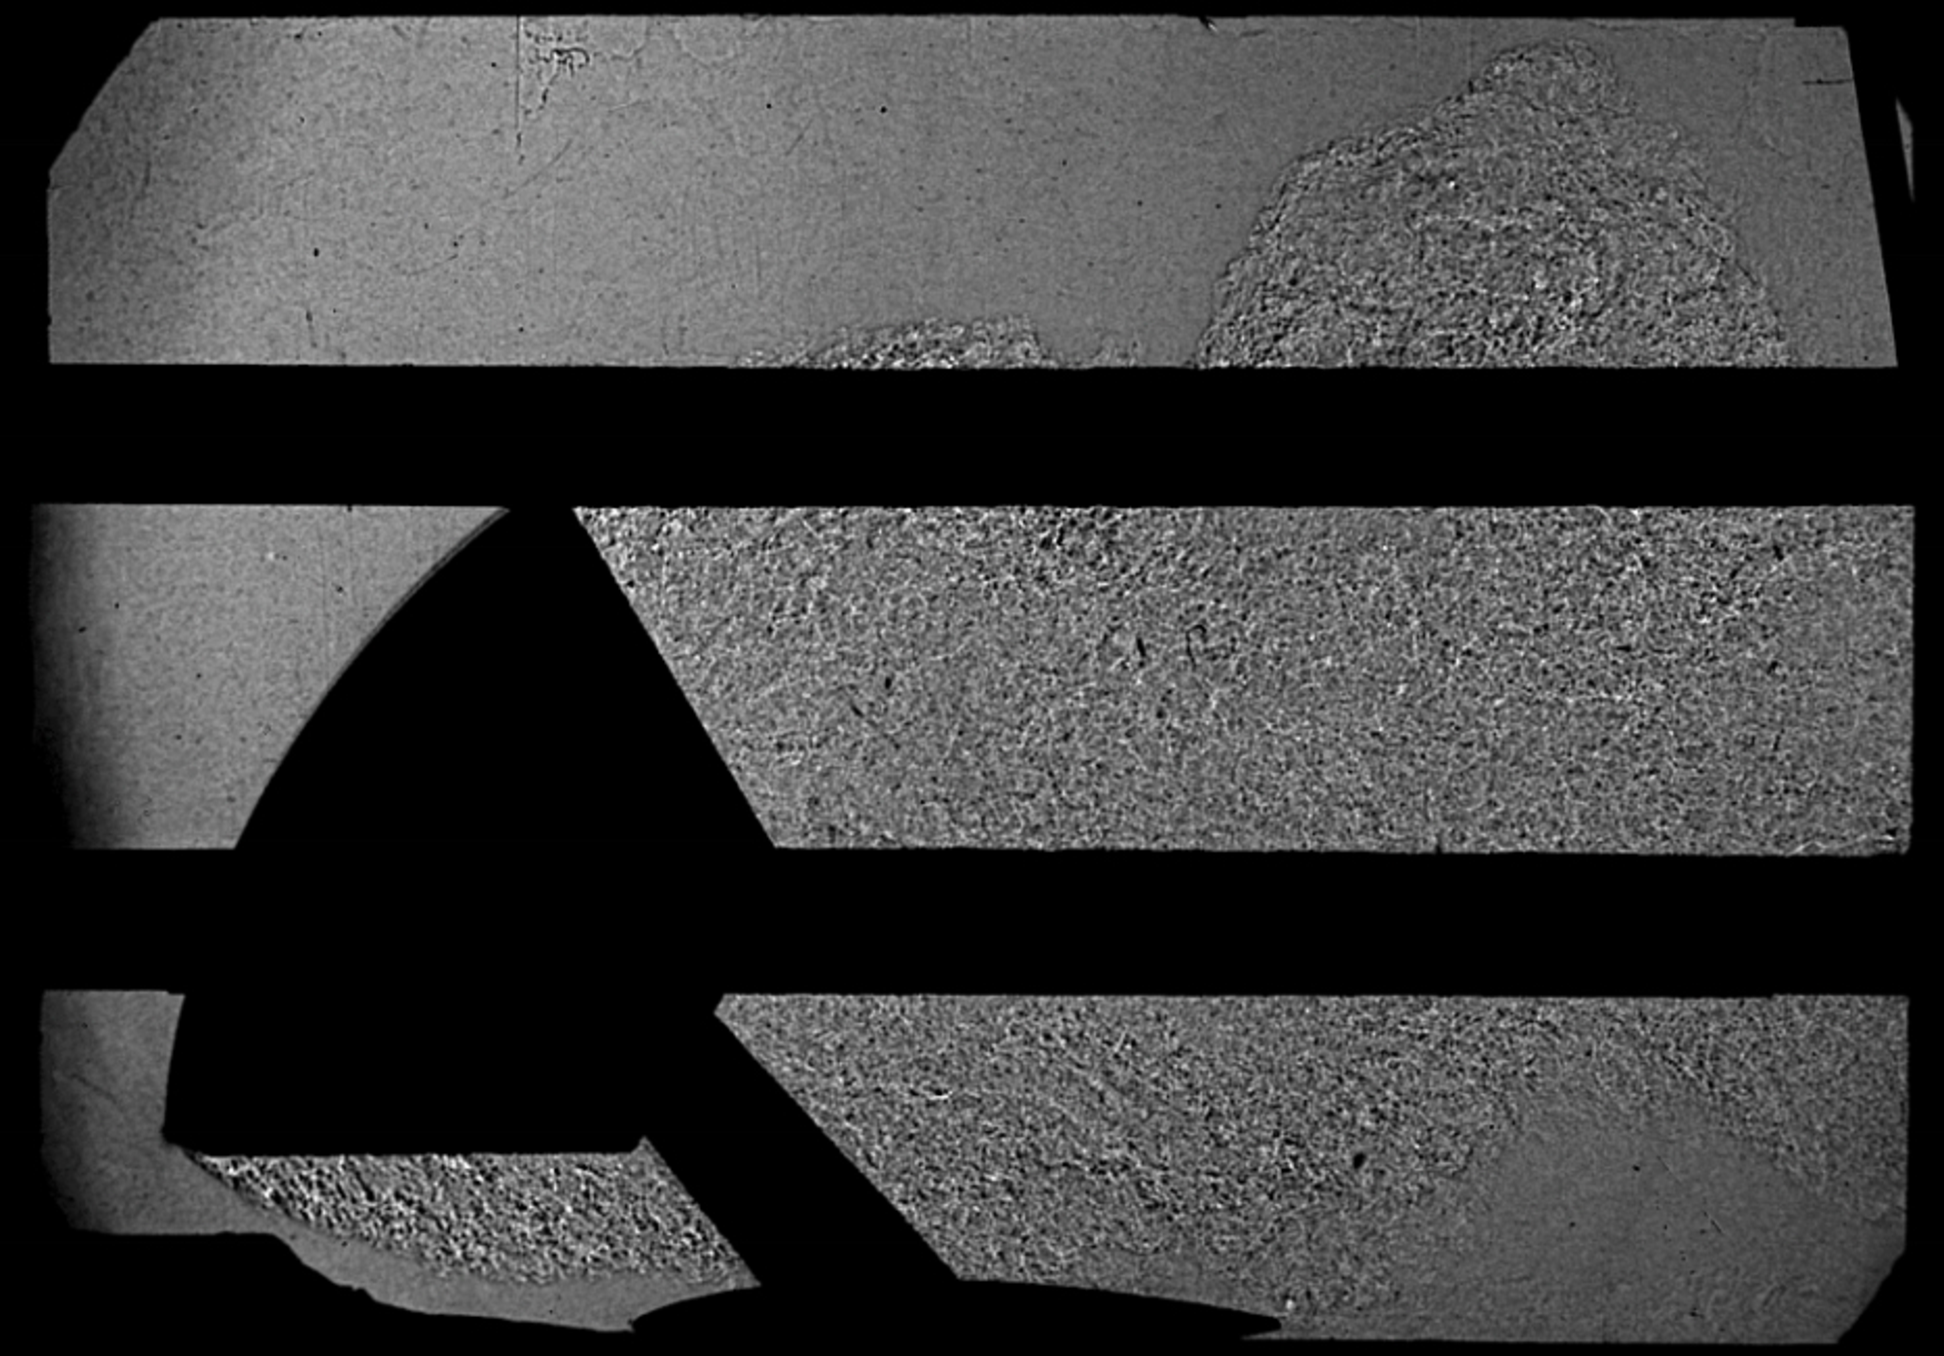
\includegraphics[width=0.5\textwidth]{Images/logan/ross2013comprehensive_CapsuleWakeShadowgraph.pdf}
\caption{ Shadowgraph wake of orion capsule model M=0.3 \cite{ross2013comprehensive} }
\label{fig:orionwakeshadowgraph}
\end{center}
\end{figure}
%%\vspace{-2em}

Single frame of high-speed shadowgraph
video; M 0.3, AoA = 29.25 deg, ReD = 5.3x106.




%%%%%%%%%%%%%%%%%%%%%%%%%%%%%%%%%%%%%%%%%%%%%%%%%%%%%%%%%%%%%%%%%%%%%%%%
\section{Experimental Methods And Results} \label{sec:experimentalmethods}
%%%%%%%%%%%%%%%%%%%%%%%%%%%%%%%%%%%%%%%%%%%%%%%%%%%%%%%%%%%%%%%%%%%%%%%%

\textcolor{red}{\emph{FZ}}

\begin{itemize}
    \item Historical Study
    \item Experimental techniques
    \begin{itemize}
        \item ballistic range?
    \end{itemize}
    \item Applications
    \begin{itemize}
        \item Simple cases: cylinder/sphere
        \begin{itemize}
            \item Drag vs Re?
            \item Wake velocity profiles?
            \item Wake structure?
        \end{itemize}
        \item Sharp vs bluff: sphere vs cube
        \item Complex cases: capsule/building
    \end{itemize}
\end{itemize}








%%%%%%%%%%%%%%%%%%%%%%%%%%%%%%%%%%%%%%%%%%%%%%%%%%%%%%%%%%%%%%%%%%%%%%%%
\section{Computational Methods and Results} \label{sec:computationalmethods}
%%%%%%%%%%%%%%%%%%%%%%%%%%%%%%%%%%%%%%%%%%%%%%%%%%%%%%%%%%%%%%%%%%%%%%%%

\textcolor{red}{\emph{LH}}

\begin{itemize}
    \item Historical Study
    \item Computational techniques
    \item Applications
    \begin{itemize}
        \item Simple cases: cylinder/sphere
        \item Sharp vs bluff: sphere vs cube
        \item Complex cases: capsule/building
    \end{itemize}
\end{itemize}

%%%%%%%%%%%%%%%%%%%%%%%%%%%%%%%%%%%%%%%%%%%%%%%%%%%%%%%%%%%%%%%%%%%%%%%%
\subsection{Turbulence Modeling Aspects} \label{subsec:turbulencemodeling}

\textcolor{red}{\emph{LH}}

\begin{itemize}
    \item \underline{Brief} turbulence model description
    \begin{itemize}
        \item RANS vs URANS
        \item DNS
        \item LES (uses DNS) and DES (=Hybrid RANS/LES)
    \end{itemize}
    \item Compare turbulence model performance for sphere/cylinder
    \begin{itemize}
        \item DES > URANS > RANS
        \item DES = functional LES
        \item SAS vs DES?
        \item DNS: limited Re
    \end{itemize}
    \item Shortcomings of each model (and how to address them)
    \begin{itemize}
        \item URANS
        \item DES: only good at sharp separation
        \begin{itemize}
            \item ``An order of accuracy has not even been proposed for a simulation using both modes within DES'' -Spalart about hybrid method
            \item grid induced separation (maybe not an issue for bluff bodies)
            \item DES can default to RANS if grid adaptation misses a shear layer
    \end{itemize}
    \end{itemize}
    \item Advanced geometries
    \begin{itemize}
        \item f-15
        \item car
        \item building
        \item capsule
        \item chute, landing gear, helicopter, wind turbine
    \end{itemize}
\end{itemize}


LIST ALL FIGURES HEAR, REORDER AND DESCRIBE LATER


%%% SAS CYLINDER
%%\vspace{-2em}
% \begin{figure}[htb]
\begin{figure}[H]
\begin{center}
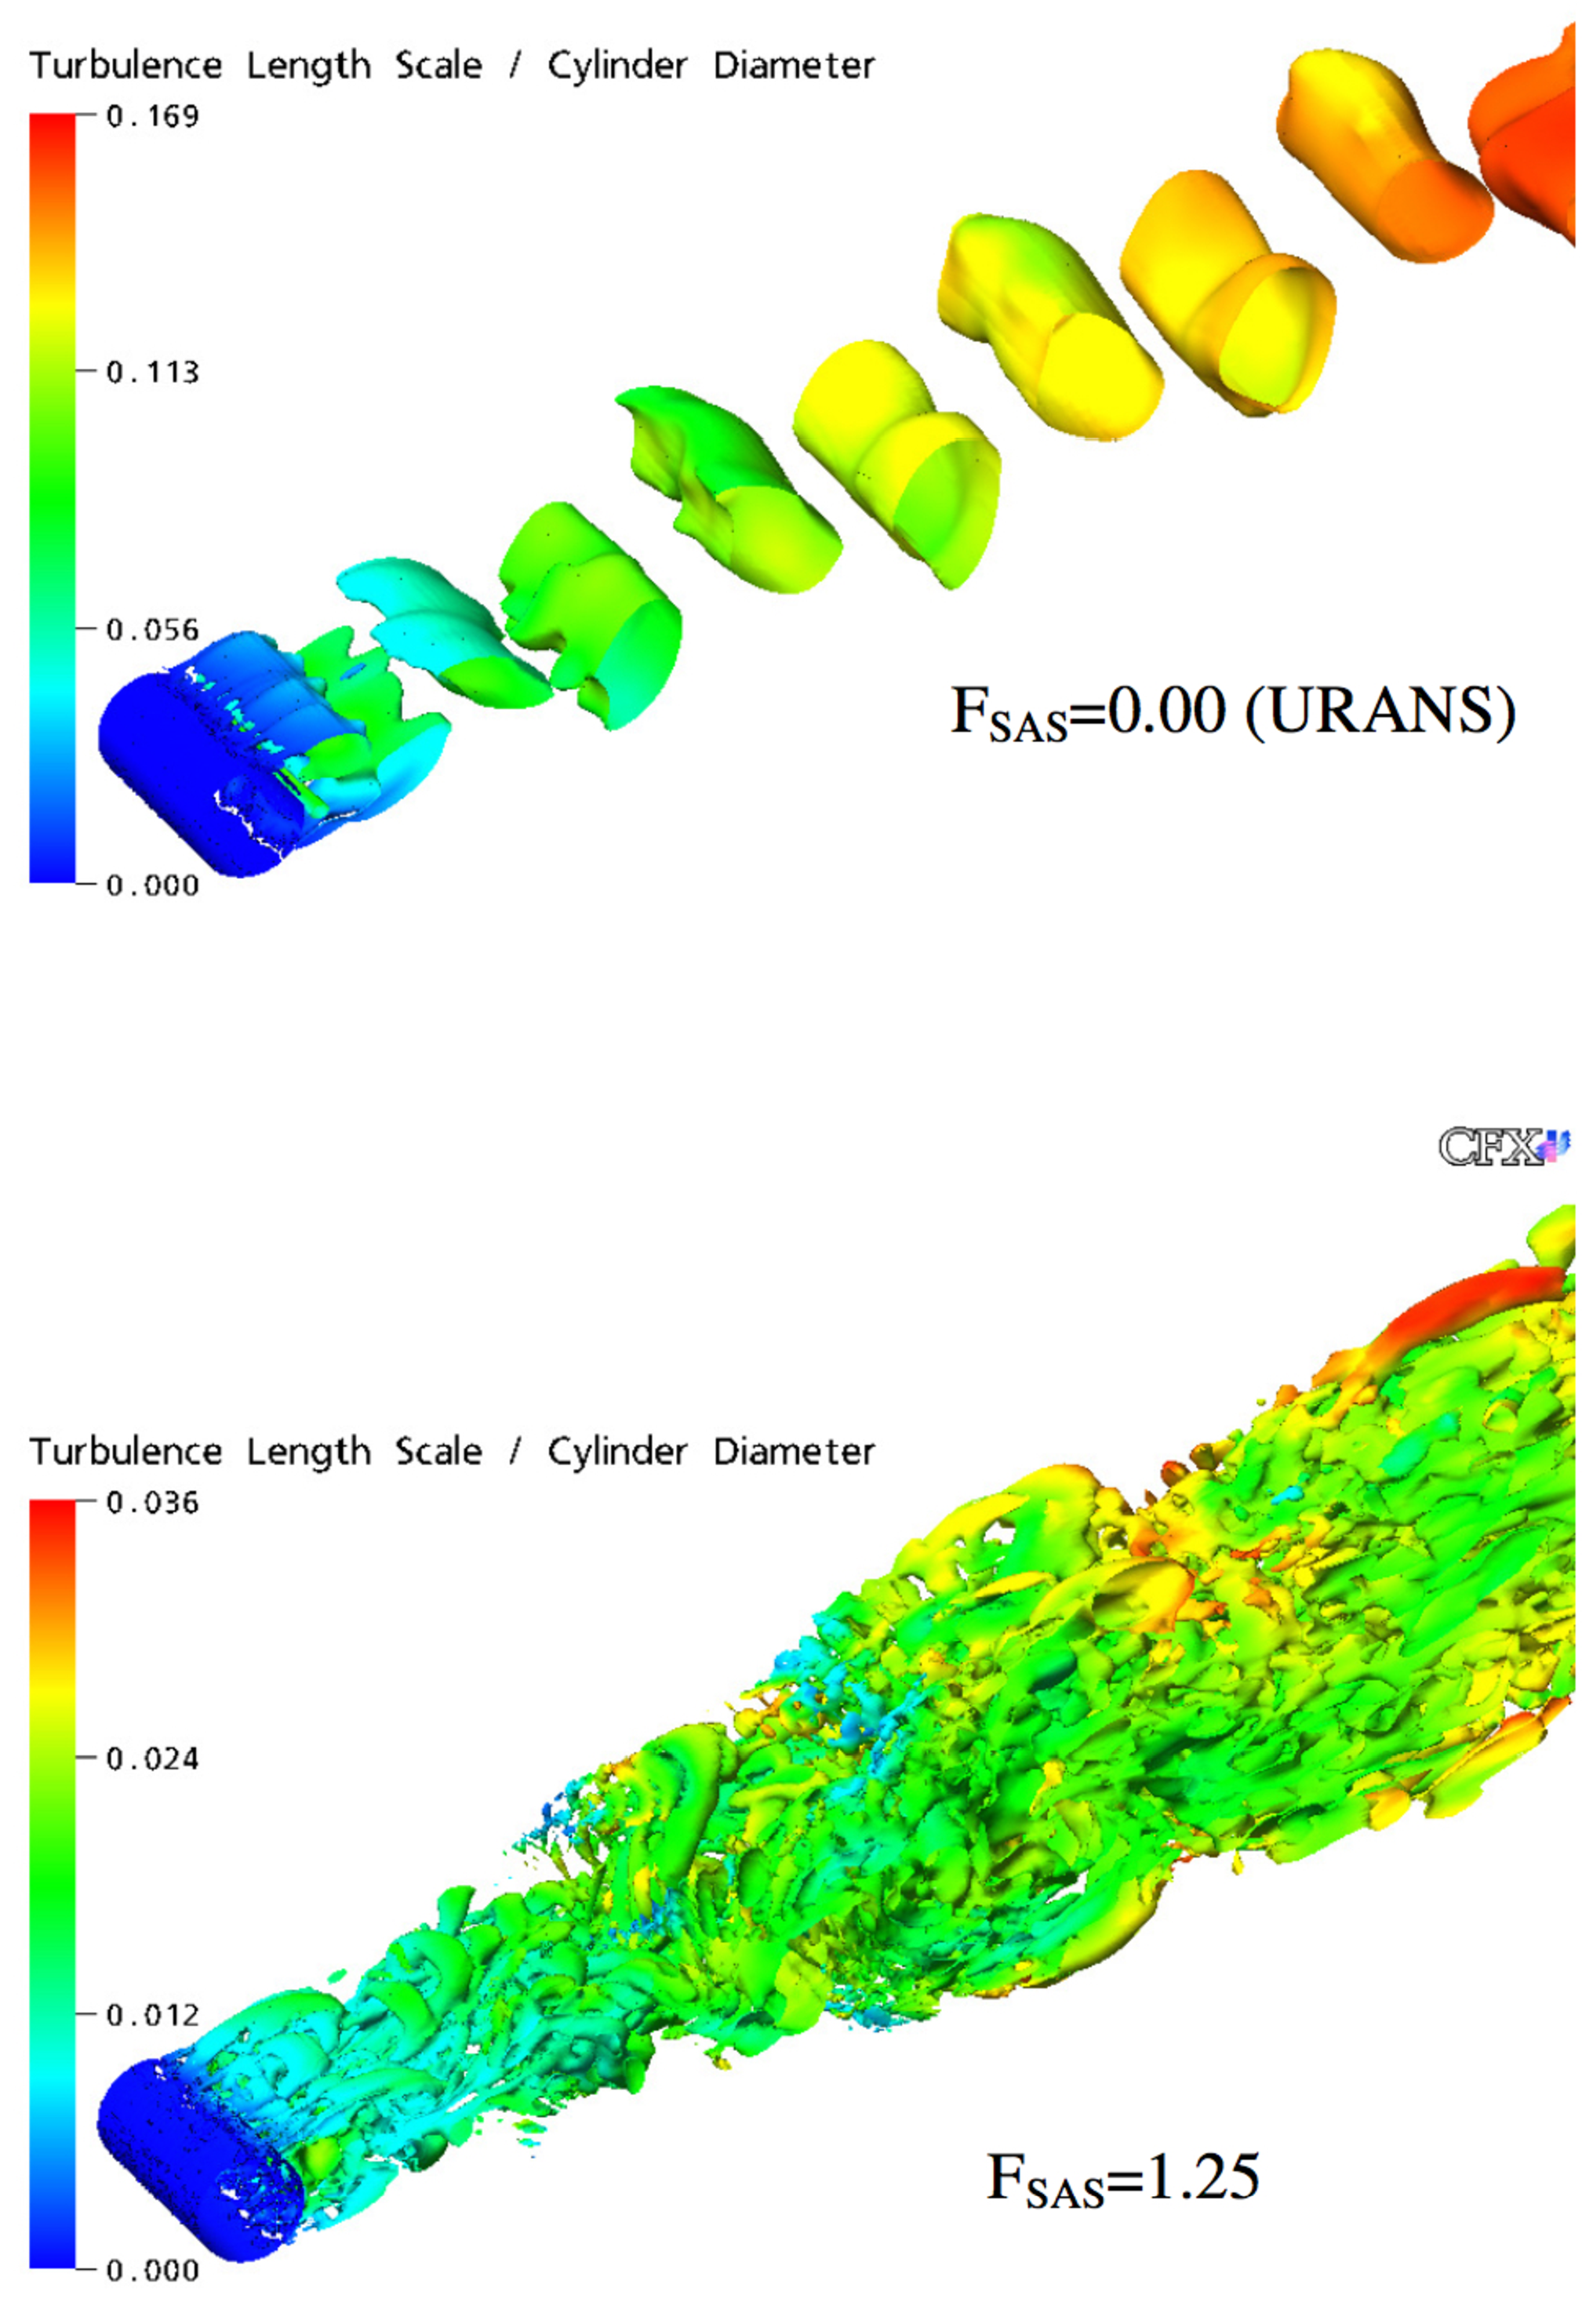
\includegraphics[width=0.5\textwidth]{Images/logan/menter2005scaleadaptive_cylinderwake2.pdf}
\caption{ SAS vs URANS cylinder \cite{menter2005scaleadaptive} }
\label{fig:sasvsuranscylinder}
\end{center}
\end{figure}
%%\vspace{-2em}

Figure 5: Resolved structures for cylinder in crossflow using different constants FSAS Re=3.6e6




%%% LES VS RANS CYLINDER
%%\vspace{-2em}
% \begin{figure}[htb]
\begin{figure}[H]
\begin{center}
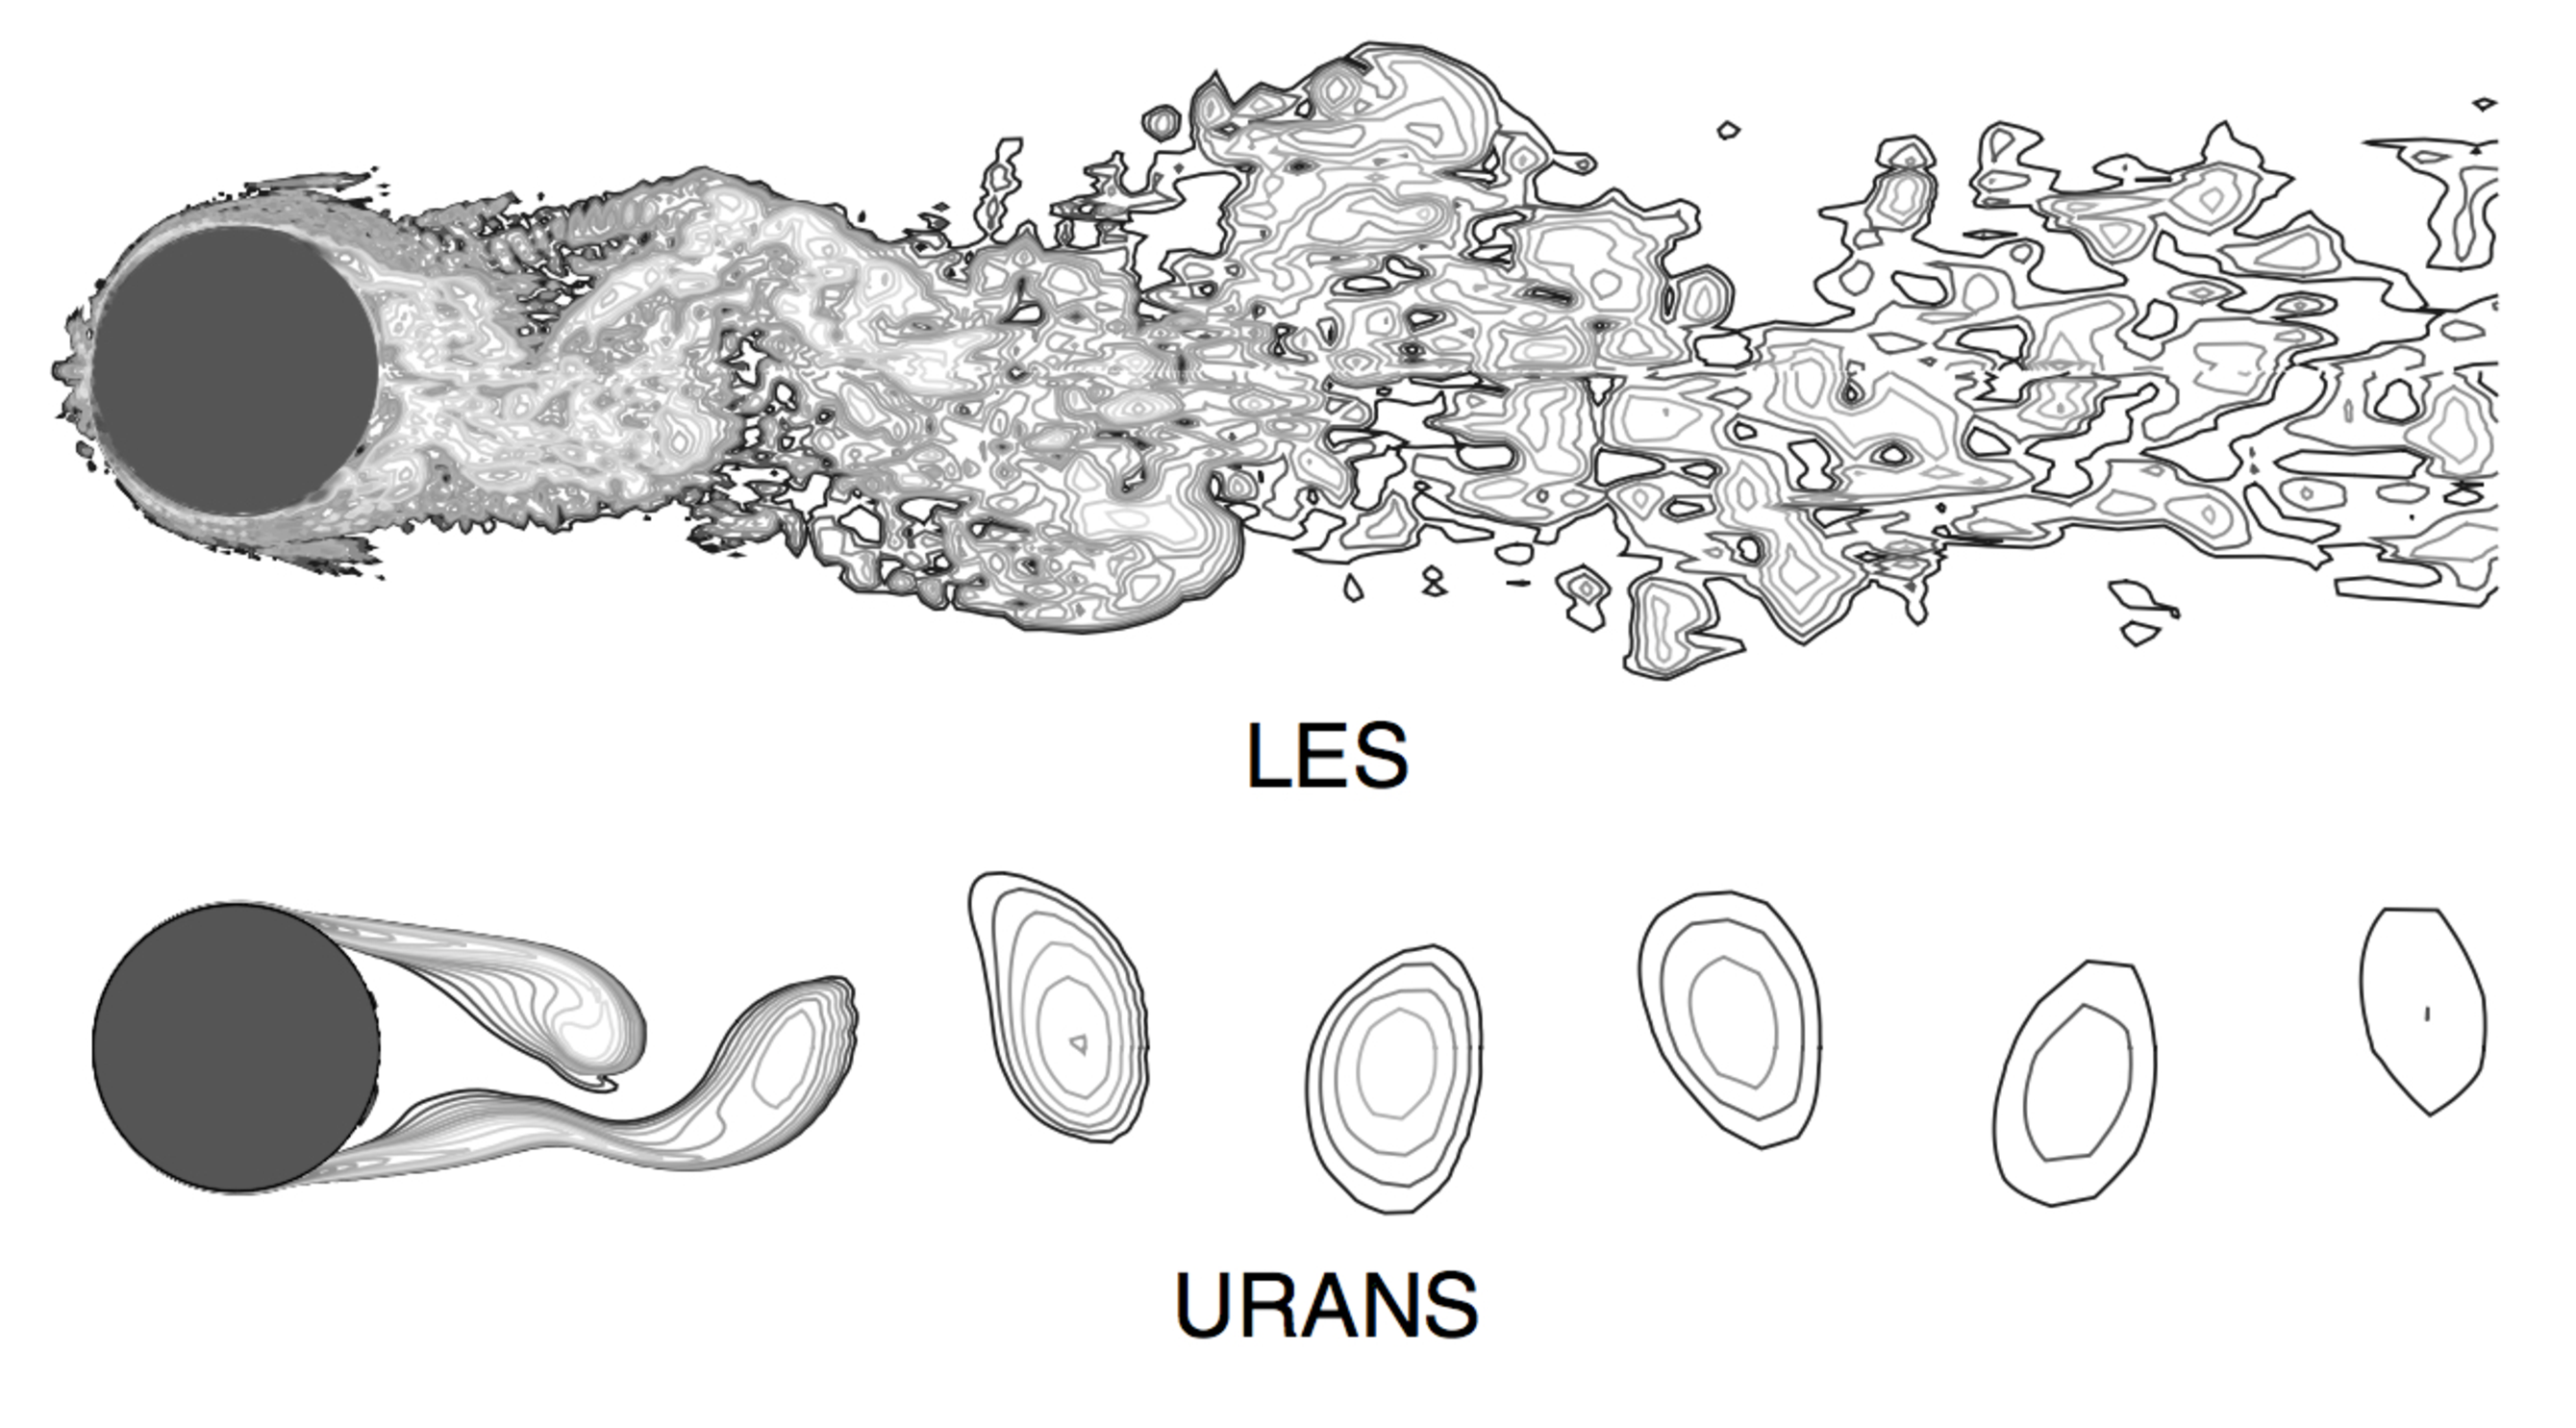
\includegraphics[width=0.5\textwidth]{Images/logan/catalano_2003numerical_UnsteadyURANSvsLES.pdf}
\caption{ cylinder les vs urans instantaneous \cite{catalano2003numerical} }
\label{fig:lesvsuranscylinderinstant}
\end{center}
\end{figure}
%%\vspace{-2em}

Instantaneous vorticity magnitude at a given spanwise cut for flow over a circular cylinder at ReD 1⁄4 1   106. 25 contour levels from xD=U1 1⁄4 1 to xD=U1 1⁄4 575 (exponential distribution) are plotted.


%%% LES VS RANS CYLINDER
%%\vspace{-2em}
% \begin{figure}[htb]
\begin{figure}[H]
\begin{center}
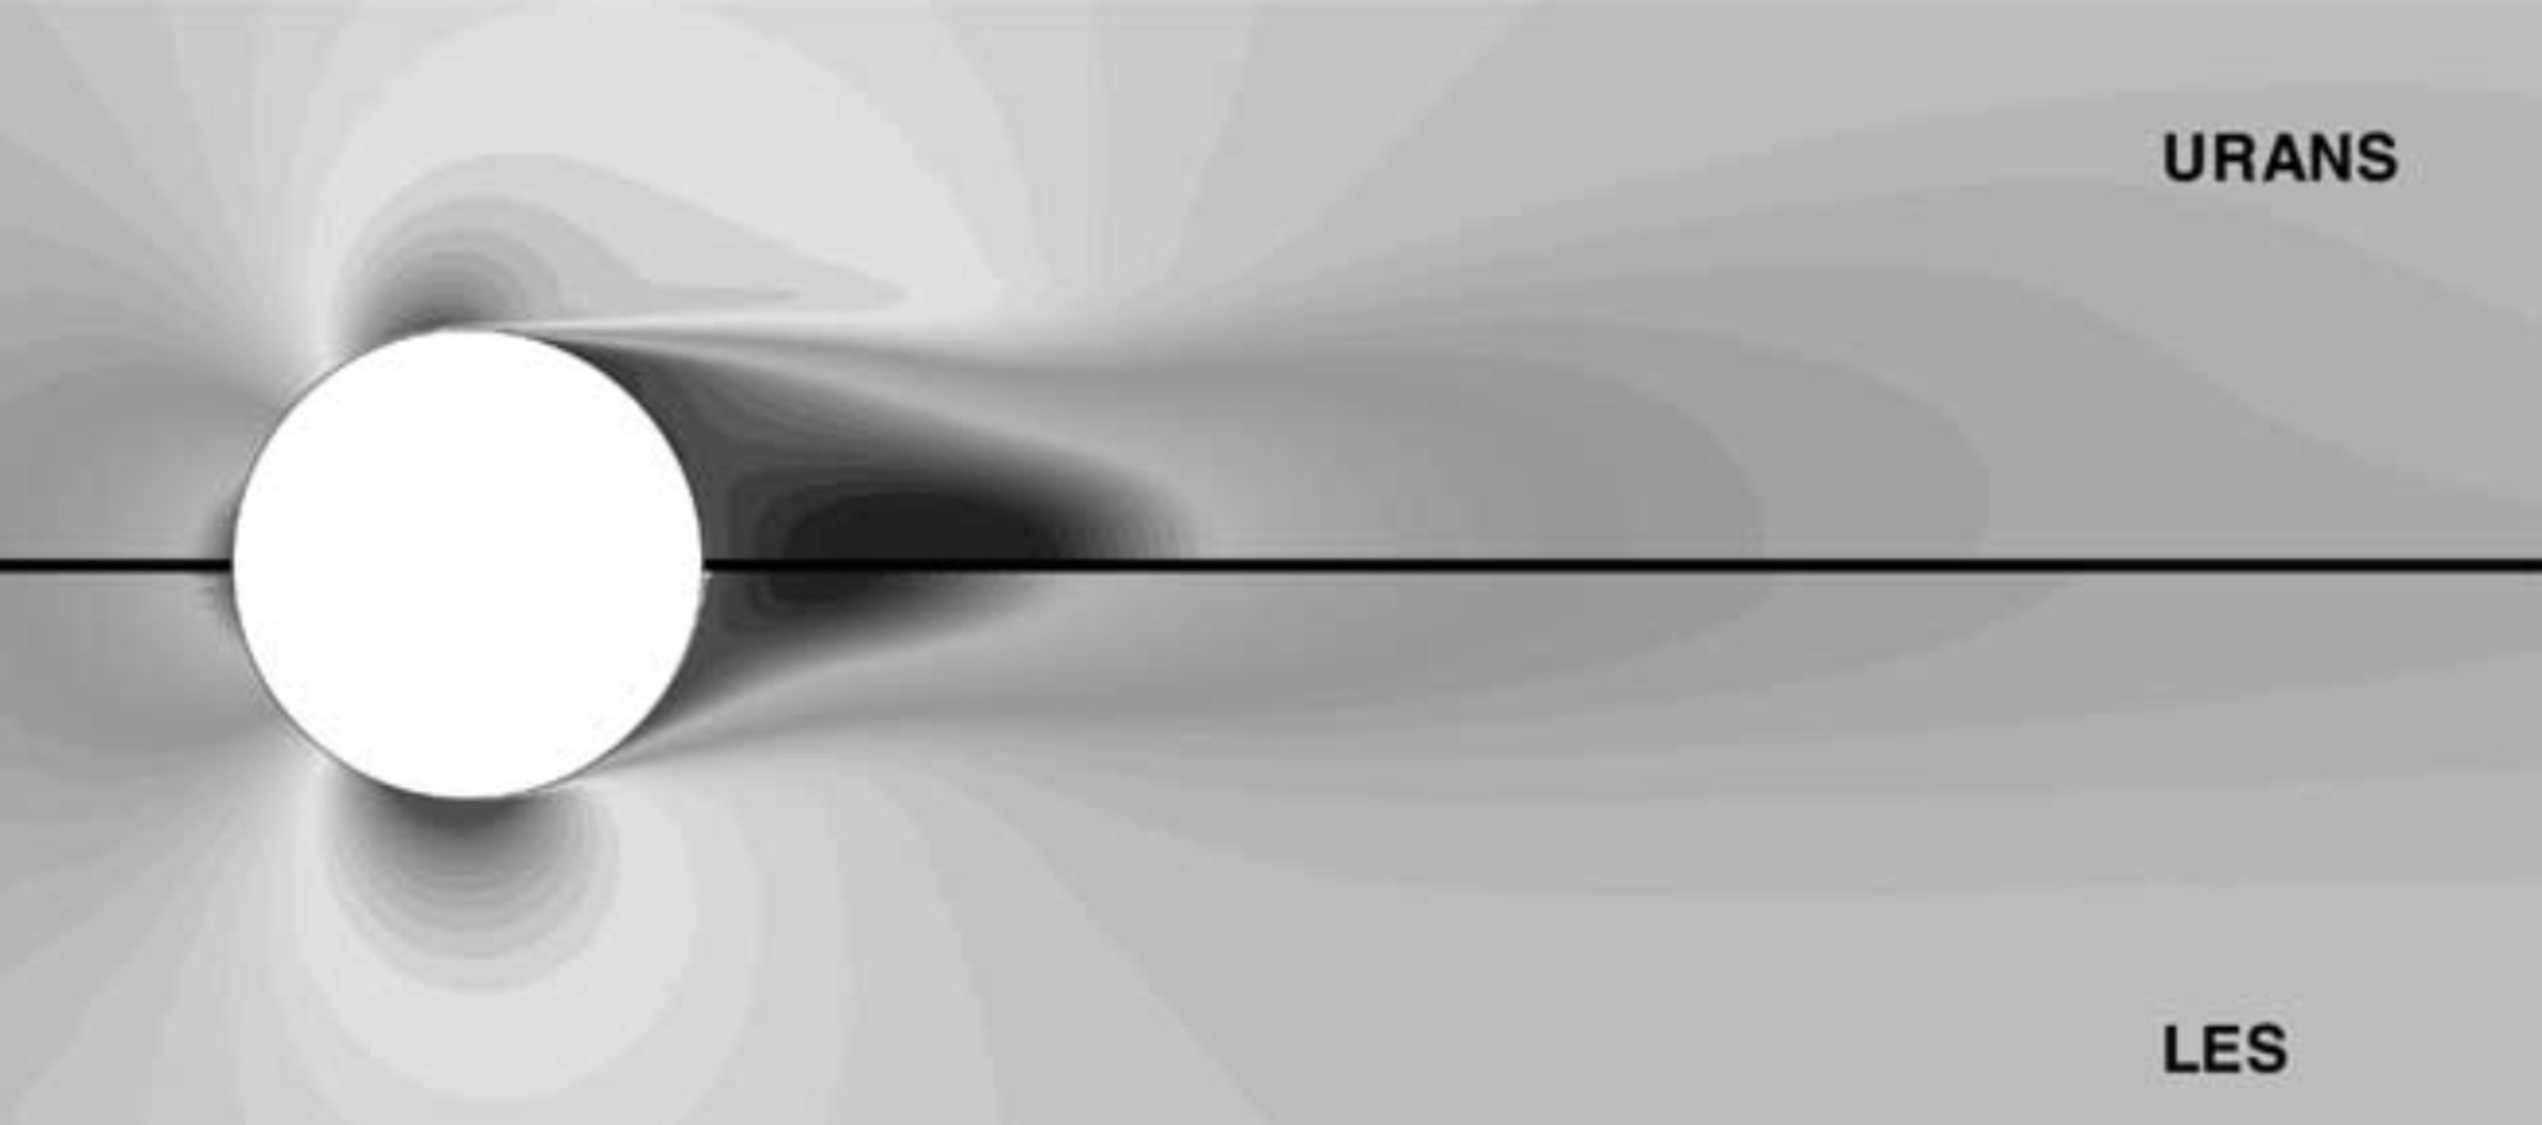
\includegraphics[width=0.5\textwidth]{Images/logan/catalano_2003numerical_SteadyURANSvsLES.pdf}
\caption{ cylinder les vs urans averaged \cite{catalano2003numerical} }
\label{fig:lesvsuranscylinderaveraged}
\end{center}
\end{figure}
%%\vspace{-2em}

Fig. 5. Mean streamwise velocity distribution predicted by LES and URANS. 45 contour levels from U=U1 1⁄4  0:2 to U=U1 1⁄4 1:7 are plotted.

%%% LES VS RANS CYLINDER
%%\vspace{-2em}
% \begin{figure}[htb]
\begin{figure}[H]
\begin{center}
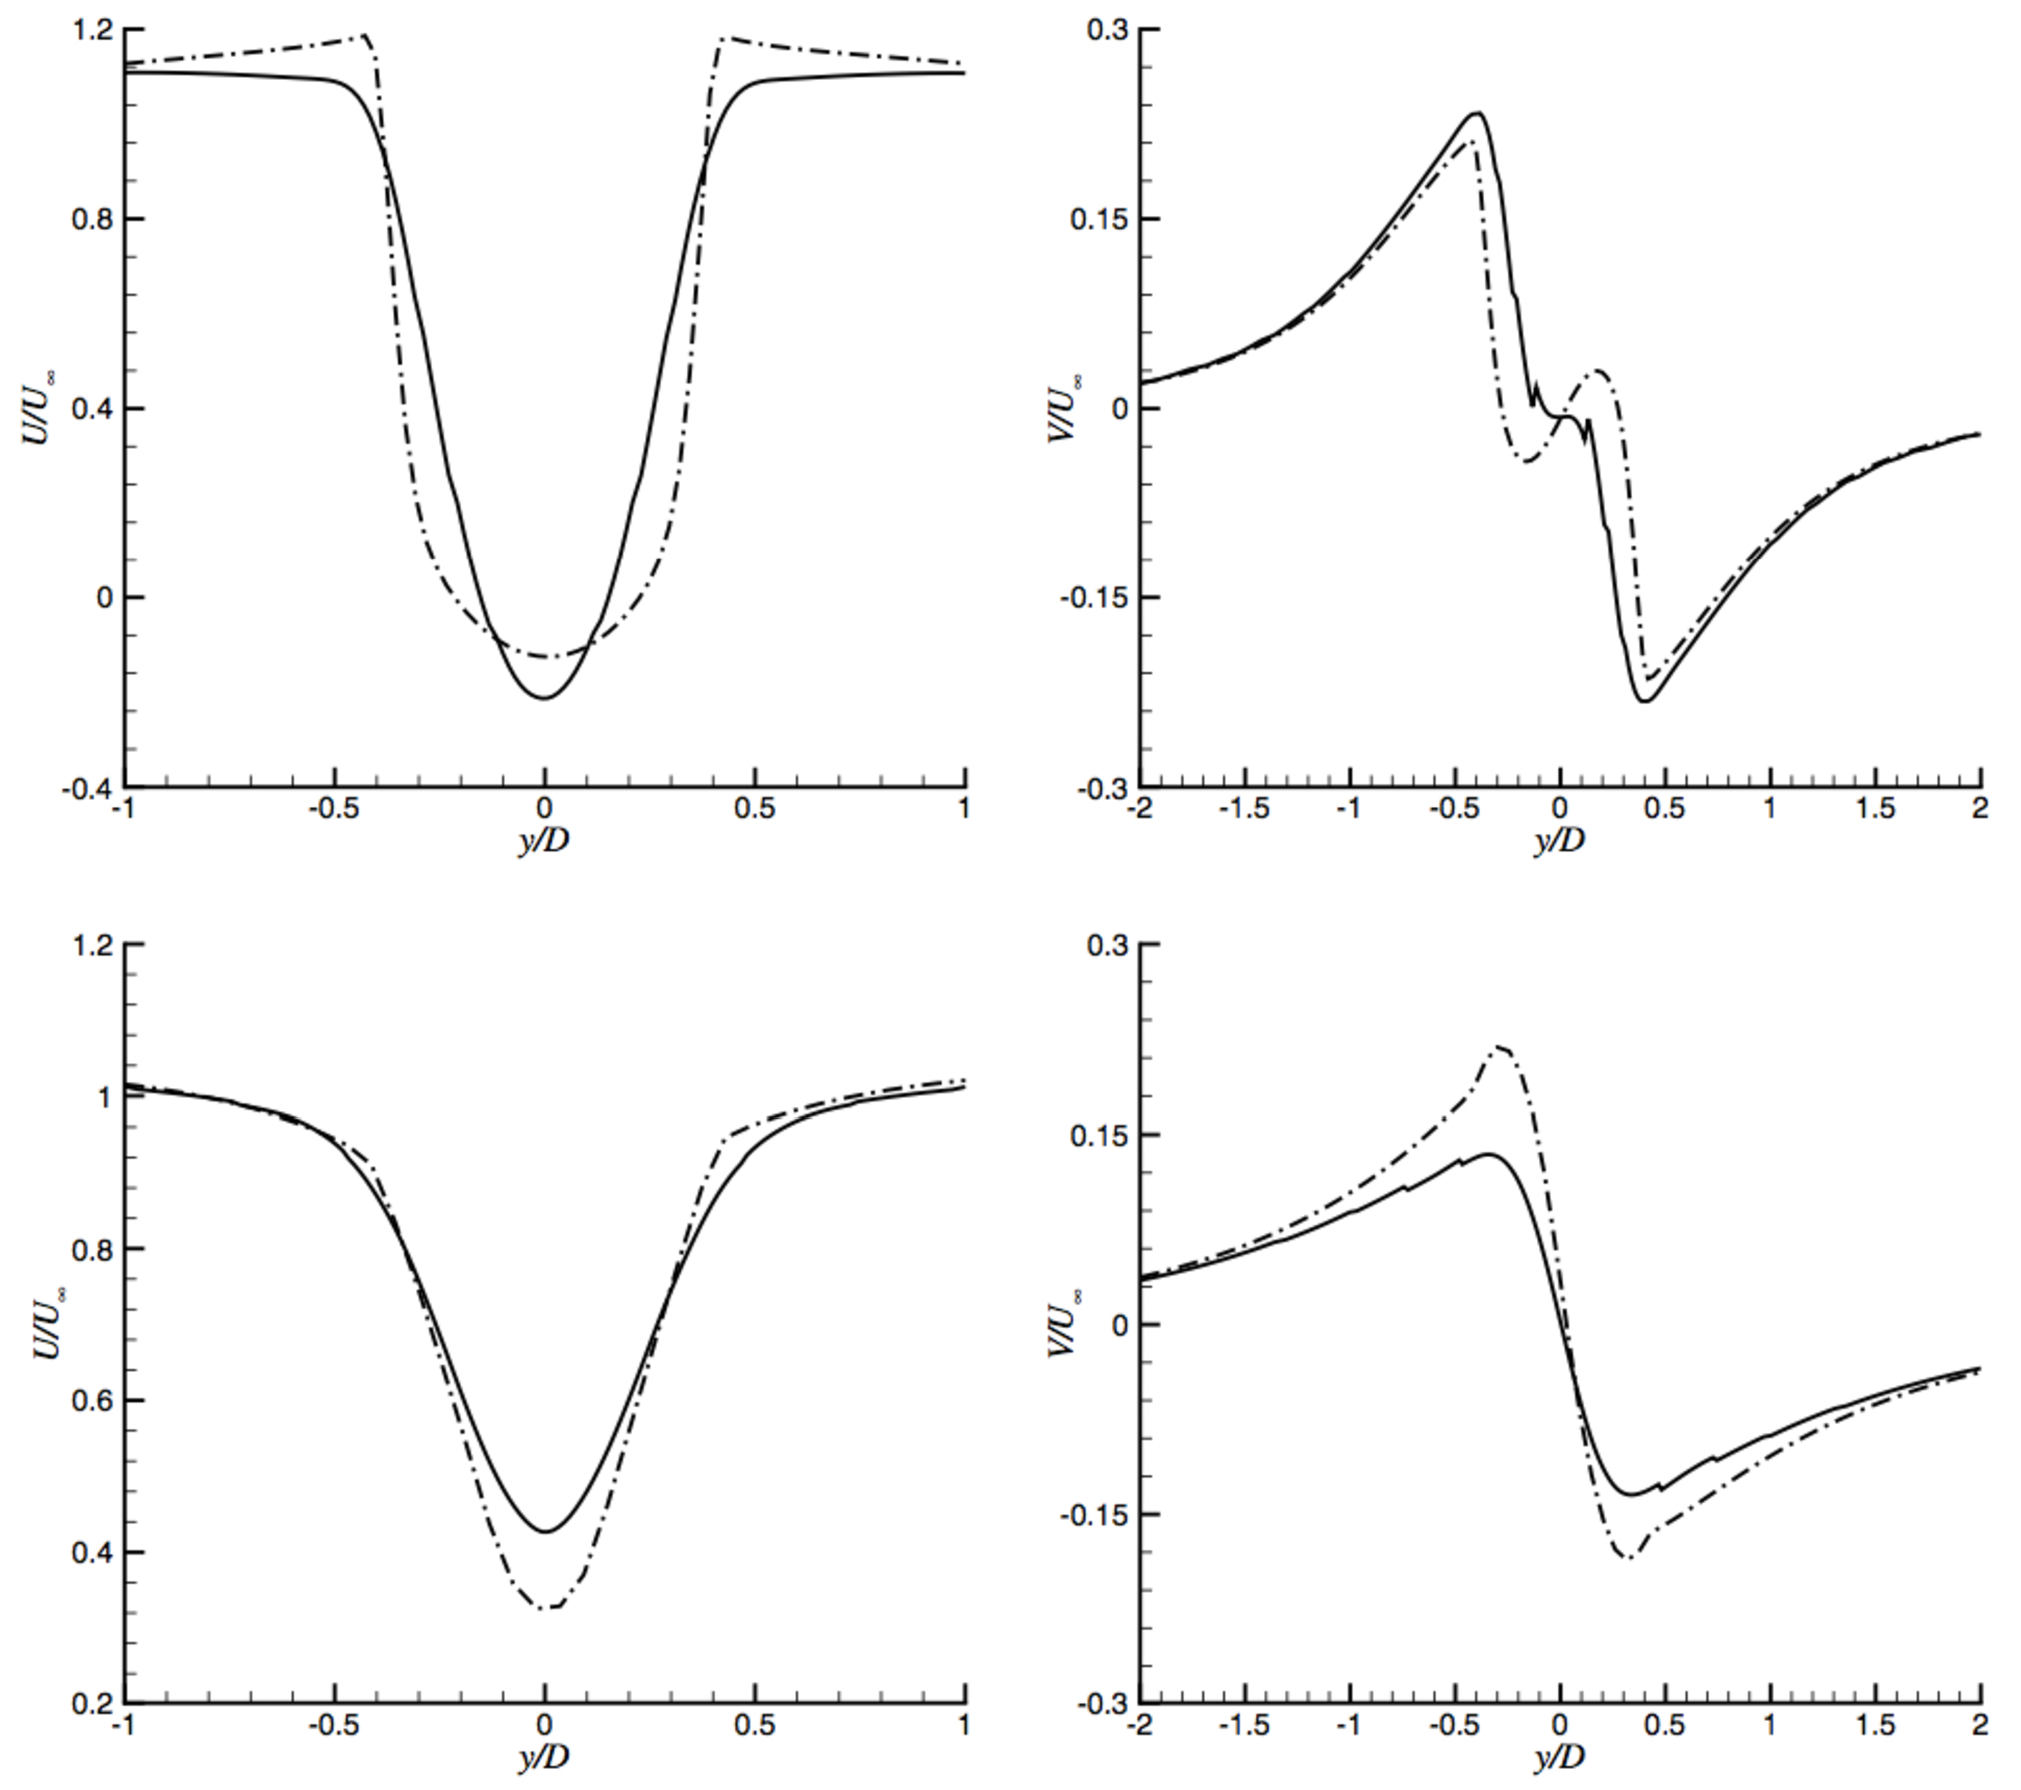
\includegraphics[width=0.5\textwidth]{Images/logan/catalano_2003numerical_VelocityProfiles.pdf}
\caption{ cylinder les vs urans velocity profiles \cite{catalano2003numerical} }
\label{fig:lesvsuranscylindervelprofile}
\end{center}
\end{figure}
%%\vspace{-2em}

Fig. 6. Mean streamwise and vertical velocities at x=D 1⁄4 0:75 (upper figures) and x=D 1⁄4 1:50 (lower figures): (—) LES; (– –) URANS



%%%%%%%%%%%%%%%%%%%%%%%%%%%%%%%%%%%%%%%%%%%%%%%%%%%%%%%%%%%%

%%% LES VS RANS CYLINDER GRID
%%\vspace{-2em}
% \begin{figure}[htb]
\begin{figure}[H]
\begin{center}
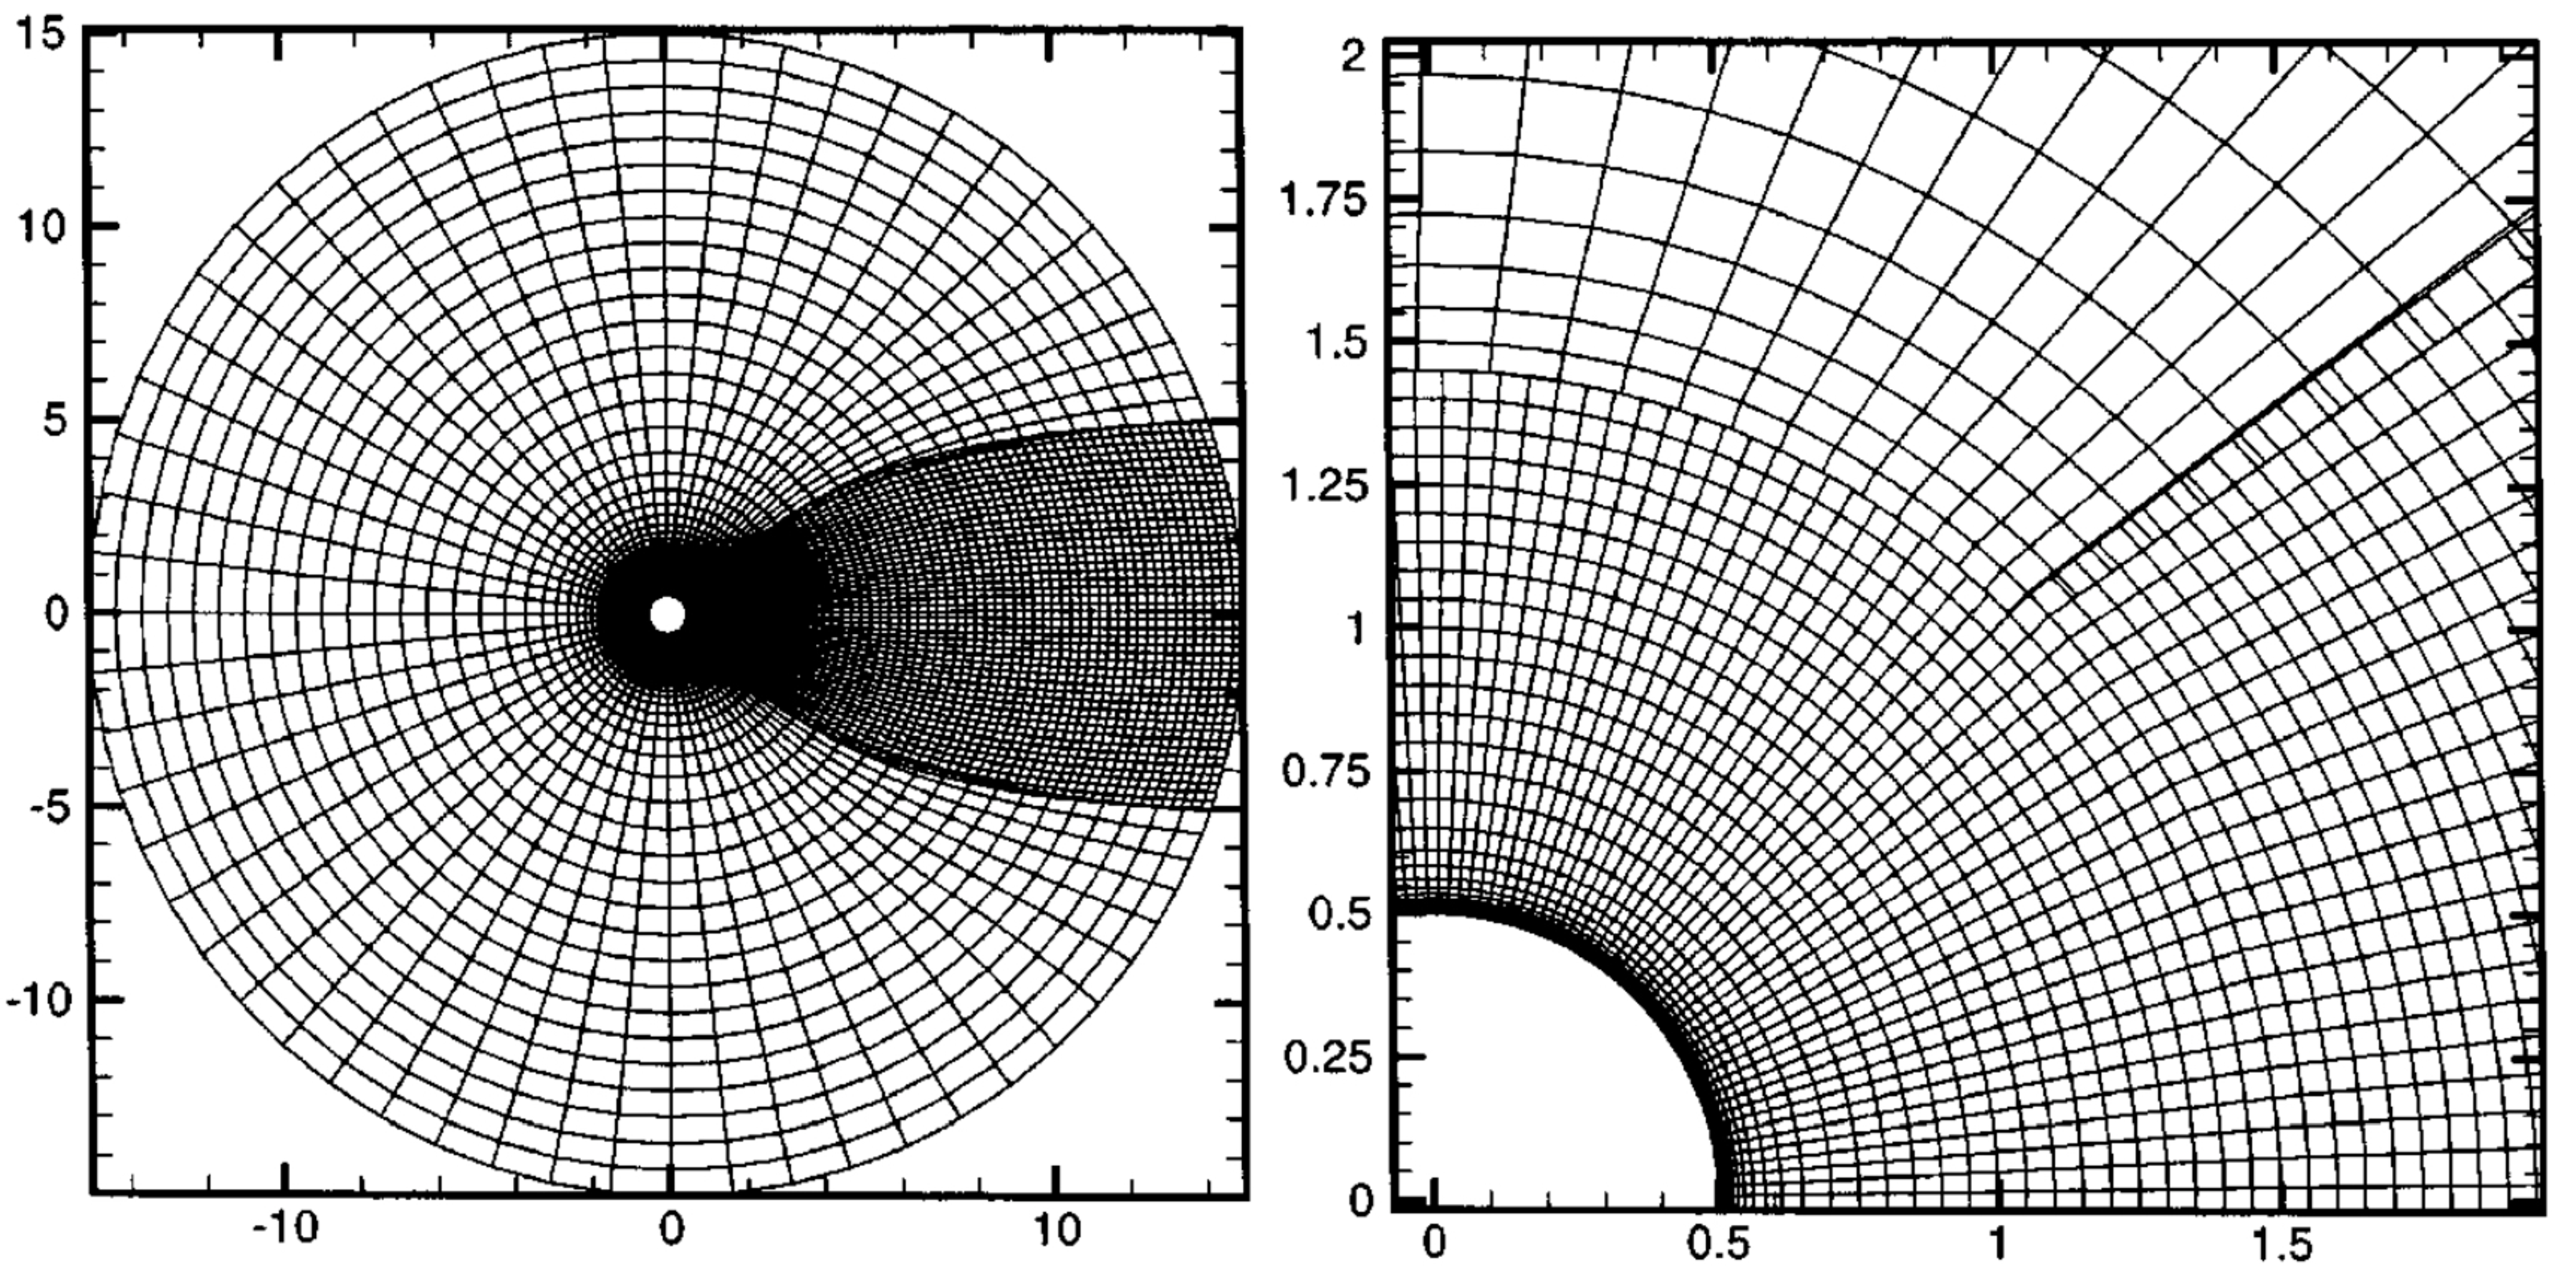
\includegraphics[width=0.5\textwidth]{Images/logan/travin2000detachededdy_grid.pdf}
\caption{ cylinder les vs rans grid \cite{travin2000detachededdy} }
\label{fig:lesvsranscylindergrid}
\end{center}
\end{figure}
%%\vspace{-2em}

Figure1. Medium computational grid, CaseTS2.Innerblock150×36,wakeblock74×36, outer block 59 × 30. The three blocks meet near x = 1.06, y = 1.03.  Grid for spalart cylinders.


%%% LES VS RANS CYLINDER
%%\vspace{-2em}
% \begin{figure}[htb]
\begin{figure}[H]
\begin{center}
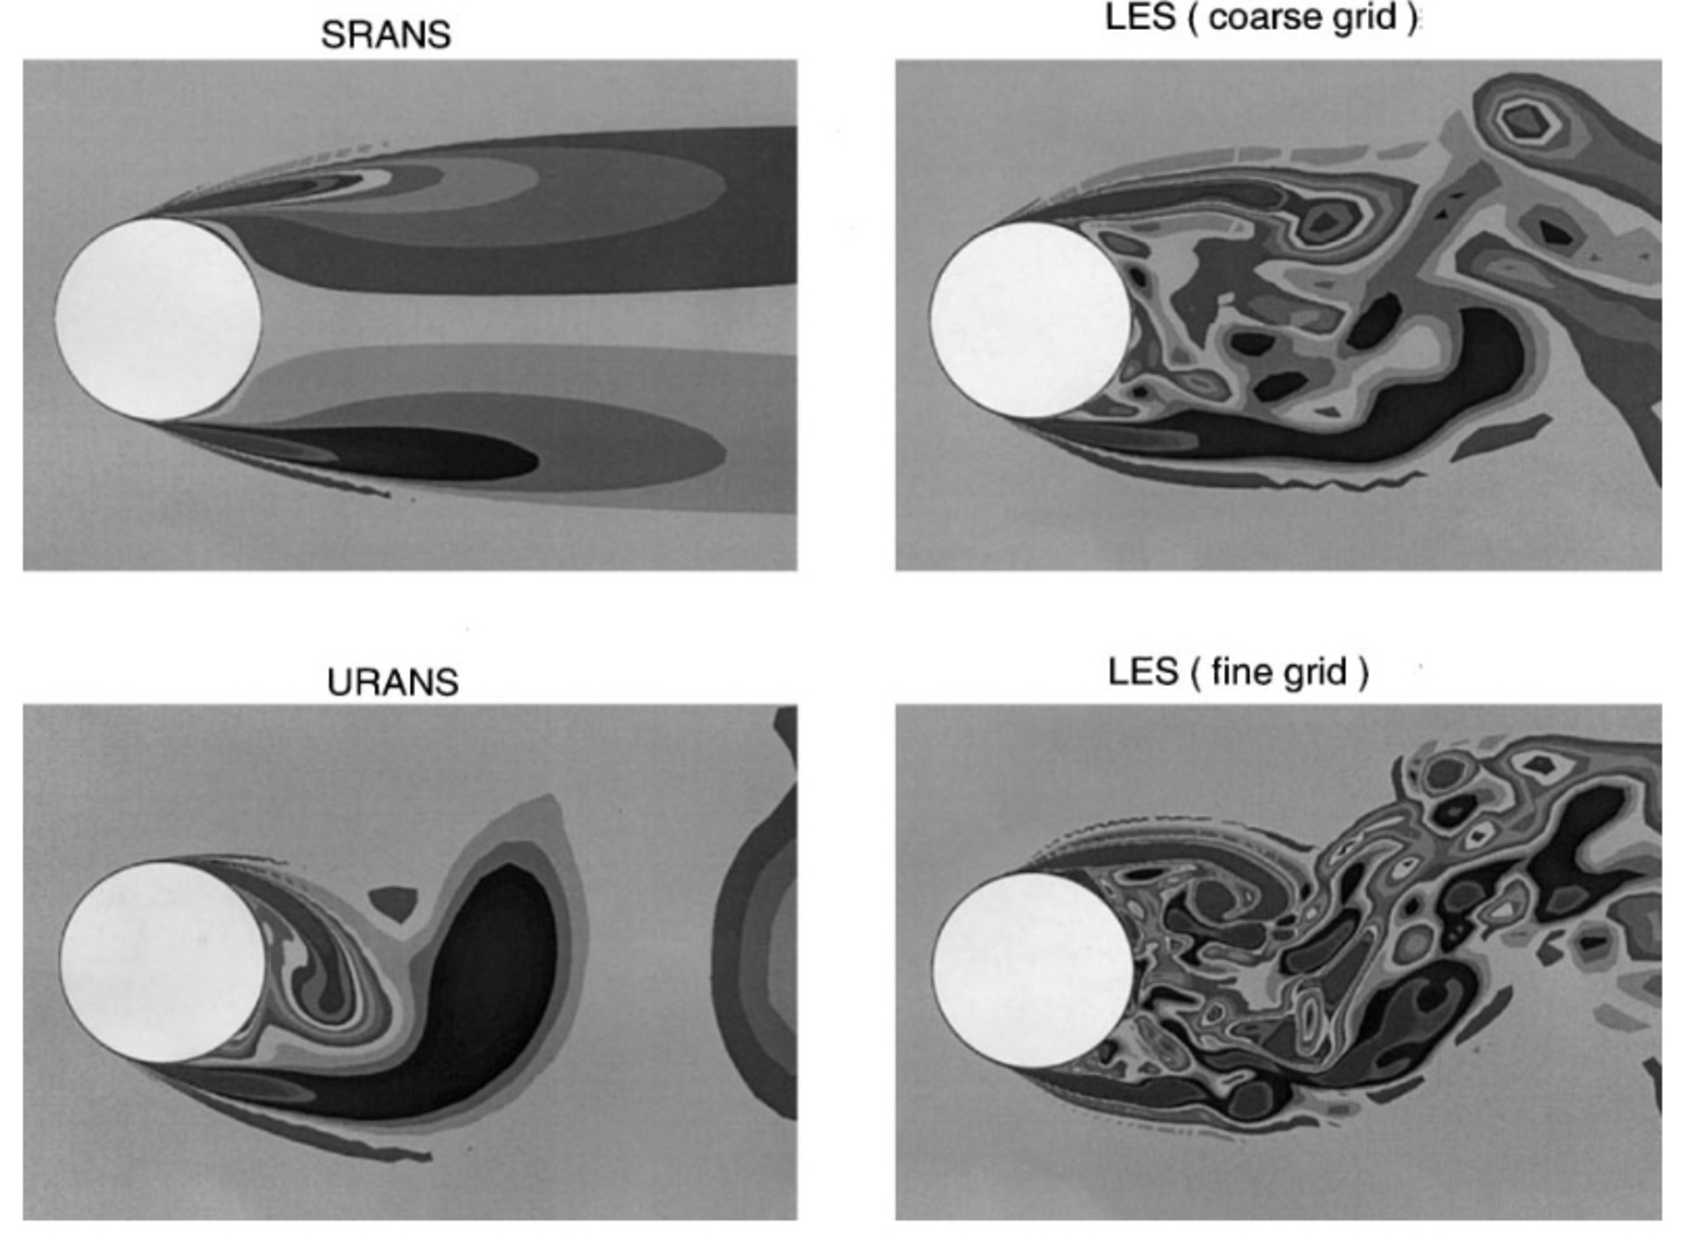
\includegraphics[width=0.5\textwidth]{Images/logan/spalart2000strategies_CylinderLESvsRANS.pdf}
\caption{ cylinder les vs rans \cite{spalart2000strategies} }
\label{fig:lesvsranscylinder}
\end{center}
\end{figure}
%%\vspace{-2em}


grid for LES shown above (actual simulations were DES)




%%% CYLINDER WITH VARIOUS TYPES OF NUMERICAL MODELING
%%\vspace{-2em}
% \begin{figure}[htb]
\begin{figure}[H]
\begin{center}
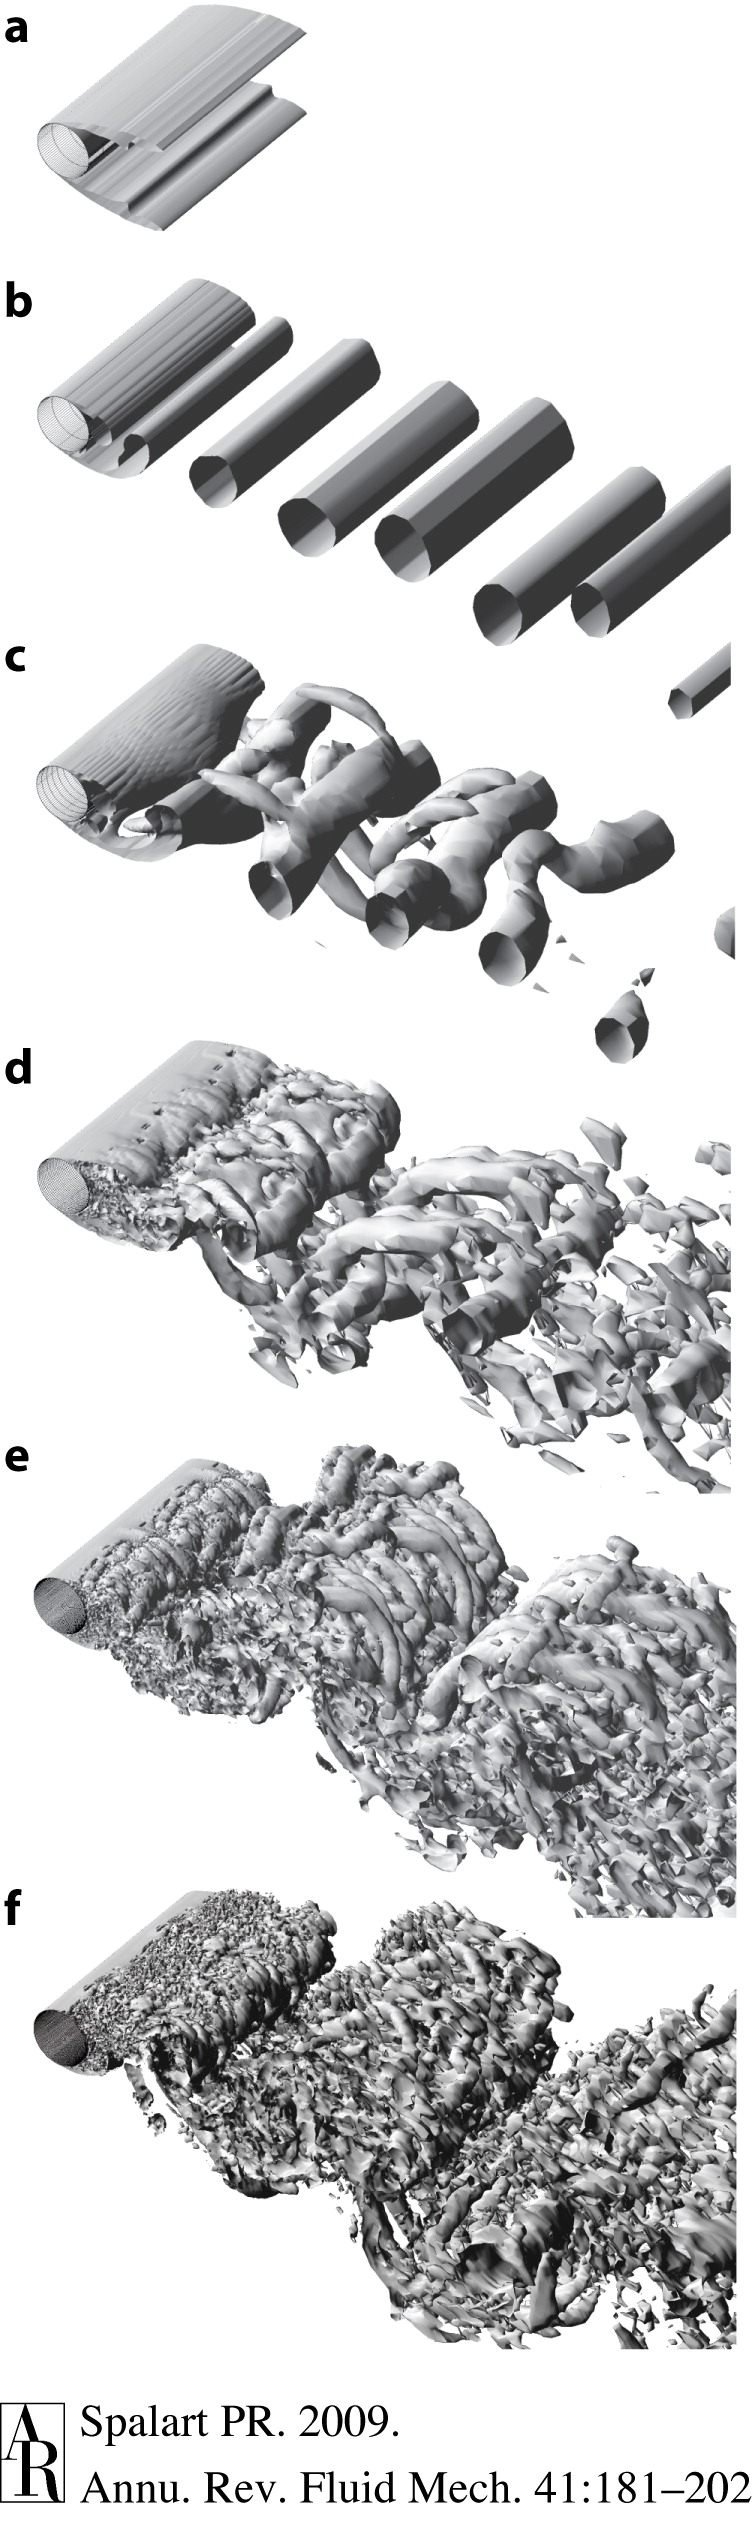
\includegraphics[width=0.3\textwidth]{Images/logan/spalart2009detachededdy_CylinderVariousTurbModels.jpeg}
\caption{ cylinder simulation with RANS, 2DURANS, 3DURANS, SSTDES, SADES \cite{spalart2009detachededdy} }
\label{fig:cylinderturbmodels}
\end{center}
\end{figure}
%%\vspace{-2em}

Vorticity isosurfaces by a circular cylinder: ReD = 5 × 104, laminar separation. Experimental drag
coefficient Cd = 1.15–1.25. (a) Shear-stress transport (SST) turbulence model steady Reynolds-averaged
Navier-Stokes (RANS), Cd = 0.78; (b) SST 2D unsteady RANS, Cd = 1.73; (c) SST 3D unsteady RANS,
Cd = 1.24; (d ) Spalart-Allmaras (SA) detached-eddy simulation (DES), coarse grid, Cd = 1.16; (e) SA DES,
fine grid, Cd = 1.26; ( f ) SST DES, fine grid, Cd = 1.28. Figure courtesy of A. Travin



illustrates the response of DES to grid refinement in its LES region.

DES solutions with different base RANS models are not sensitive to
model choice in the LES region (as opposed to the RANS region, particularly if separation occurs).





%%% DES SPHERE DEMONSTRATING CORRECT TRANSION, COMPARISON TO EXPERIMENT
%%\vspace{-2em}
% \begin{figure}[htb]
\begin{figure}[H]
\begin{center}
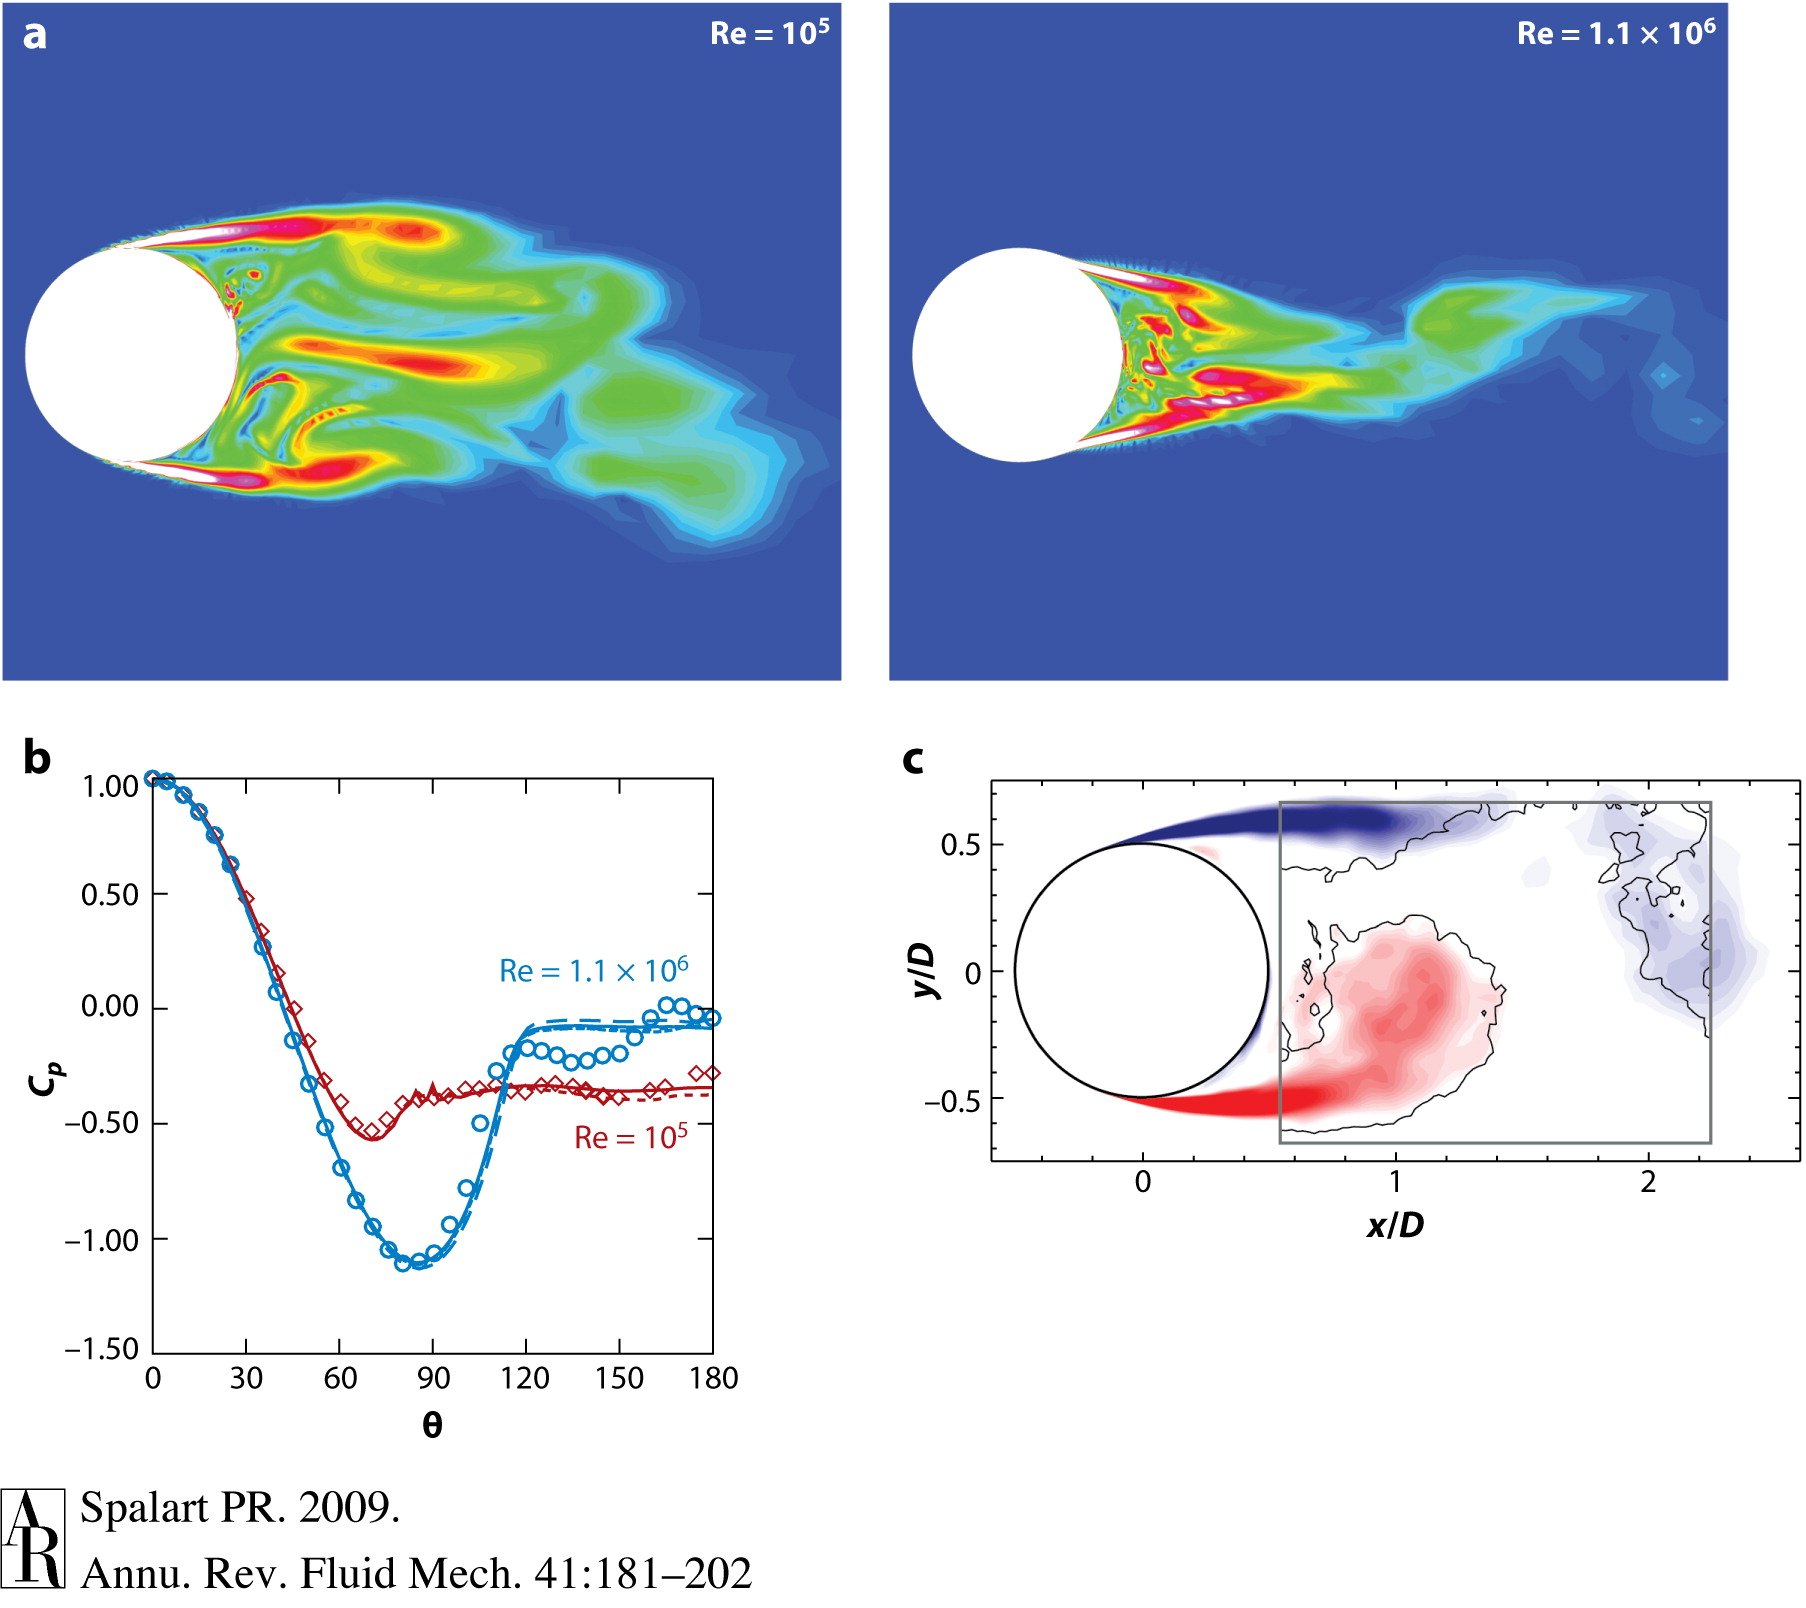
\includegraphics[width=0.6\textwidth]{Images/logan/spalart2009detachededdy_SphereSeparation.jpeg}
\caption{ DES validation from \cite{spalart2009detachededdy}. Sphere transition and drag crisis from \cite{squires2004detachededdy}.  Vorticity validation from \cite{mockett2008demonstration} }
\label{fig:desspherevalidation}
\end{center}
\end{figure}
%%\vspace{-2em}

Simple bluff bodies. (a) Flow visualizations and (b) pressure distributions for a sphere. Re = 105 and 1.1 × 106. Open circles and
diamonds denote experiments, whereas the dotted and dashed lines denote detached-eddy simulation (DES) on two grids. Panels a and
b courtesy of K. Squires. (c) Phase-averaged vorticity contours for a cylinder. Color gradations denote DES conducted by Mockett et al.
(2008), and the solid line denotes experiments by the same authors.

NOTE: DES could be used to emulate the dimples on a golf ball by setting the boundary layer separation point, but true simulation of flow in golf ball dimples requires DNS due to the range of scales




%%% GRID INDUCED SEPARATION FROM DES
%%\vspace{-2em}
% \begin{figure}[htb]
\begin{figure}[H]
\begin{center}
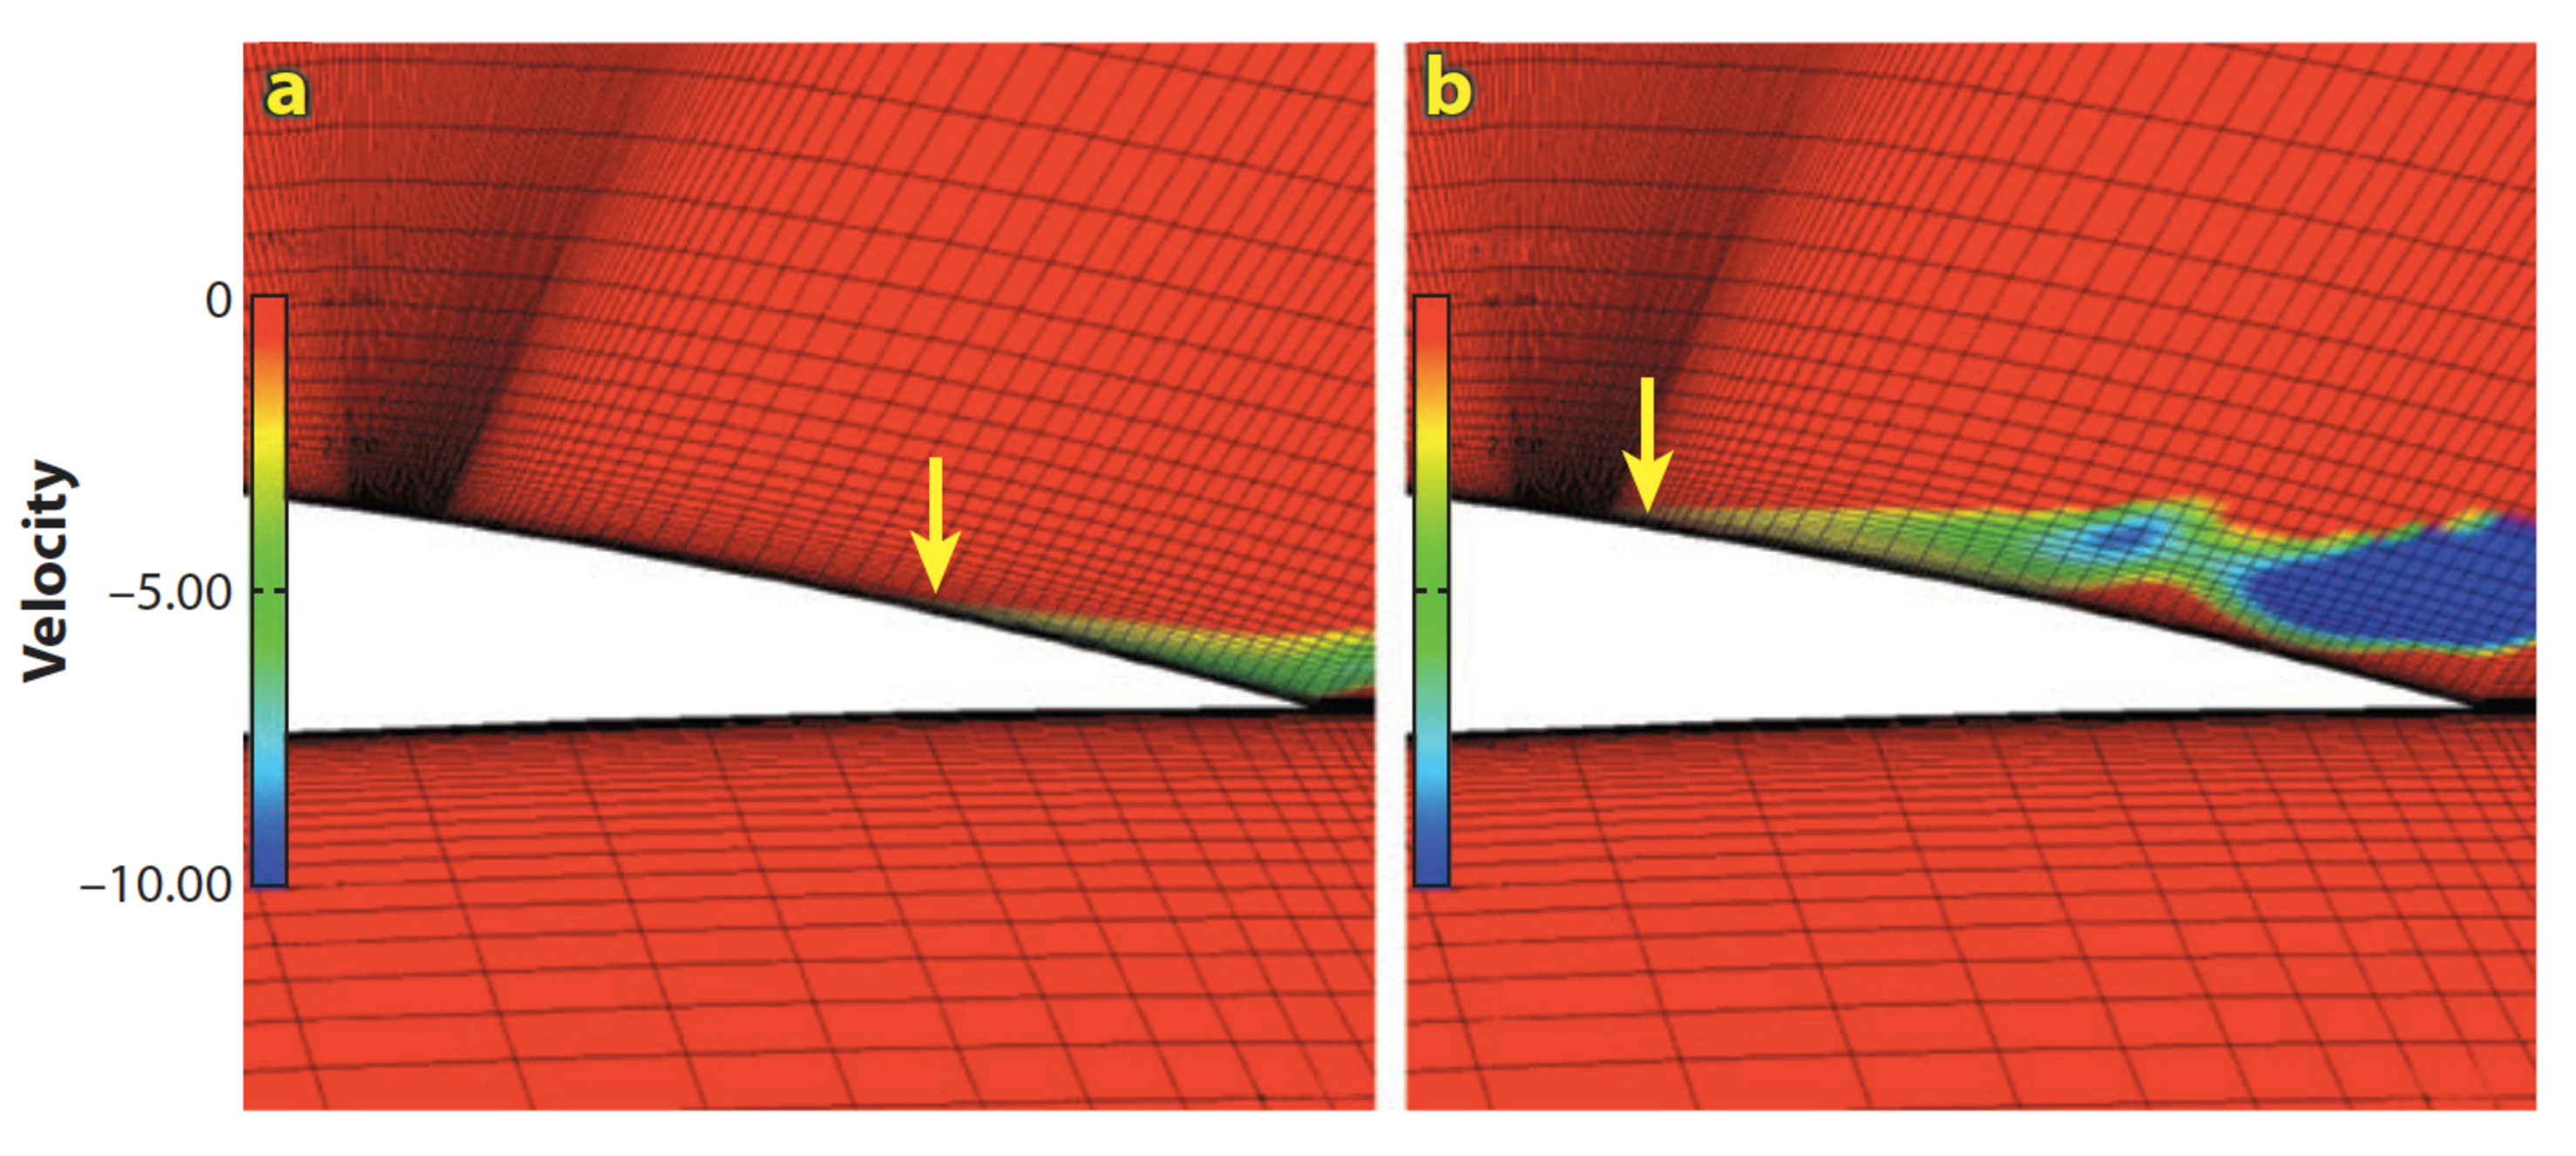
\includegraphics[width=0.6\textwidth]{Images/logan/spalart2009detachededdy_GridInducedSeparation.pdf}
\caption{ Example of DES grid induced separation from \cite{spalart2009detachededdy}, source: \cite{menter2004adaptation} }
\label{fig:desgridinducedseparation}
\end{center}
\end{figure}
%%\vspace{-2em}

Vorticity contours over an airfoil: (a) Reynolds-averaged Navier-Stokes and (b) detached-eddy simulation.
Arrows indicate separation. Figure taken from Menter \& Kuntz 2002.

Potential con of using DES. EXPLAIN HOW GRID INDUCED SEPARATION WORKS.



%%%%%%%%%%%%%%%%%%%%%%%%%%%%%%%%%%%%%%%%%%%%%%%%%%%%%%%%%%%%

%%% F15 DES
%%\vspace{-2em}
% \begin{figure}[htb]
\begin{figure}[H]
\begin{center}
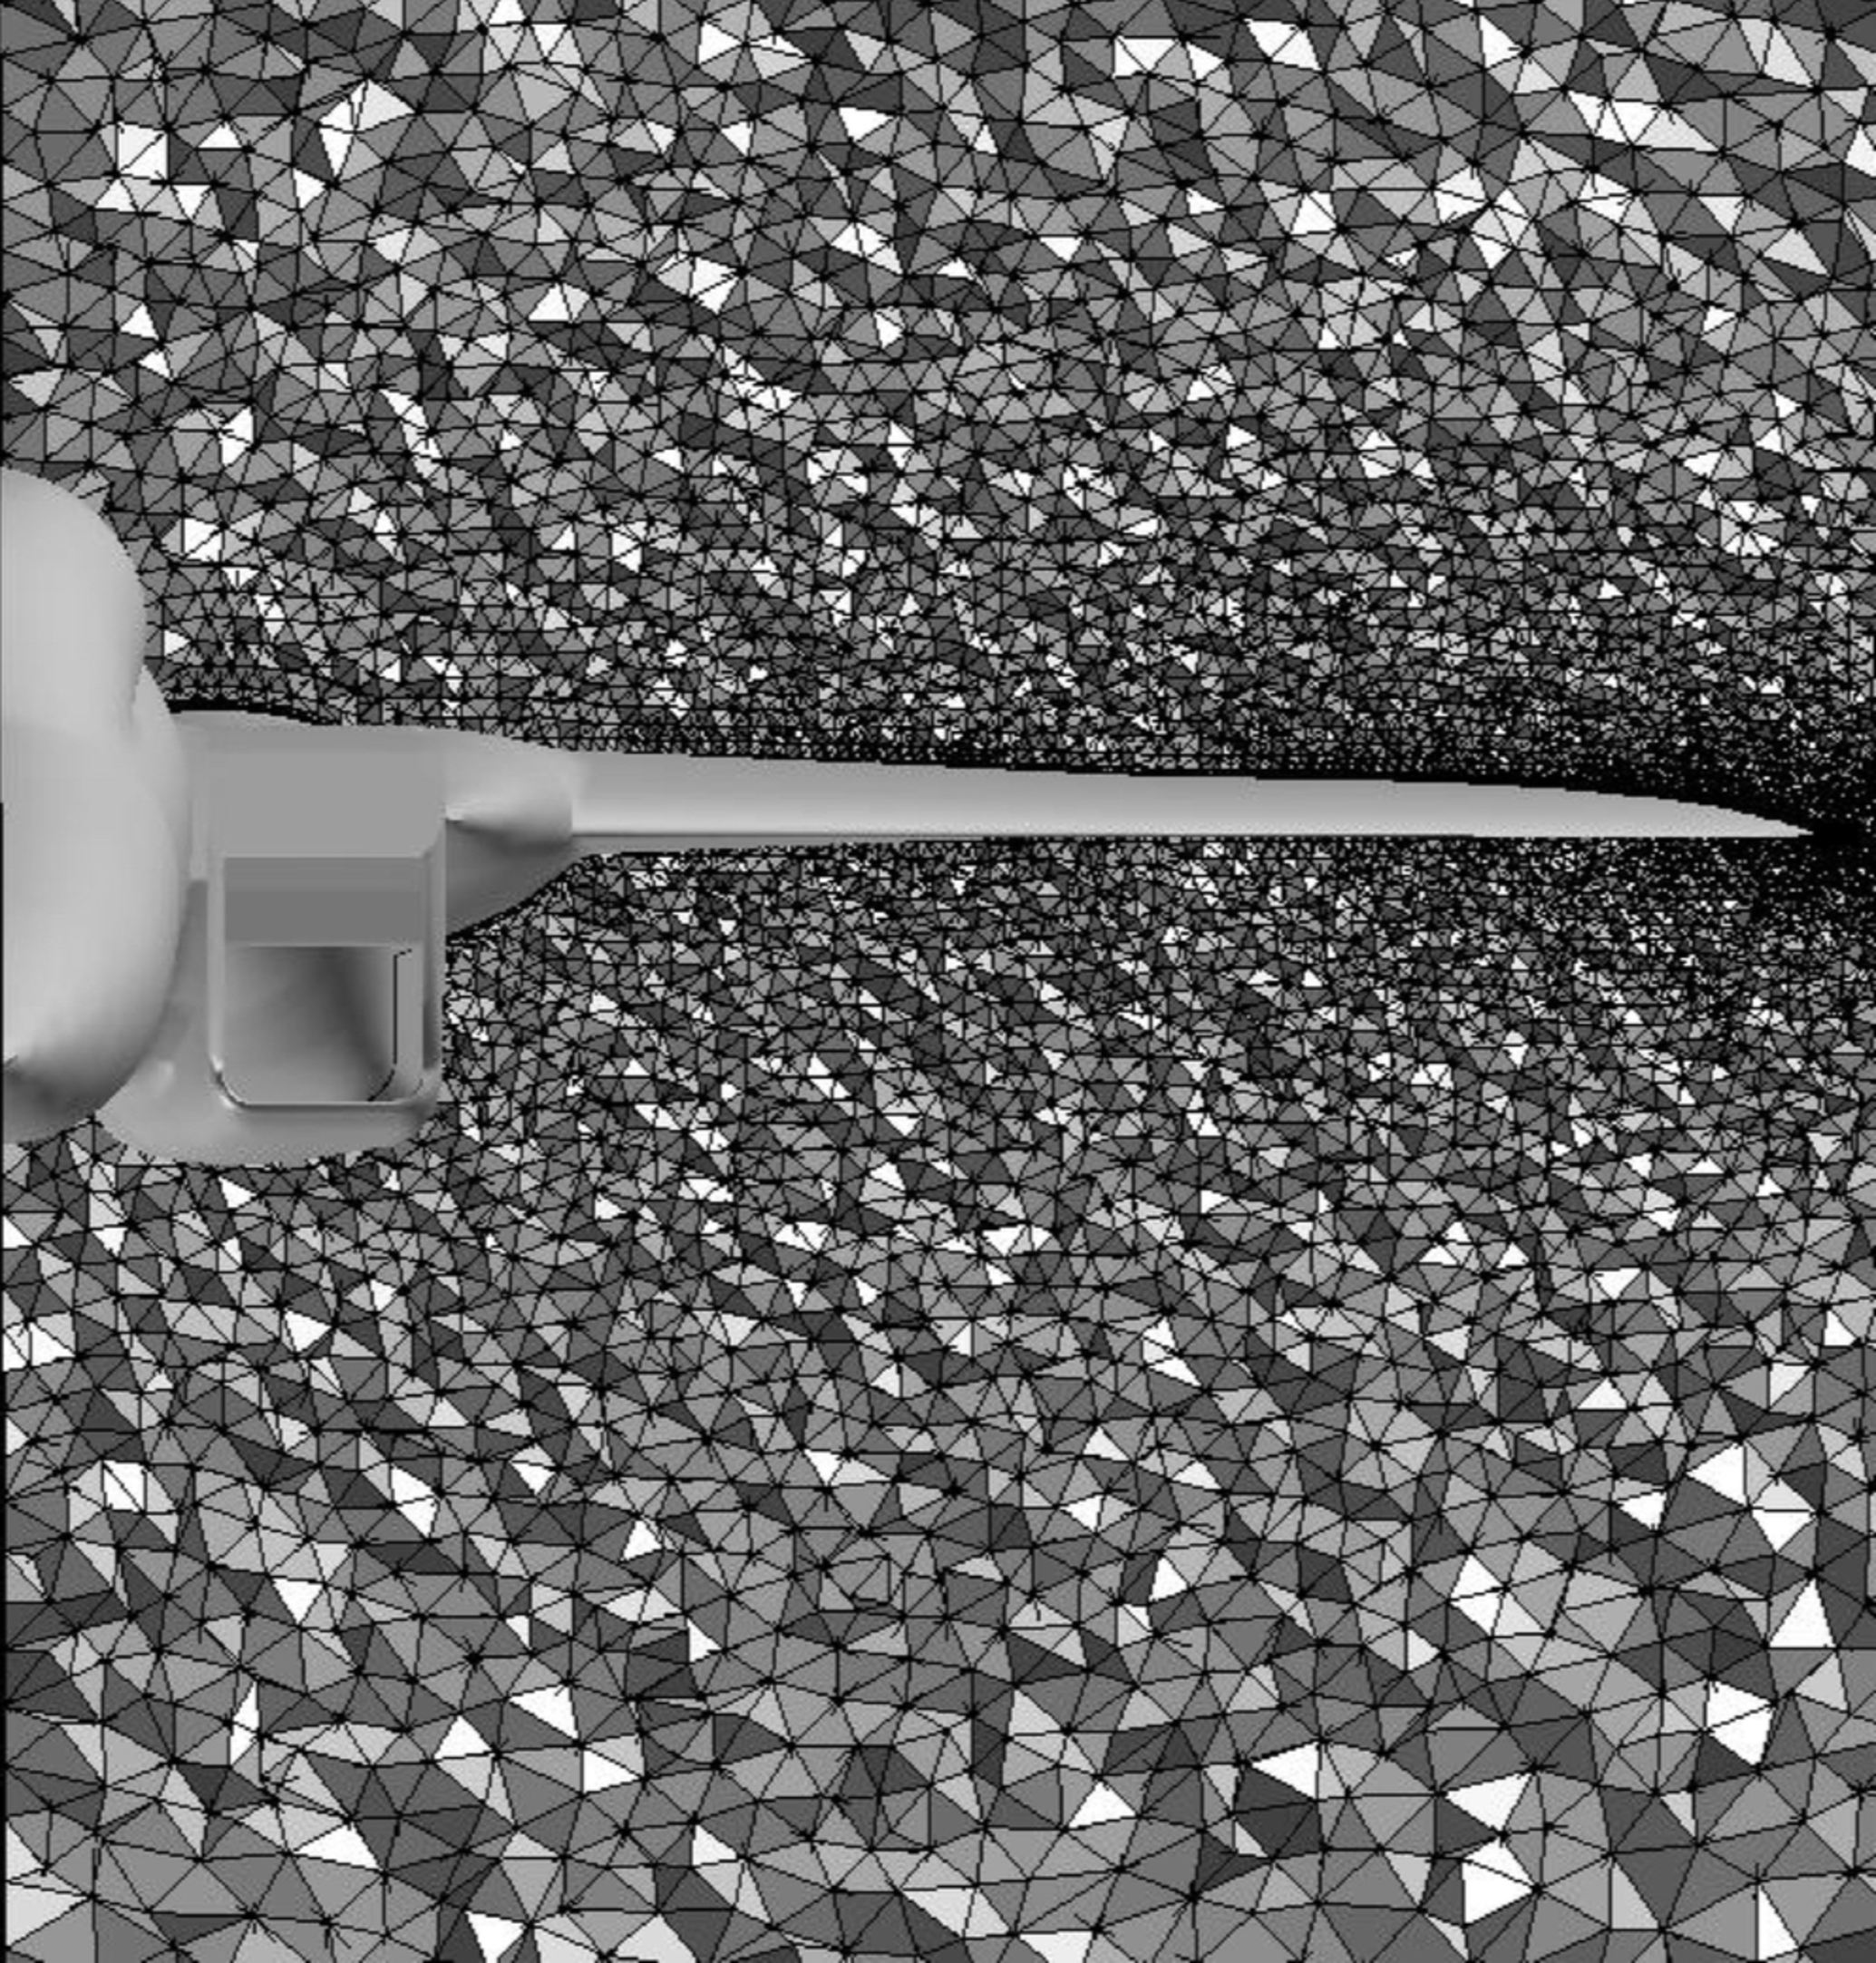
\includegraphics[width=0.45\textwidth]{Images/logan/forsythe2004detachededdy_f15grid.pdf}
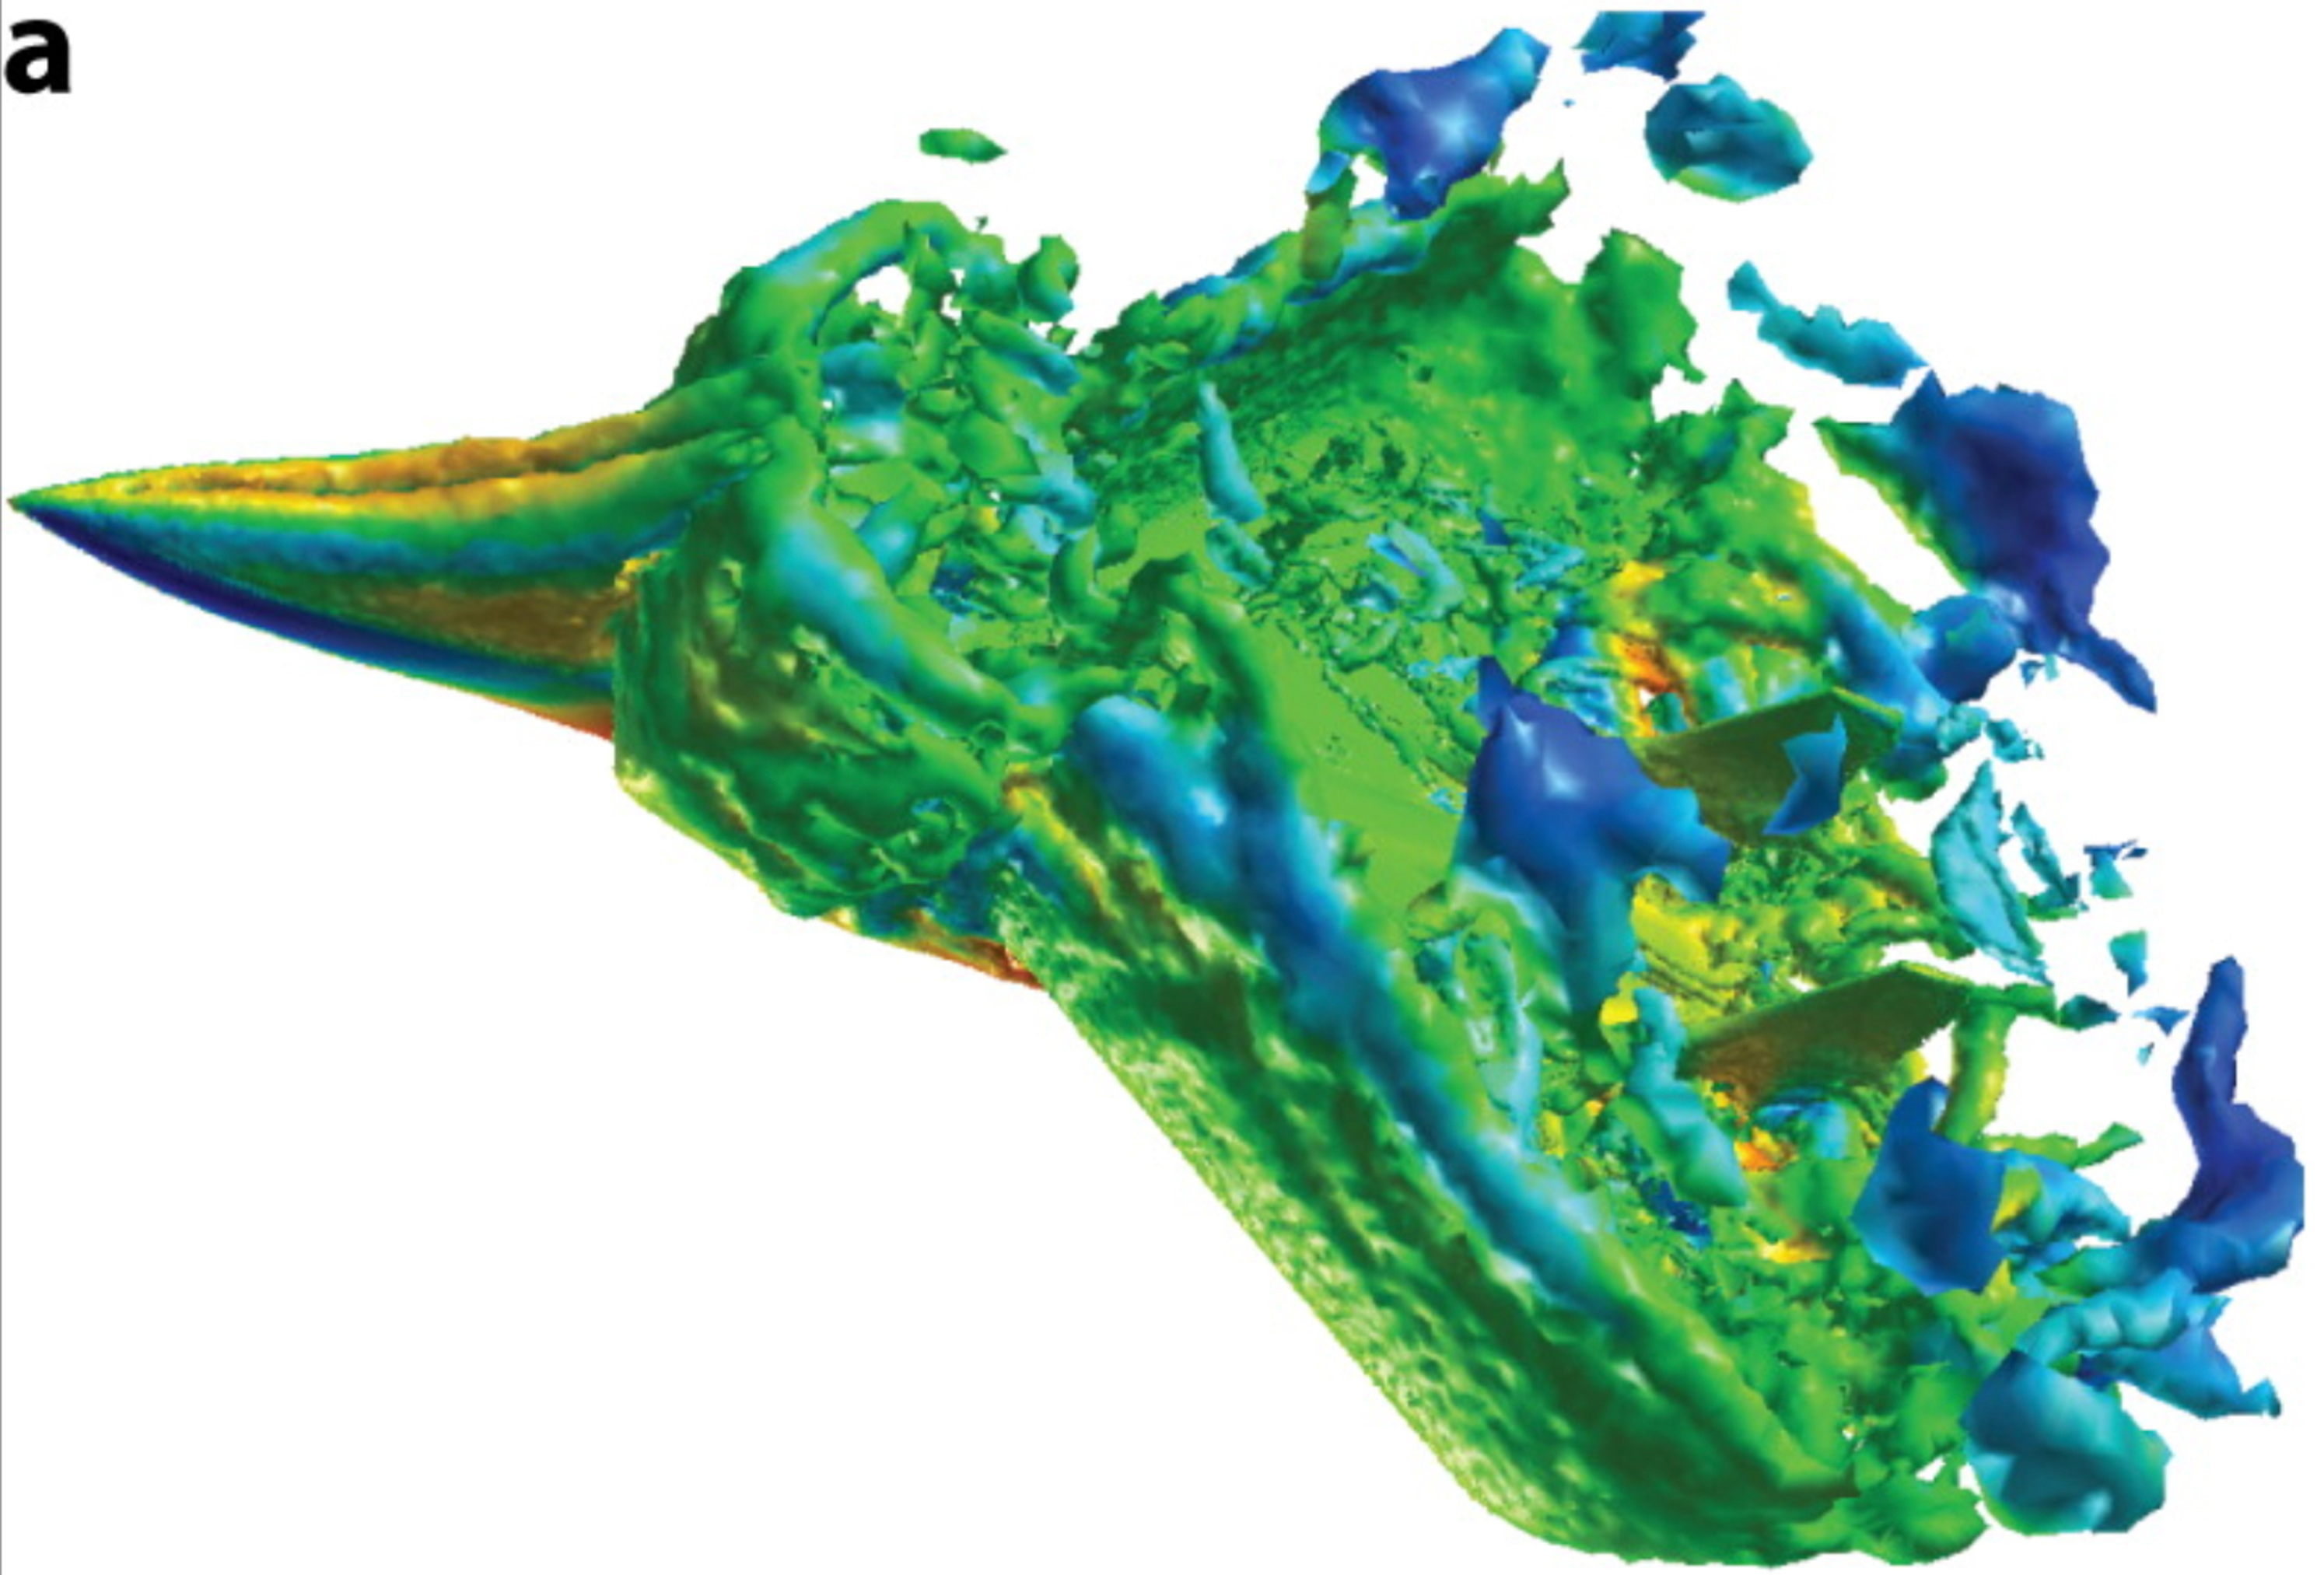
\includegraphics[width=0.45\textwidth]{Images/logan/spalart2009detachededdy_f15des.pdf}
\caption{ F-15 DES grid (left) \cite{forsythe2004detachededdy} vorticity isocontours (right) \cite{spalart2009detachededdy} }
\label{fig:f15des}
\end{center}
\end{figure}
%%\vspace{-2em}



%%% CAR DES
%%\vspace{-2em}
% \begin{figure}[htb]
\begin{figure}[H]
\begin{center}
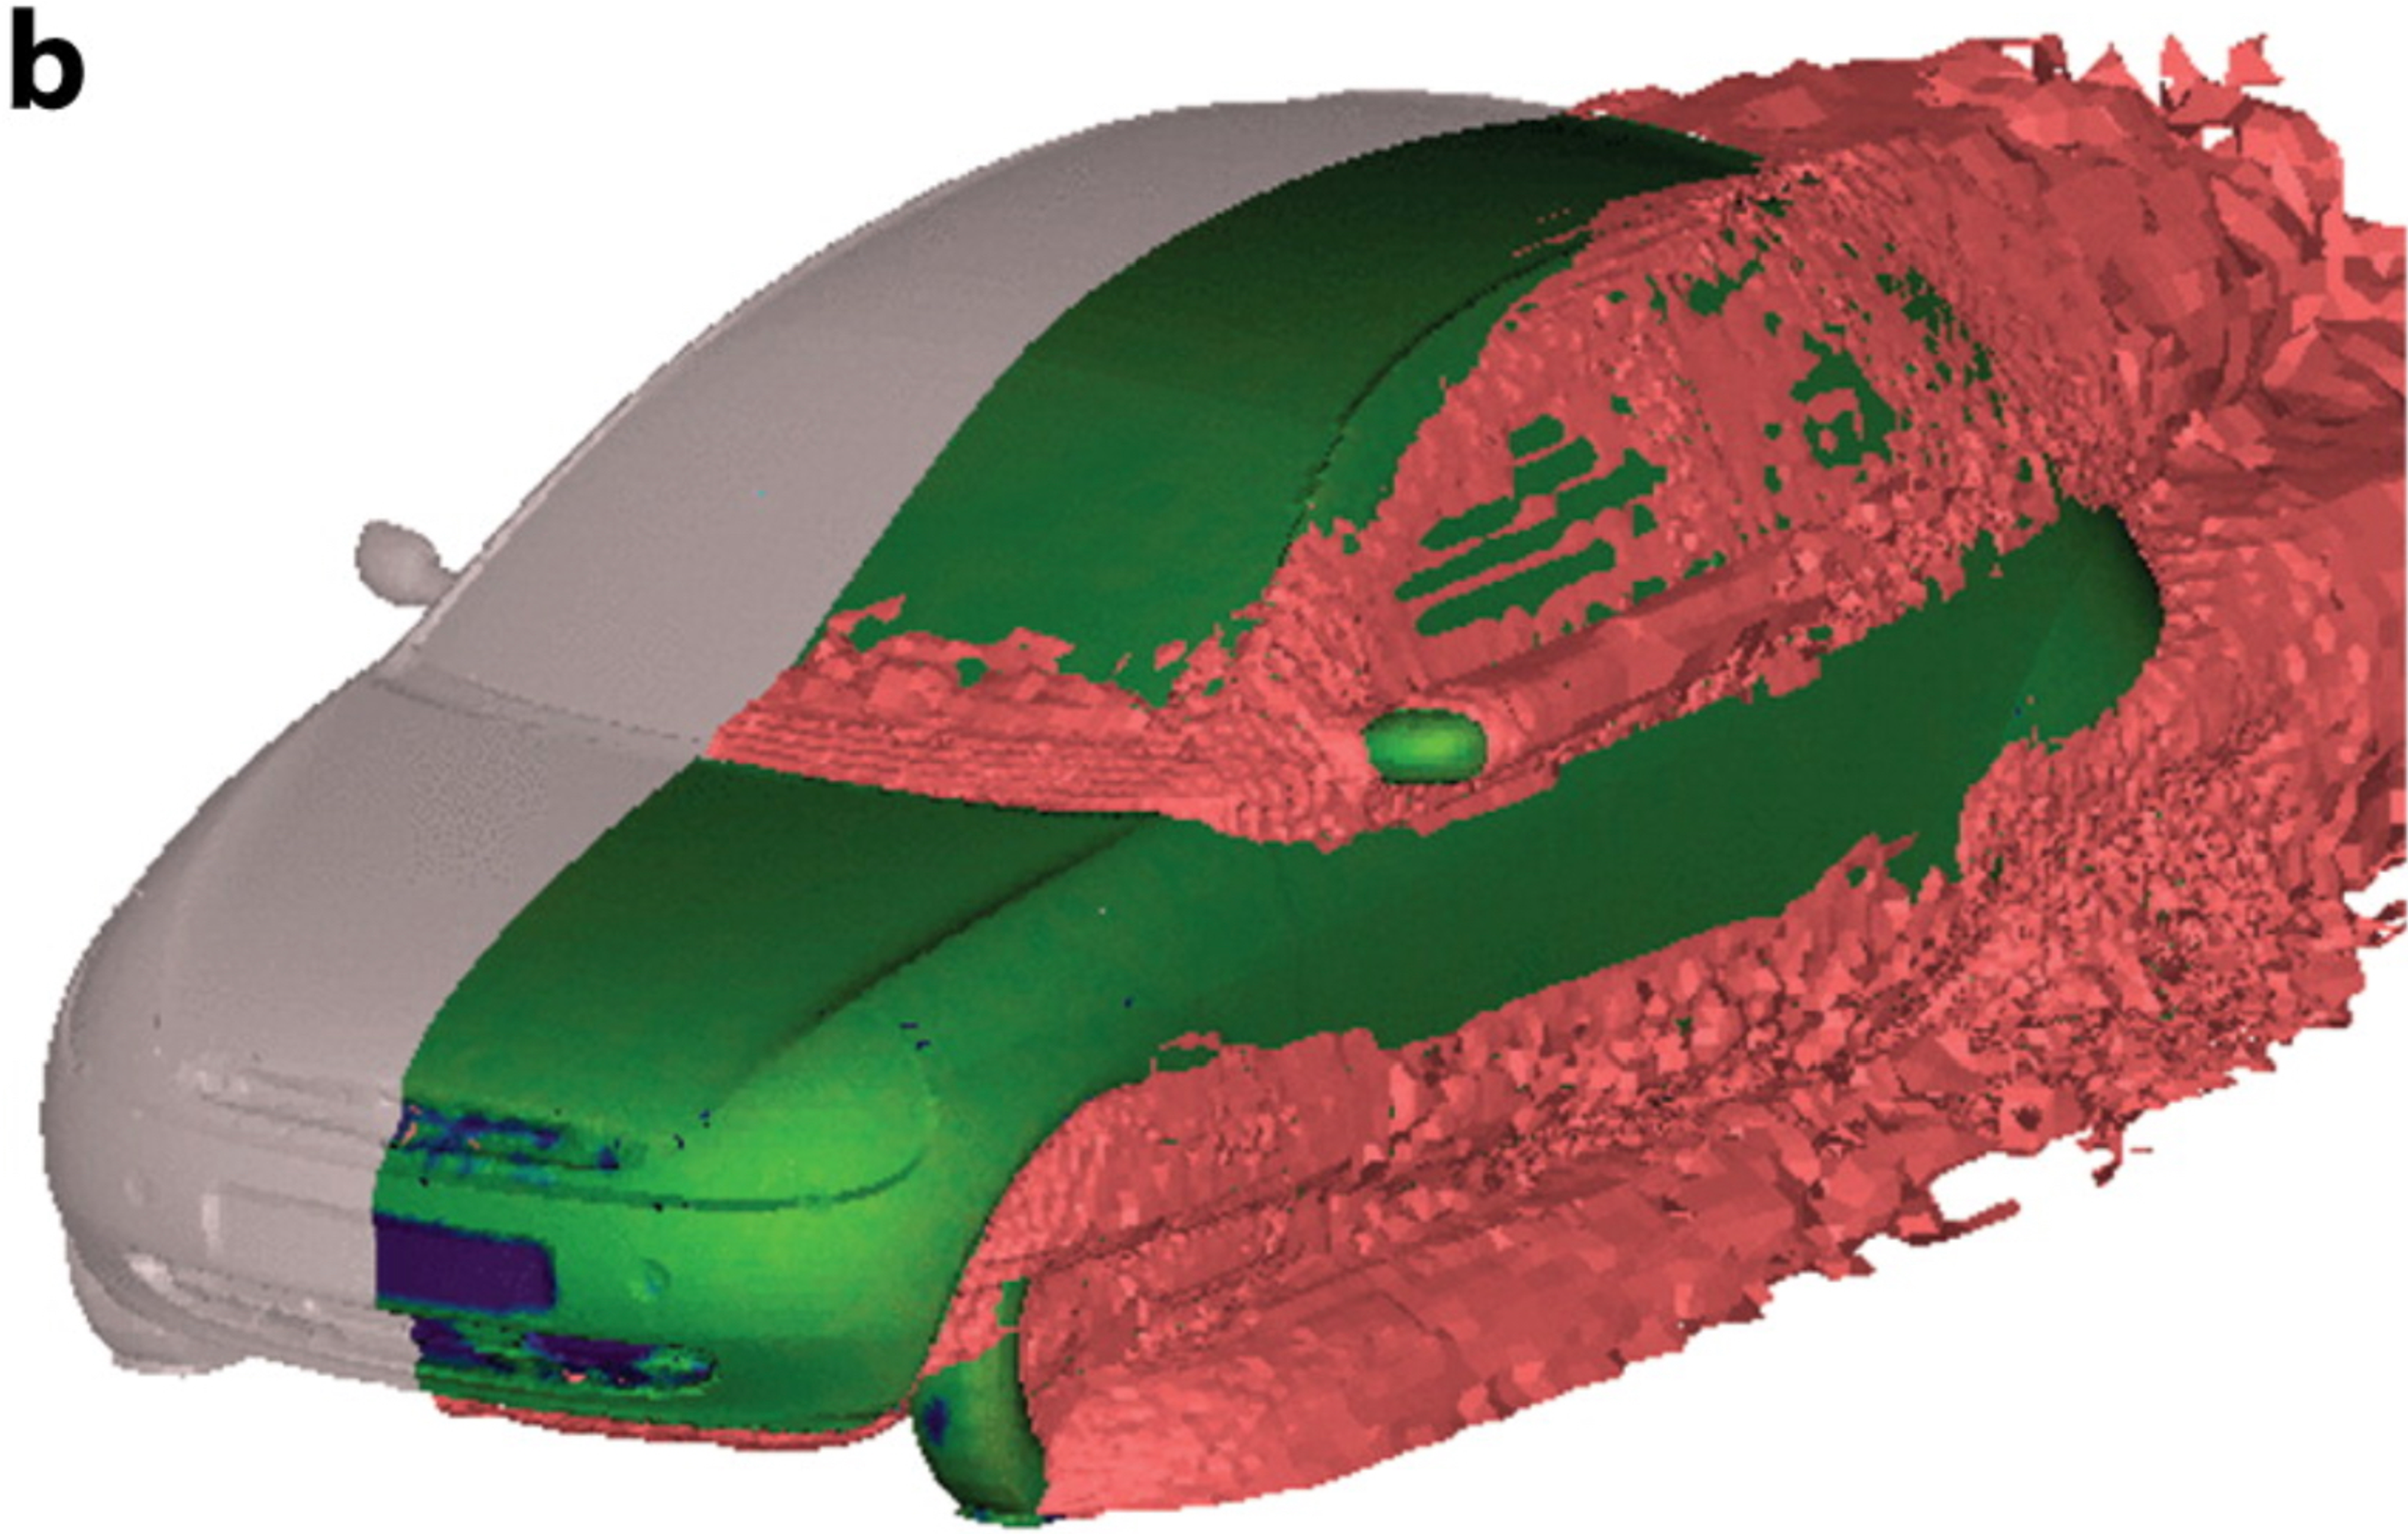
\includegraphics[width=0.5\textwidth]{Images/logan/spalart2009detachededdy_carDES.pdf}
\caption{ car DES isocontours \cite{mendonca2002towards} }
\label{fig:cardes}
\end{center}
\end{figure}
%%\vspace{-2em}









%%%%%%%%%%%%%%%%%%%%%%%%%%%%%%%%%%%%%%%%%%%%%%%%%%%%%%%%%%%%


%%% CURVE BACKSTEP VELOCITY PROFILE LES VS RANS
%%\vspace{-2em}
% \begin{figure}[htb]
\begin{figure}[H]
\begin{center}
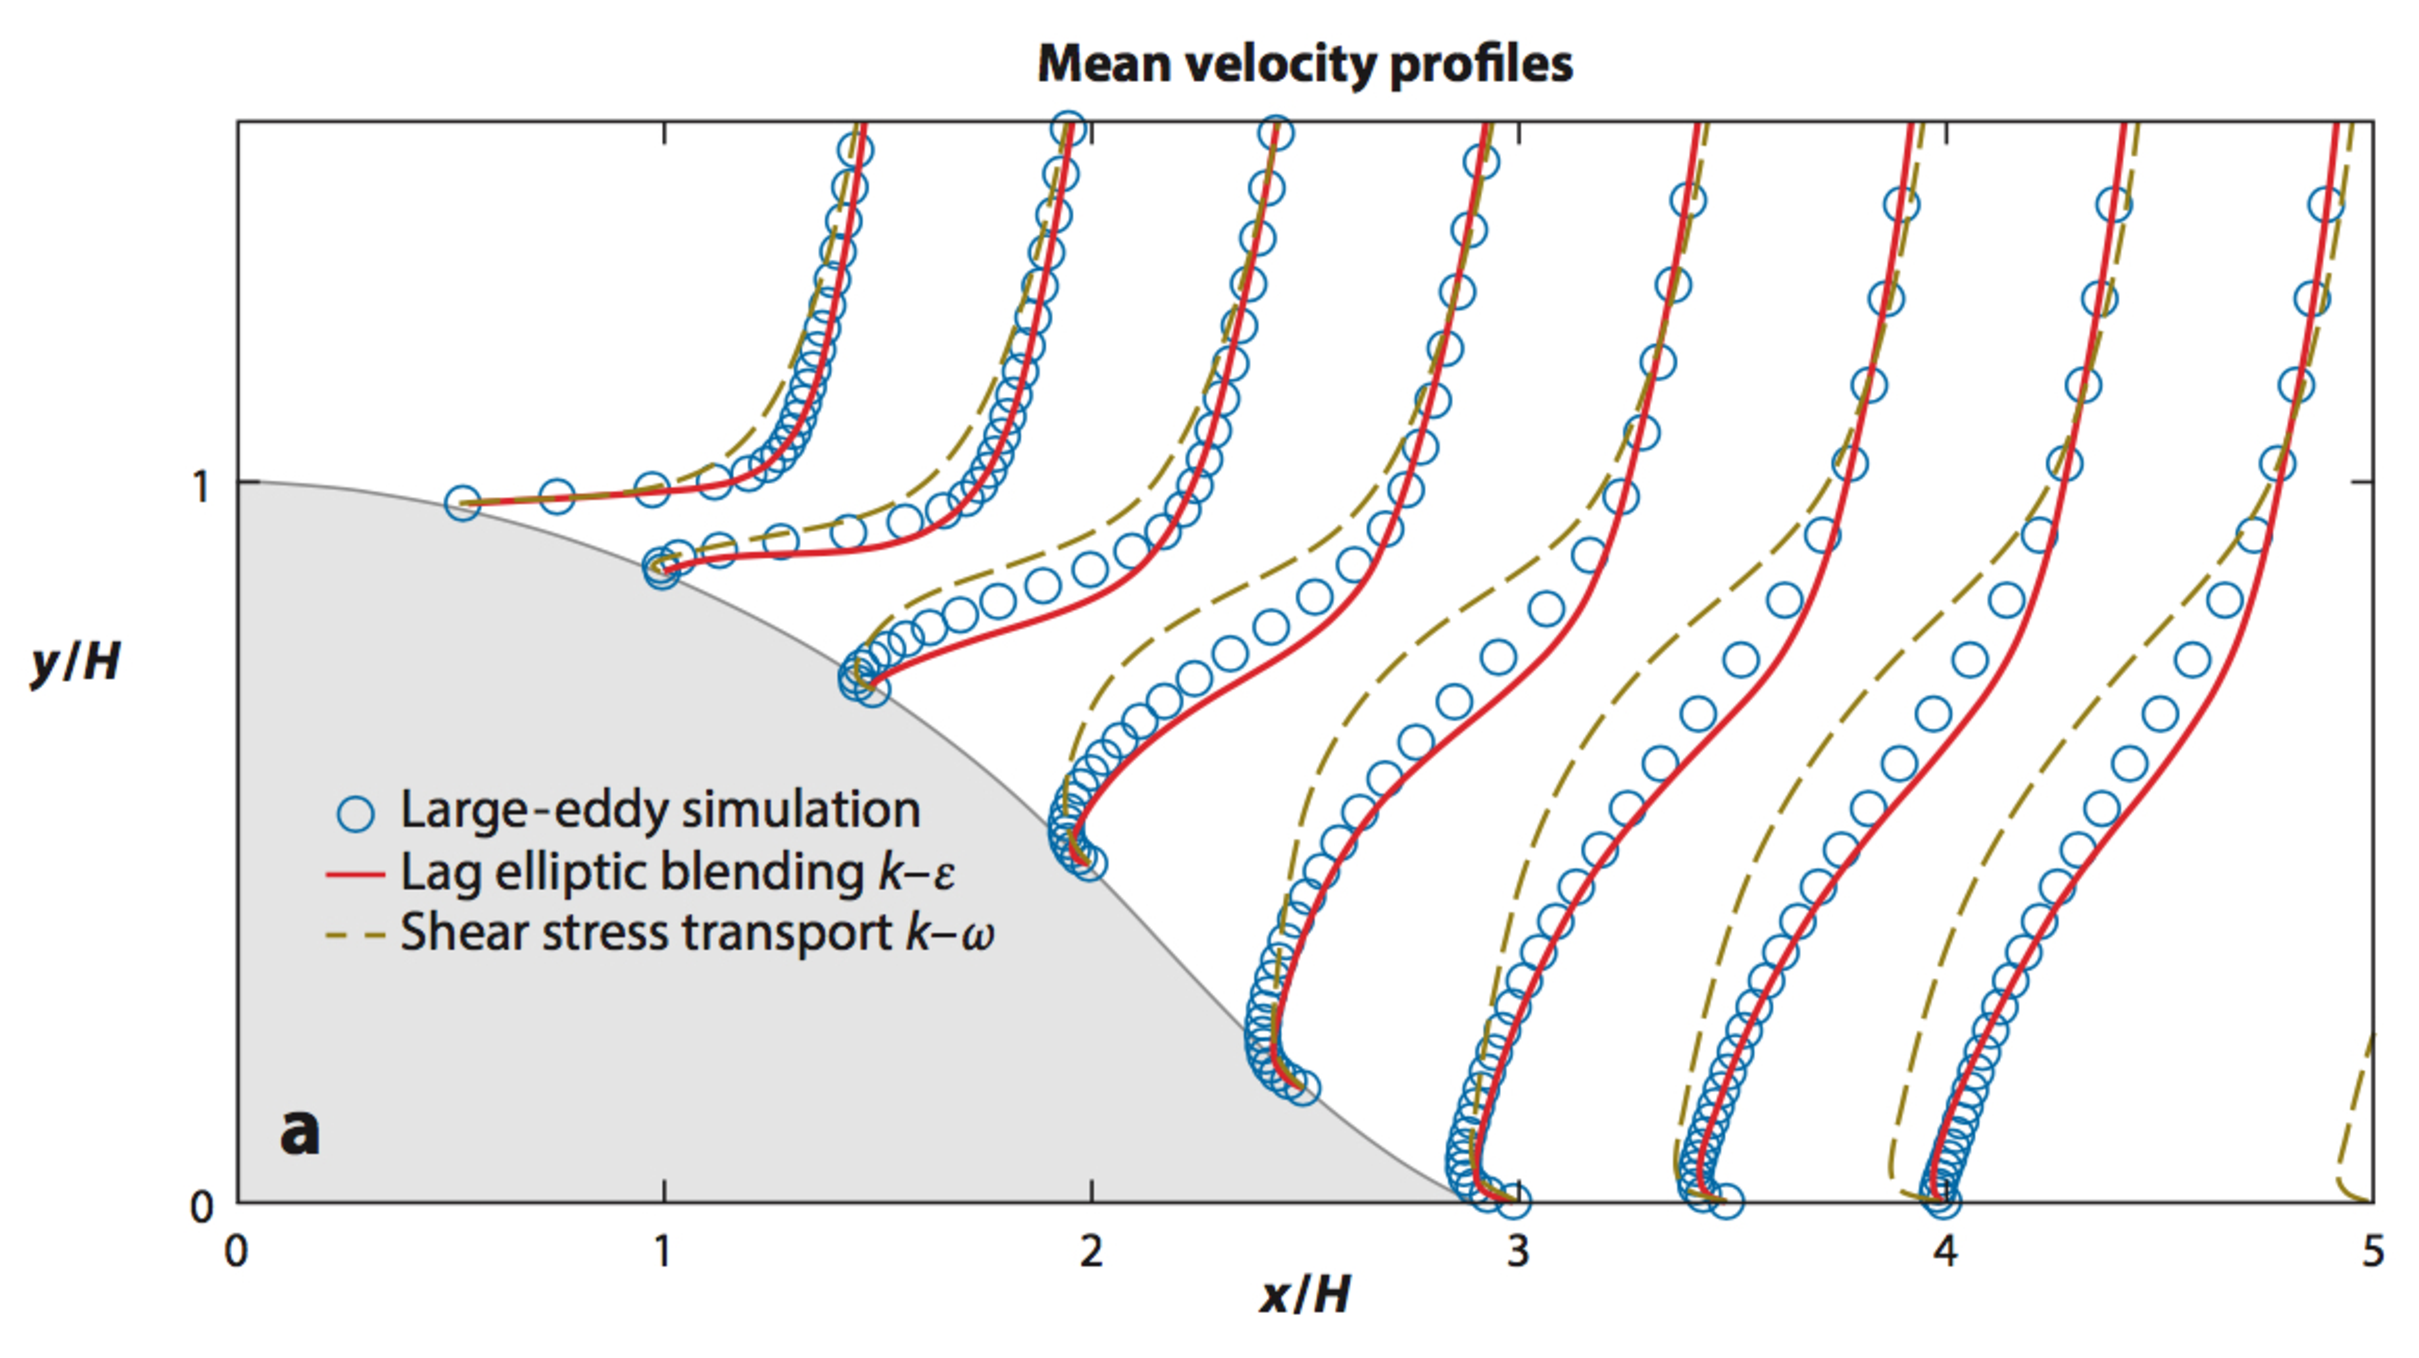
\includegraphics[width=0.5\textwidth]{Images/logan/durbin2018some_BackstepLESvsRANS.pdf}
\caption{curve backstep velocity profile les vs rans \cite{durbin2018some}}
\label{fig:lesvsransbackstep}
\end{center}
\end{figure}
%%\vspace{-2em}







%%% GOLF BALL DNS
%%\vspace{-2em}
% \begin{figure}[htb]
\begin{figure}[H]
\begin{center}
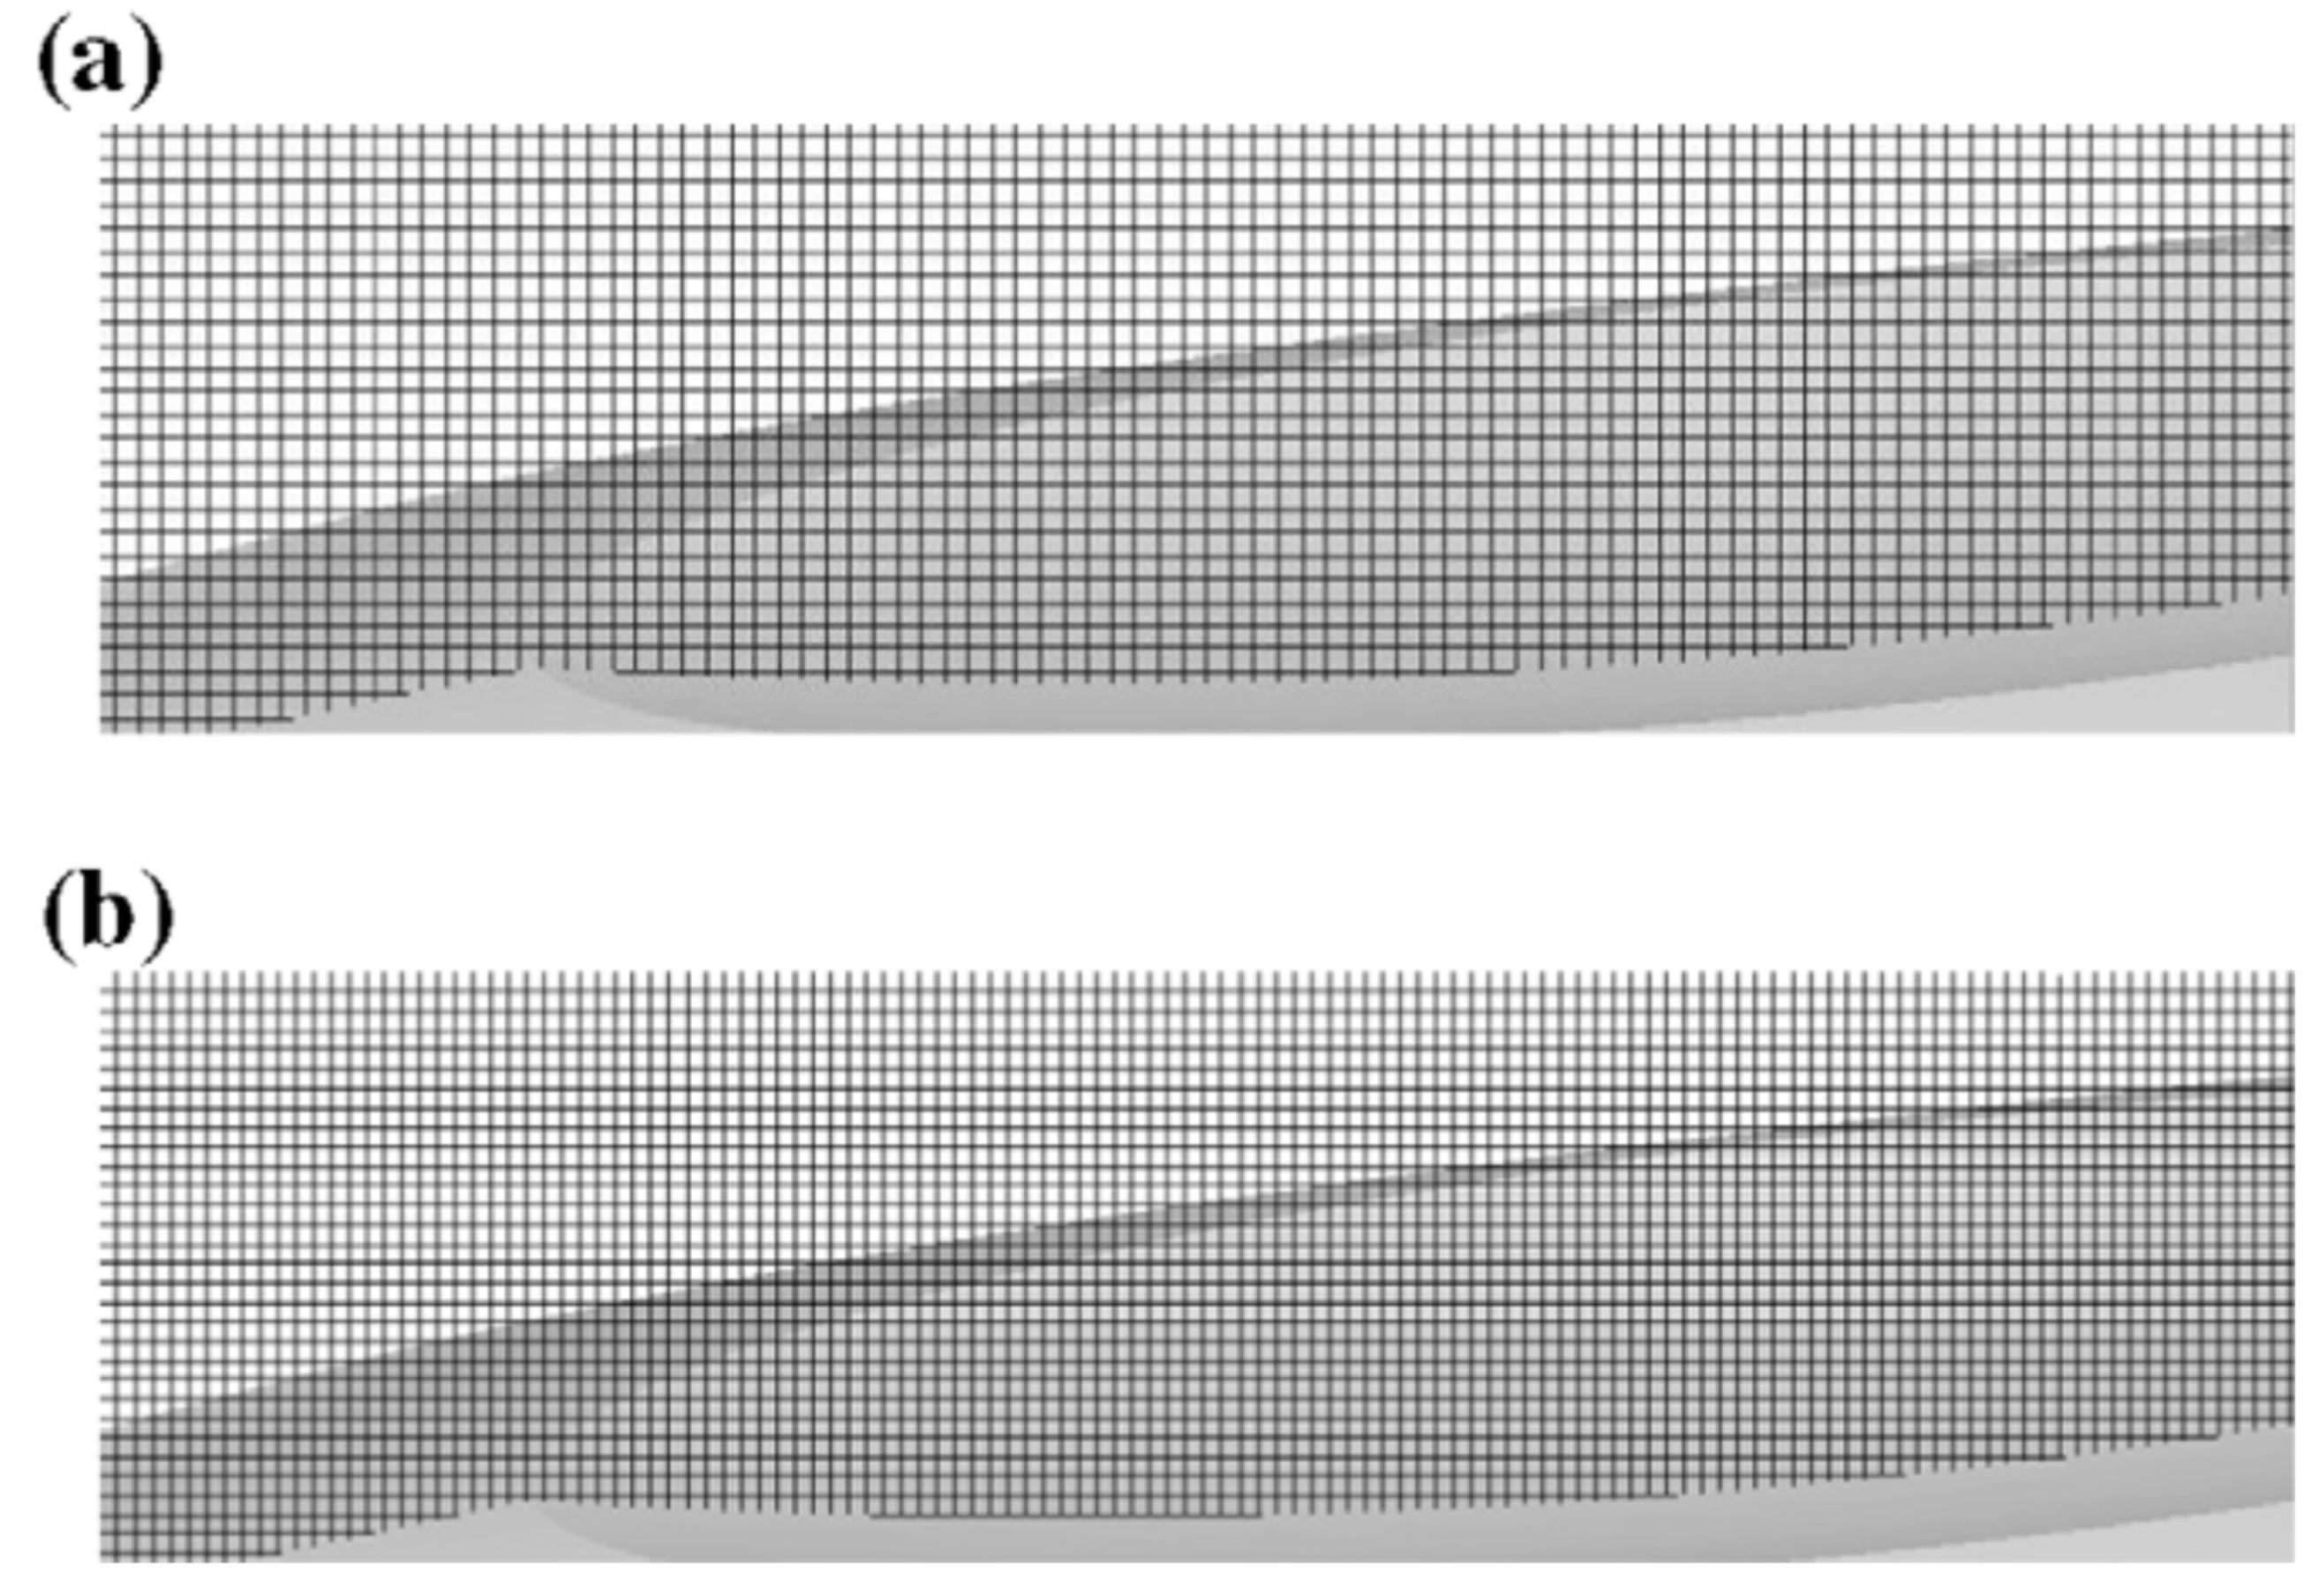
\includegraphics[width=0.45\textwidth]{Images/logan/smith2010numerical_golfballgrid.pdf}
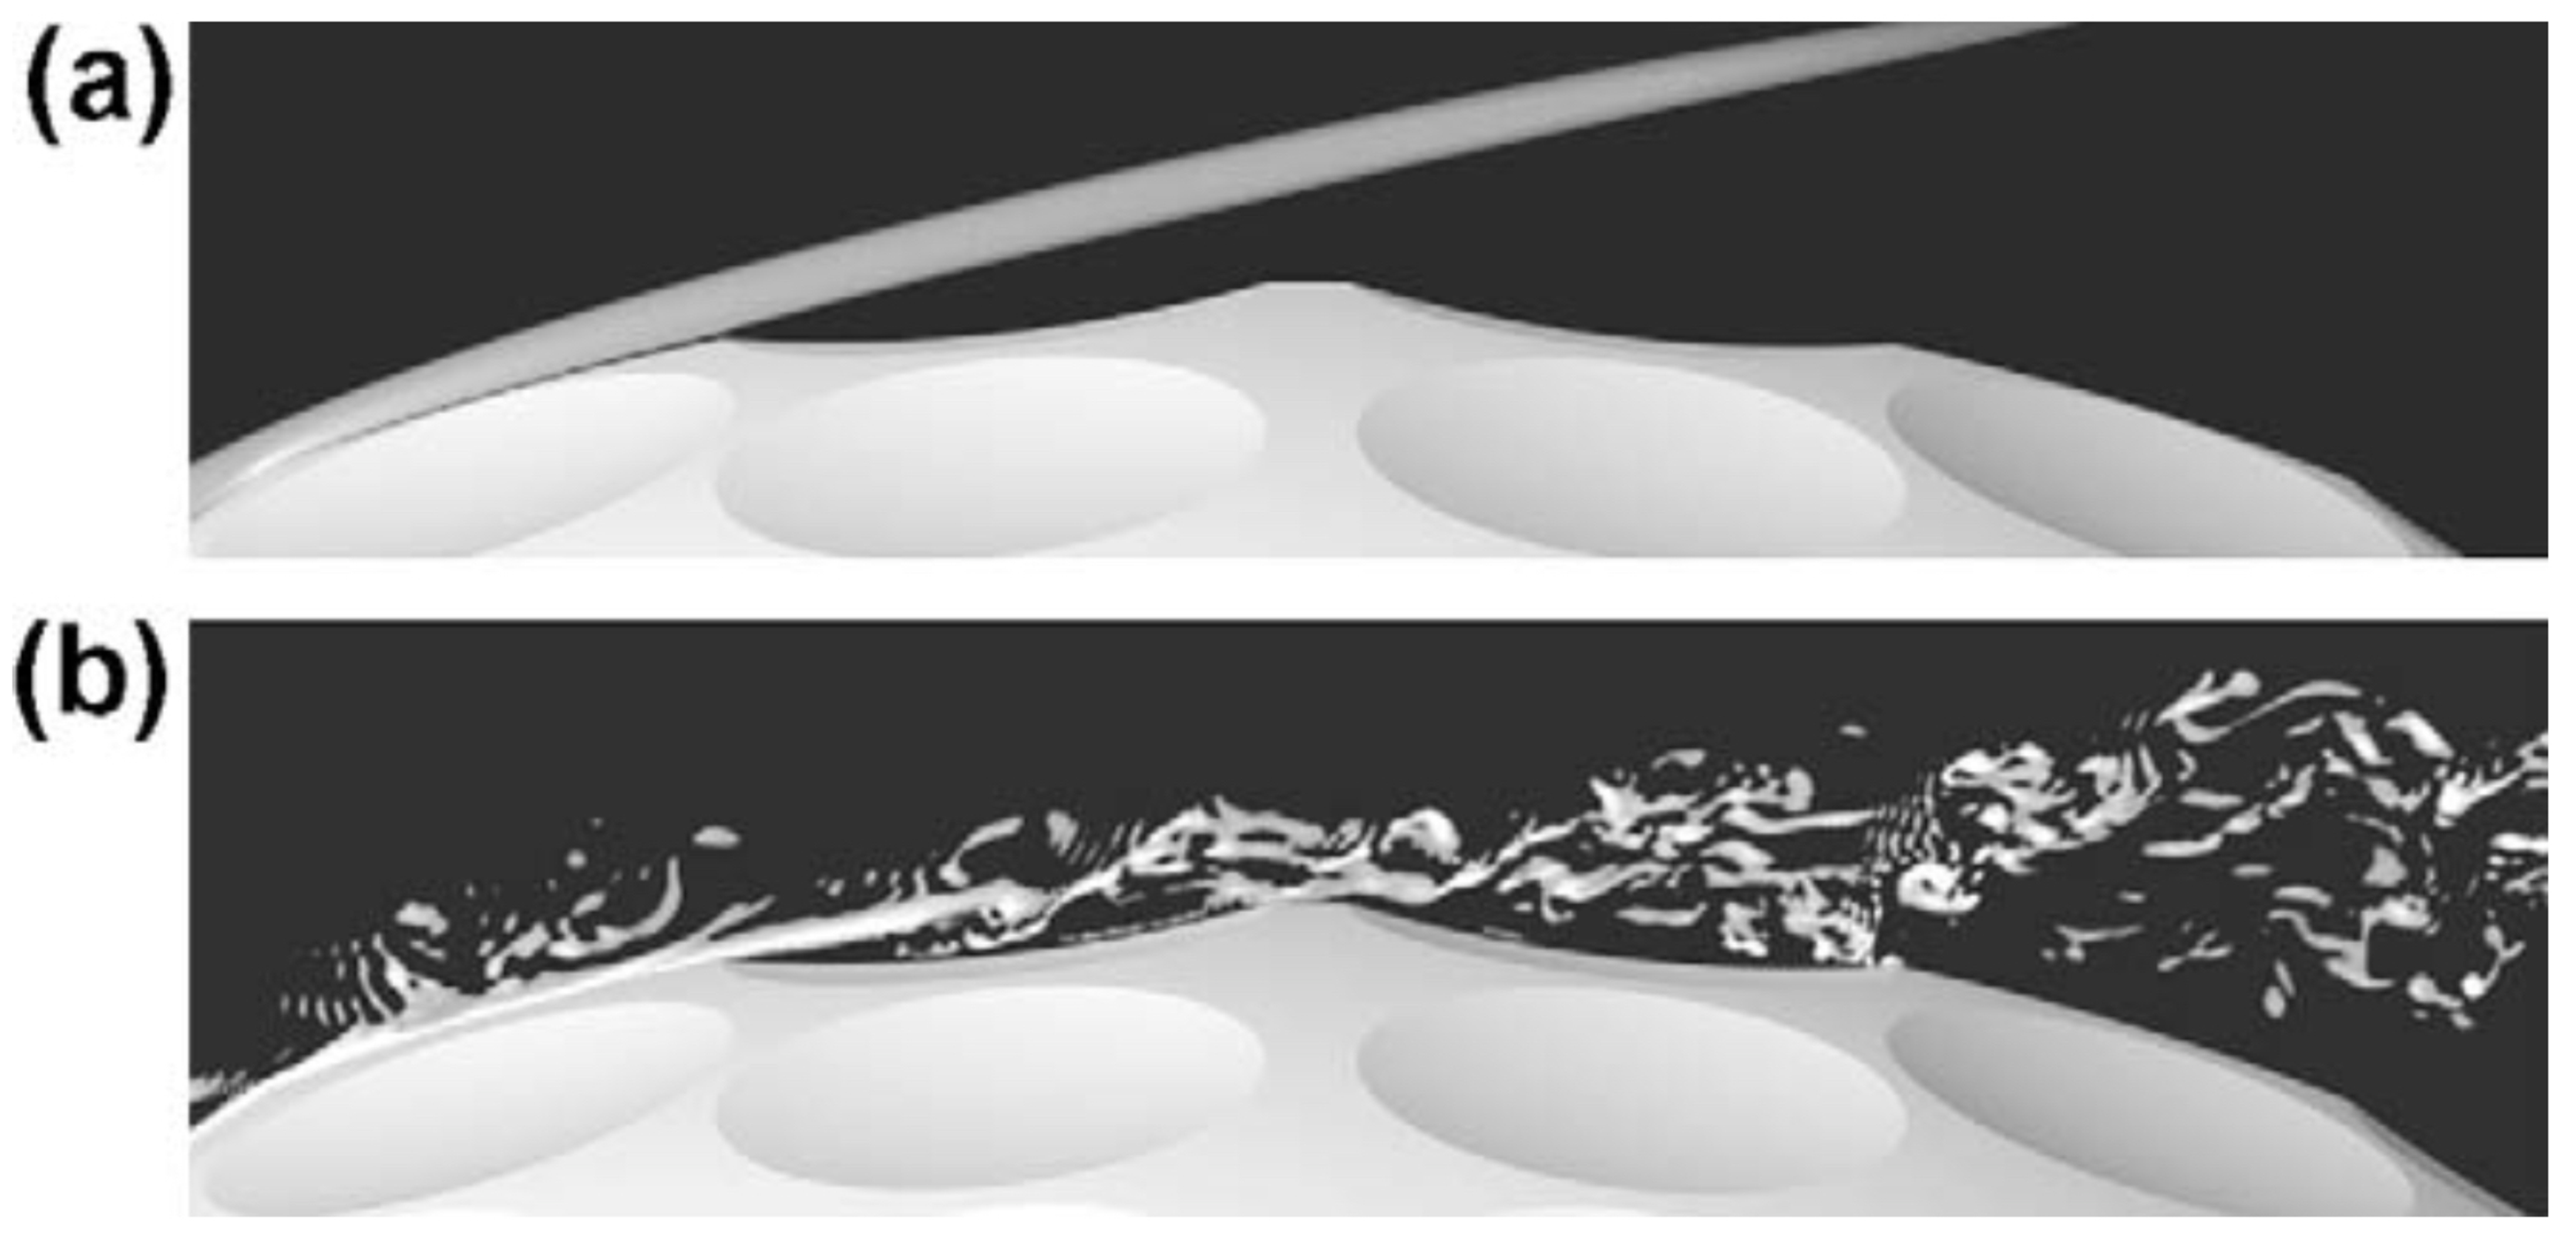
\includegraphics[width=0.45\textwidth]{Images/logan/smith2010numerical_golfballvorticity.pdf}
\caption{ DNS non-rotating golf ball with dimples grid (left) vorticity (right) \cite{smith2010numerical} }
\label{fig:dnsgolfball}
\end{center}
\end{figure}
%%\vspace{-2em}


Example grid resolution in a dimple near 84° (measured from the stagnation point at the front of the golf ball). (a) Re = 2.5   104; (b) Re = 1.1   105.

Contours of azimuthal vorticity. (a) Re = 2.5   104; (b) Re = 1.1   105

NOTE: Recall sphere example from Spalart review and say that this is the analogous DNS experiment to his DES


%%% RECTANCULAR CYLINDER DNS
%%\vspace{-2em}
% \begin{figure}[htb]
\begin{figure}[H]
\begin{center}
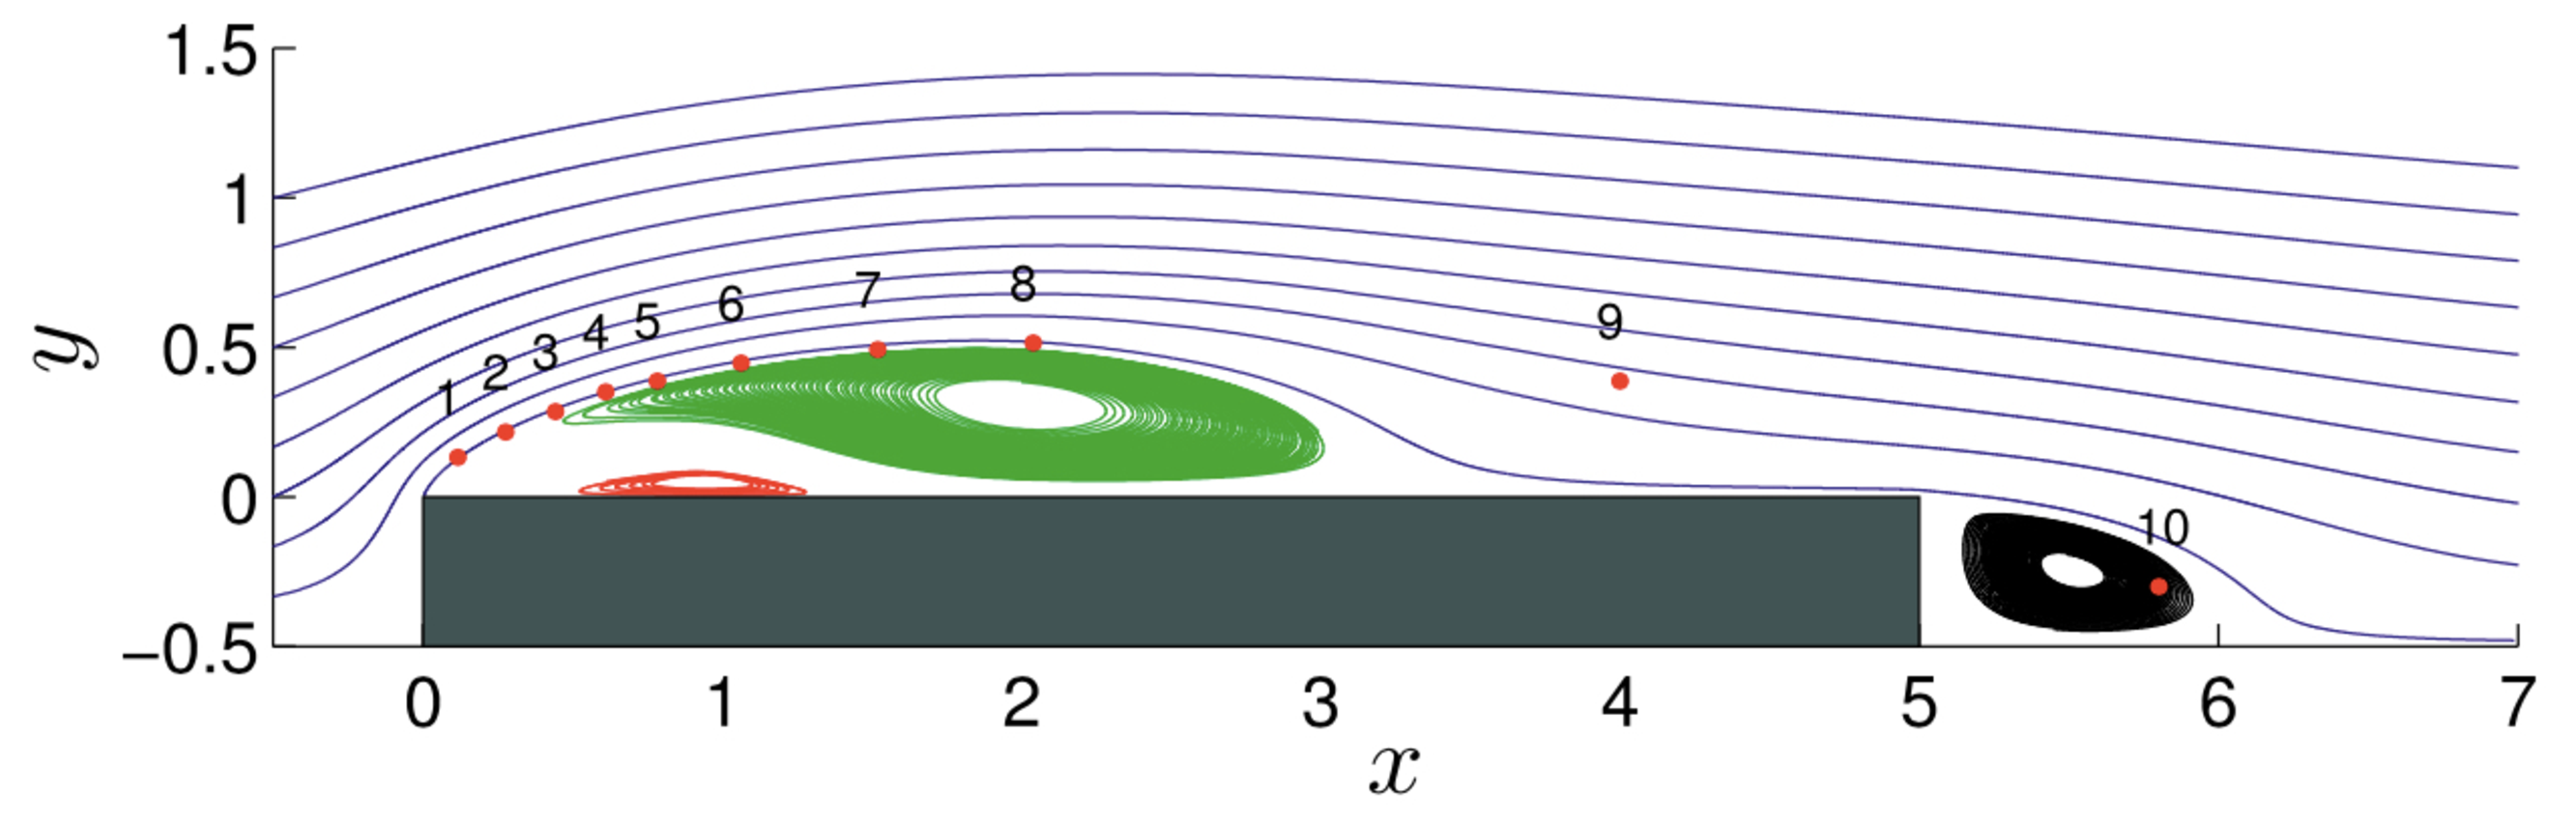
\includegraphics[width=0.45\textwidth]{Images/logan/cimarelli2018direct_vortices.pdf}
\caption{ DNS square cylinder vortex locations Re=3000 \cite{cimarelli2018direct} }
\label{fig:dnsRectCylVortices}
\end{center}
\end{figure}
%%\vspace{-2em}


Fig. 4. Streamlines of the mean velocity field (U,V) (x,y)  The green lines show the primary vortex, the red lines mark the secondary vortex and the black lines denote the wake vortex. The red dots denote the locations of the probes used for the computation of time spectra in section x5. (For interpretation of the references to color in this figure legend, the reader is referred to the Web version of this article.)

%%\vspace{-2em}
% \begin{figure}[htb]
\begin{figure}[H]
\begin{center}
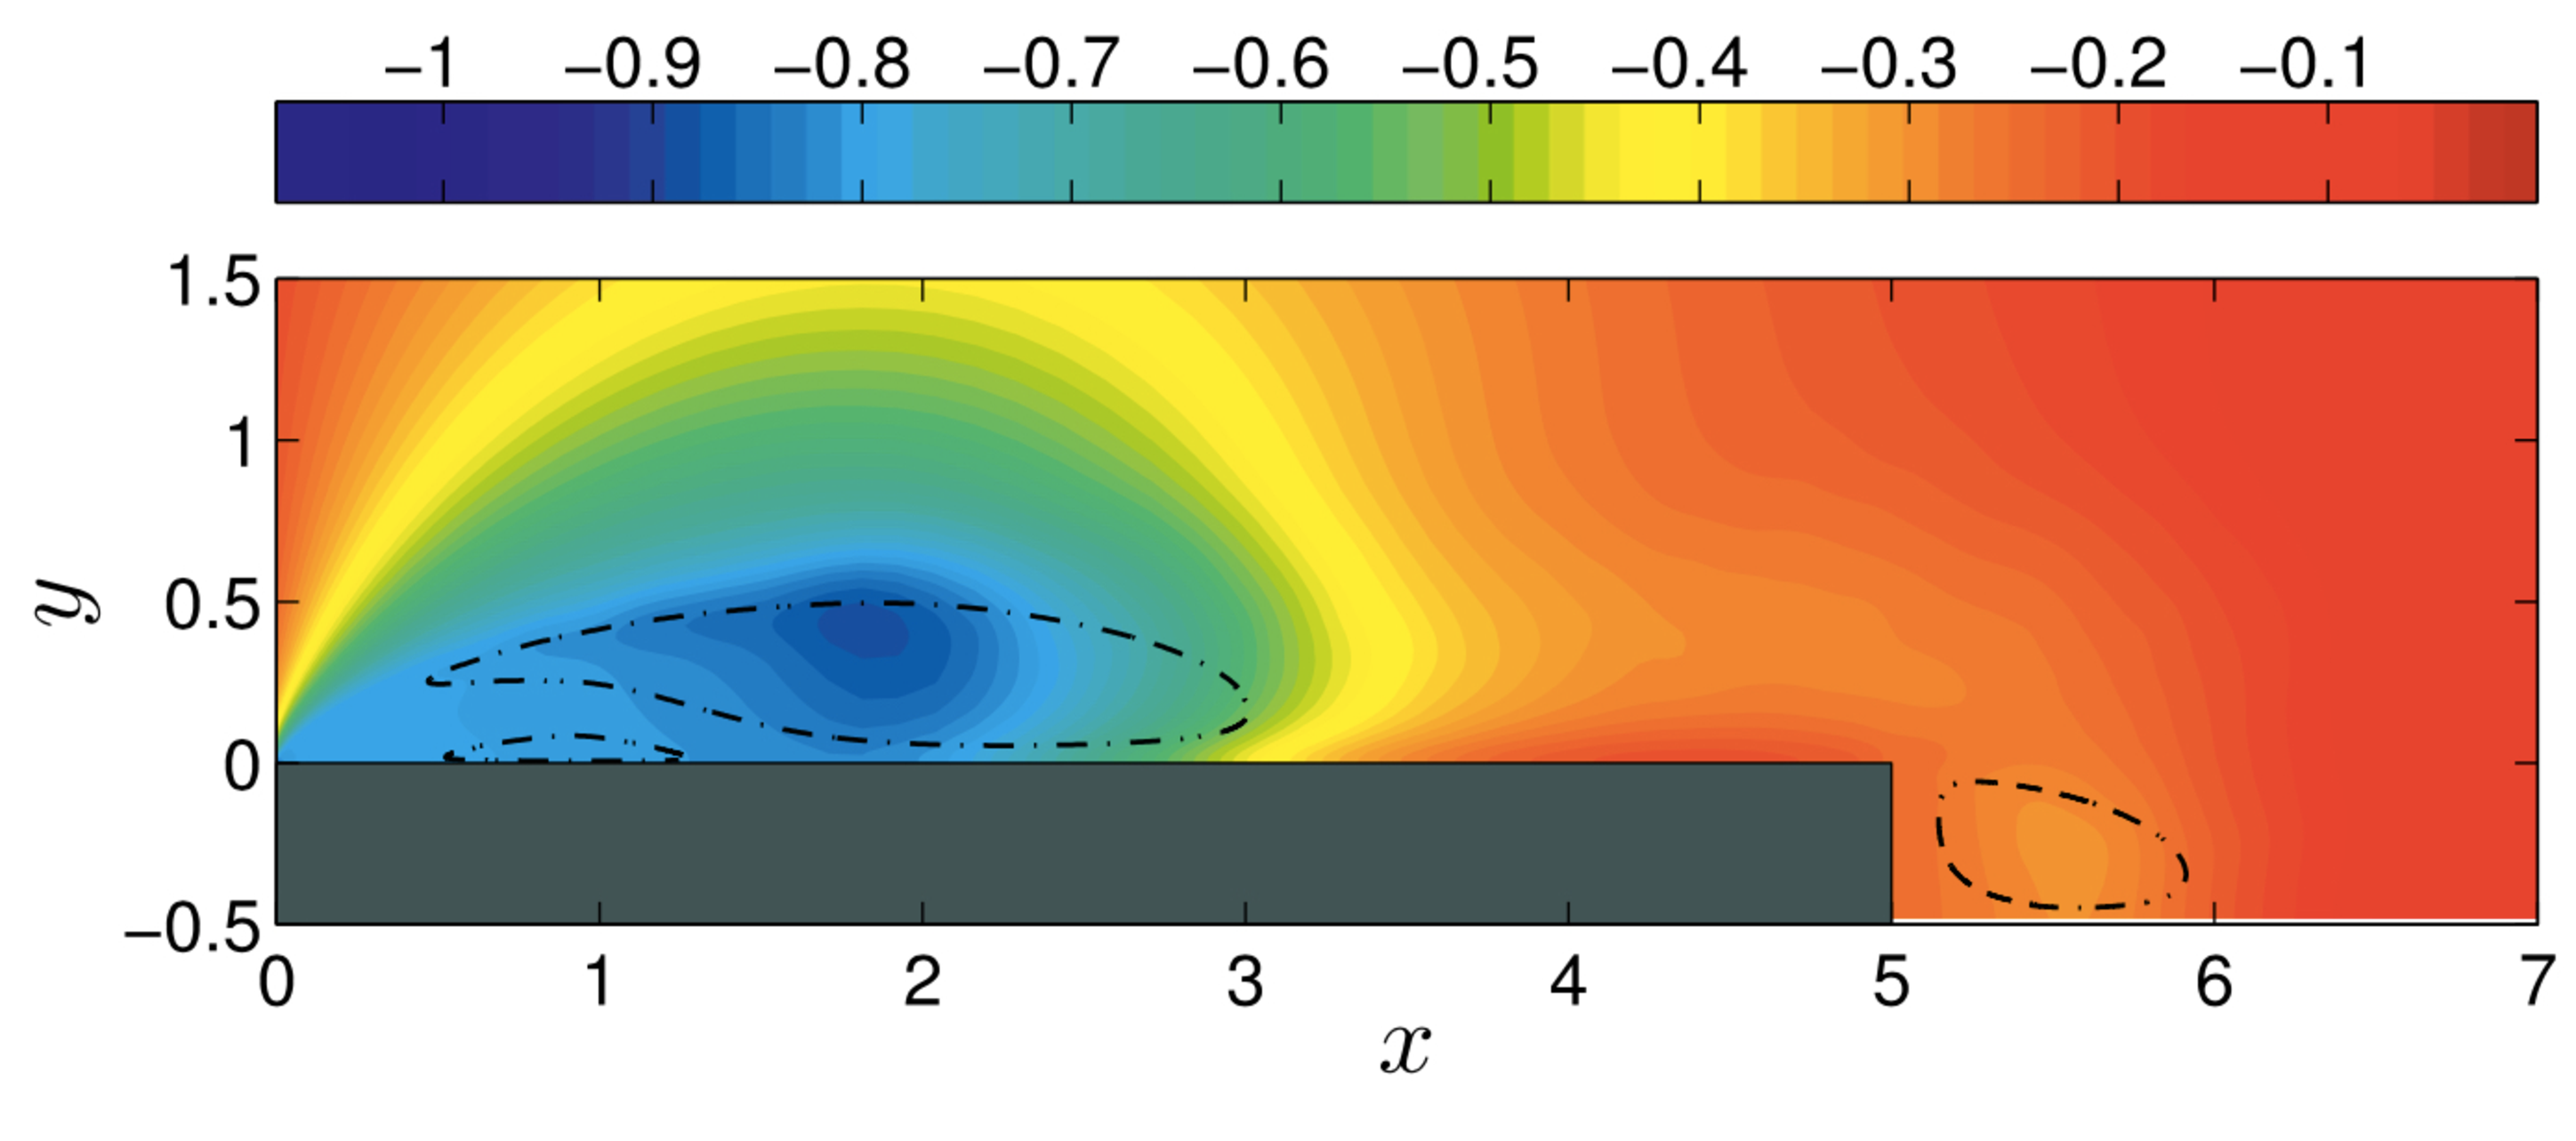
\includegraphics[width=0.45\textwidth]{Images/logan/cimarelli2018direct_pressure.pdf}
\caption{ DNS square cylinder mean pressure distribution Re=3000 \cite{cimarelli2018direct} }
\label{fig:dnsRectCylPressure}
\end{center}
\end{figure}
%%\vspace{-2em}

Fig. 5. Isocontours of the mean pressure field P(x,y). The dashed lines report the location of the primary vortex, secondary vortex and wake vortex.


%%\vspace{-2em}
% \begin{figure}[htb]
\begin{figure}[H]
\begin{center}
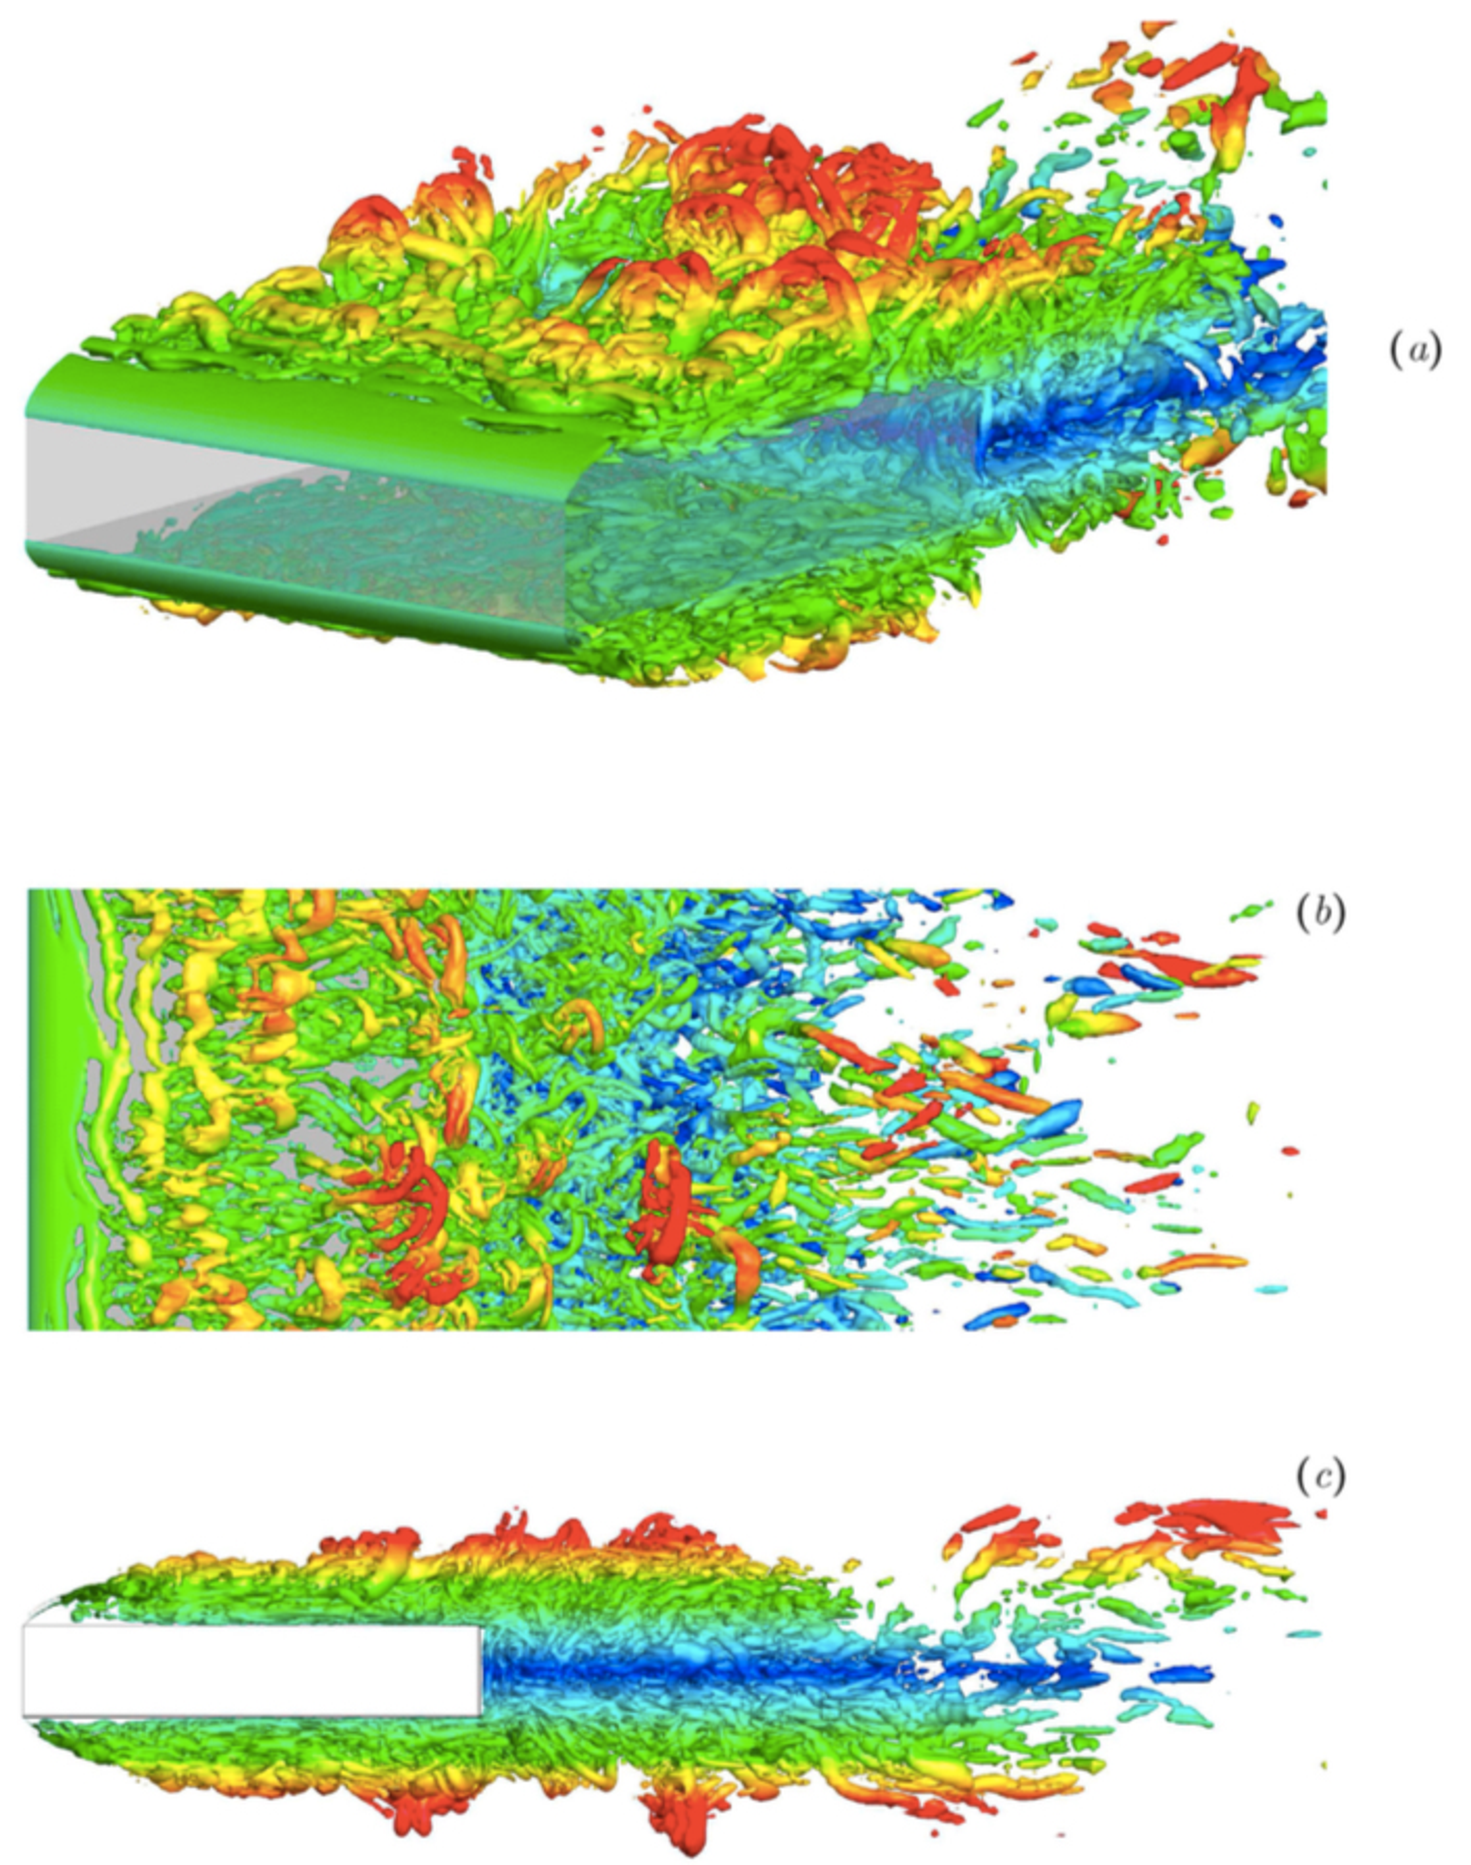
\includegraphics[width=0.5\textwidth]{Images/logan/cimarelli2018direct_vorticity.pdf}
\caption{ DNS square cylinder vorticity contours Re=3000 \cite{cimarelli2018direct} }
\label{fig:dnsRectCylPressure}
\end{center}
\end{figure}
%%\vspace{-2em}

Fig. 10. Instantaneous isosurfaces of $\lambda_2=-2$ colored with $y$. Perspective, top and lateral views in (a), (b) and (c) plots, respectively.































%%%%%%%%%%%%%%%%%%%%%%%%%%%%%%%%%%%%%%%%%%%%%%%%%%%%%%%%%%%%%%%%%%%%%%%%
\section{Current State of Bluff-Body Turbulence Analysis} \label{sec:currentstate}
%%%%%%%%%%%%%%%%%%%%%%%%%%%%%%%%%%%%%%%%%%%%%%%%%%%%%%%%%%%%%%%%%%%%%%%%

\begin{itemize}
    \item Current State of Knowledge
    \item Remaining Challenges
\end{itemize}


%%%%%%%%%%%%%%%%%%%%%%%%%%%%%%%%%%%%%%%%%%%%%%%%%%%%%%%%%%%%%%%%%%%%%%%%
\subsection{Experimental Methods} \label{subsec:currentstateexperimental}

\textcolor{red}{\emph{FZ}}


%%%%%%%%%%%%%%%%%%%%%%%%%%%%%%%%%%%%%%%%%%%%%%%%%%%%%%%%%%%%%%%%%%%%%%%%
\subsection{Computational Methods} \label{subsec:currentstatecomputational}



\textcolor{red}{\emph{LH}}














%%%%%%%%%%%%%%%%%%%%%%%%%%%%%%%%%%%%%%%%%%%%%%%%%%%%%%%%%%%%%%%%%%%%%%%%
\section{Conclusions}
%%%%%%%%%%%%%%%%%%%%%%%%%%%%%%%%%%%%%%%%%%%%%%%%%%%%%%%%%%%%%%%%%%%%%%%%

\textcolor{red}{\emph{LH\&FZ}}



%%%%%%%%%%%%%%%%%%%%%%%%%%%%%%%%%%%%%%%%%%%%%%%%%%%%%%%%%%%%%%%%%%%%%%%%
\section*{Acknowledgments} %%%%%%%%%%%%%%%%%%%%%%%%%%%%%%%%%%%%%%%%%%%%%
%%%%%%%%%%%%%%%%%%%%%%%%%%%%%%%%%%%%%%%%%%%%%%%%%%%%%%%%%%%%%%%%%%%%%%%%

\textcolor{red}{\emph{LH\&FZ}}

%%%%%%%%%%%%%%%%%%%%%%%%%%%%%%%%%%%%%%%%%%%%%%%%%%%%%%%%%%%%%%%%%%%%%%%%
%%% BIBLIOGRAPHY %%%%%%%%%%%%%%%%%%%%%%%%%%%%%%%%%%%%%%%%%%%%%%%%%%%%%%%
%%%%%%%%%%%%%%%%%%%%%%%%%%%%%%%%%%%%%%%%%%%%%%%%%%%%%%%%%%%%%%%%%%%%%%%%

%SAMPLE CITATIONS TO SEE CITATION FORMATTING
\textcolor{red}{Example citations}

\cite{nakamura1993bluffbody}

%bibliography from .bib file, filename goes in {}
%NOTE: References must be cited with "\cite" command to appear in bibliography
%Types of Refs: article, book, conference=inproceedings, manual, mastersthesis, phdthesis, techreport, unpublished, misc (see "new-aiaa.bst")
%when you first initialize .bib file, might need to have plain text in front of \cite command to get sublime text to recognize bibliography file
\bibliography{BluffBodyTurb}

\end{document}
